%% 
%% This is a sample doctoral dissertation.  It shows the appropriate
%% structure for your dissertation.  It should handle most of the
%% strange requirements imposed by the Grad school; like the different
%% handling of titles of one/many appendices.  It will automatically
%% handle the linespacing changes.  The body default is double-spaced
%% (except when you use the singlespace or condensed options).  The
%% default for quotations is single-space, and the default for tabular
%% environments is also single-space.  
%%
%% This class adds the following commands and environments to the
%% report class, upon which it is based:
%% Commands
%% ------------
%% \degree{name}{abbrv} -- Sets the name and abbreviation for the degree.
%%                         These default to ``Doctor of Philosopy''
%%                         and ``Ph.D.'', respectively.
%% \copyrightyear{year} -- for the copyright page.
%% \bachelors{degree}{institution} -- for the abstract
%% \masters{degree}{institution}   --  "
%%     if you have other degrees you may use
%% \secondbachelors{degree}{institution}
%% \thirdbachelors{degree}{institution}
%% \secondmasters{degree}{institution}
%% \thirdmasters{degree}{institution}
%% \priordoctorate{degree}{institution}
%%
%% \committeechair{name}           -- for the signature page
%% or, if you have two co-chairs:
%% \cochairs{first name}{second name}
%%
%% \firstreader{name}              --  "
%% \secondreader{name}             --  "
%% \thirdreader{name}              -- (optional)
%% \fourthreader{name}             --  "
%% \fifthreader{name}              --  "
%% \sixthreader{name}              --  "
%% \departmentchair{name}          -- for the signature page
%% \departmentname{name}           --  "
%%
%% \copyrightpage                  -- produces the copyright page
%% \signaturepage                  -- produces the signature page
%%
%% \frontmatter                    -- these are required in their various
%% \mainmatter                     -- appropriate locations
%% \backmatter                     --
%%
%% \unnumberedchapter[toc]{name}   -- like \chapter, except that it
%%                                    produces an unnumbered chapter;
%%                                    alternatively, like \chapter*,
%%                                    except that it lists the chapter
%%                                    in the table of contents.
%%
%% New environments:
%%   dedication  -- for the dedication
%%   abstract    -- for the abstract
%%
%% The thesis documentclass is built on top of the report document class.
%% It accepts all of the options that the report class accepts, plus the
%% following:
%%     doublespace -- the default, indicates double spacing as per U.Mass.
%%                    requirements.  You will need this when you do your
%%                    final copy.
%%     singlespace -- for earlier work, not acceptable to the Grad school
%%     condensed   -- for earlier work, not acceptable to the Grad school,
%%                    creates condensed versions of the frontmatter. 
%%                    Condensed implies singlespace.
%%     dissertation - the default, indicates that this document is a
%%                    dissertation.
%%     proposal    -- indicates that this document is a dissertation proposal,
%%                    rather than a dissertation.  This will only change the
%%                    wording on the title and signature pages.
%%     thesis      -- indicates that this document is a Master's thesis 
%%                    rather than a doctoral dissertation.  This also changes
%%                    the default for \degree to Master of Science, M.S.
%%     allowlisthypenation -- (the default), allows hyphenation of words in
%%                    the table of contents, the list of figures, and the list
%%                    of tables.  I believe that this is acceptable to the 
%%                    Graduate School.
%%     nolisthyphenation -- disallows hyphenation of words in the table of
%%                    contents and the list of figures and tables.  Use this 
%%                    option if the Grad School doesn't like your hyphenation.
%%     nicerdraft  -- relaxes some of the Grad School's rules for working with
%%                    drafts -- has no effect when doublespace is in effect
%%     nonicerdraft -- the default, leaves things in draft as they will be in
%%                     the final version
%% umassthesis changes the default font size to 12pt, but you may specify 10pt or
%%   11pt in the options.
\documentclass{umassthesis}          % for Ph.D. dissertation or proposal
% \documentclass[thesis]{umassthesis}  % for Master's thesis

%%
%% If you have enough figures or tables that you run out of space for their
%% numbers in the List of Tables or List of figures, you can use the following
%% command to adjust the space left for numbers.  The default is shown:
%%
%% \setlength{\tablenumberwidth}{2.3em}

%% Use the hyperref package if you're producing a version for online
%% distribution and you want hyperlinks.  Note that the Grad School doesn't want
%% their PDF viewers to colorize or otherwise highlight the links; use the
%% hidelinks option to hyperref to avoid decorating links.
\usepackage[hidelinks]{hyperref}
\usepackage{thesis-defs}
\usepackage{graphicx}
\usepackage{amsmath}
\usepackage{subfig}
%% One way of formatting the epigraph/frontispiece is to use this package.
% \usepackage{epigraph}

\begin{document}

%%
%% You must fill in all of these appropriately
\title{Measurement of the Higgs boson production cross section in association with a vector boson and decaying into $WW^{*}$ with the ATLAS detector at $\sqrt{s}$ = 13.6 TeV}
\author{Matthew L. Harris}
\date{October 2025} % The date you'll actually graduate -- must be
                     % February, May, or September
\copyrightyear{2025}
\bachelors{B.Sc.}{University of Massachusetts, Amherst}
\masters{M.Sc.}{University of Massachusetts, Amherst}
% \secondmasters{M.Ed.}{Antioch College}
% \priordoctorate{M.D.}{University of Never-never-land}
\committeechair{Stephane Willocq}
% \cochairs{B. B. Bahh}{I. M. A. Wolf}
\firstreader{Carlo Dallapicolla}
\secondreader{Lorenzo Sorbo}
\thirdreader{Robert Kusner}
% \fourthreader{Robert Kusner}   % Optional
%\fifthreader{}            % Optional
%\sixthreader{}            % Optional
\departmentchair[Department Chair]{Name of Dept Head} % Default uses "Department Chair" as the title. To
% use an alternate title, such as "Chair", use \departmentchair[Chair]{Pete Shearer}
% CICS uses "Chair of the Faculty" as of 2019.
\departmentname{Physics}
% \departmentname{Robert and Donna Manning College of \\Information and Computer Sciences}


%% If your degree is something other than a Ph.D. (for a dissertation), or
%% an M.S. (for a thesis), you will need to uncomment the appropriate
%% following line:
%%
%% \degree{Doctor of Education}{Ed.D.}
\degree{Doctor of Philosophy}{Ph.D.}
%%
%% \degree{Master of Arts}{M.A.}
%% \degree{Master of Arts in Teaching}{M.A.T.}
%% \degree{Master of Business Administration}{M.B.A.}
%% \degree{Master of Education}{M.Ed.}
%% \degree{Master of Fine Arts}{M.F.A.}
%% \degree{Master of Landscape Architecture}{M.L.A.}
%% \degree{Master of Music}{M.M.}
%% \degree{Master of Public Administration}{M.P.A.}
% \degree{Master of Public Health}{M.P.H.}
%% \degree{Master of Regional Planning}{M.R.P.}
%% \degree{Master of Science}{M.S.}
%% \degree{Master of Science in Accounting}{M.S. Acctg.}
%% \degree{Master of Science in Chemical Engineering}{M.S. Ch.E.}
%% \degree{Master of Science in Civil Engineering}{M.S.C.E.}
%% \degree{Master of Science in Electrical and Computer Engineering}{M.S.E.C.E.}
%% \degree{Master of Science in Engineering Management}{M.S. Eng. Mgt.}
%% \degree{Master of Science in Environmental Engineering}{M.S. Env. E.}
%% \degree{Master of Science in Industrial Engineering and Operations Research}{M.S.I.E.O.R.}
%% \degree{Master of Science in Manufacturing Engineering}{M.S. Mfg. Eng.}
%% \degree{Master of Science in Mechanical Engineering}{M.S.M.E.}
%%
%% \degree{Professional Master of Business Administration}{P.M.B.A.}


%%
%% These lines produce the title, copyright, and signature pages.
%% They are Mandatory; except that you could leave out the copyright page
%% if you were preparing an M.S. thesis instead of a PhD dissertation.
\frontmatter
\maketitle
\copyrightpage{}     %% not required for an M.S. thesis
\signaturepage{}

%%
%% Dedication is optional -- but this is how you create it
% \begin{dedication}              % Dedication page
%   \begin{center}
%     \emph{To those little lost sheep.}
%   \end{center}
% \end{dedication}

%%
%% Epigraph (aka frontispiece) is also optional, but this is one way you
%% can create it
%\begin{frontispiece}
%  %% Format to your liking -- see documentation of epigraph package
%  \setlength{\epigraphrule}{0pt}
%
%  \begin{epigraphs}
%    \qitem{%
%      \itshape
%      Mary had a little lamb,\\
%      Her fleece was white as snow.\\
%      \vspace{\baselineskip}
%      And everywhere that Mary went\\
%      The lamb was sure to go.
%      \vspace{\baselineskip}}
%    {Sarah Josepha Hale}
%
%    \vspace{2\baselineskip}
%    \qitem{%
%      \itshape
%      Baa, baa, black sheep,\\
%      Have you any wool?\\
%      Yes, sir, yes, sir,\\
%      Three bags full;\\
%      One for the master,\\
%      And one for the dame,\\
%      And one for the little boy\\
%      Who lives down the lane.
%      \vspace{\baselineskip}}
%    {English Nursery Rhyme}
%
%  \end{epigraphs}
%\end{frontispiece}

%%
%% Acknowledgements are optional...yeah, right.
\chapter{Acknowledgments}             % Acknowledgements page
  Fill in later

%%
%% Abstract is MANDATORY. -- Except for MS theses
\begin{abstract}                % Abstract
    Abstract will be filled in later
\end{abstract}

%%
%% Preface goes here...would be just like Acknowledgements -- optional
%% \chapter{Preface} 
%% ...


%%
%% Table of contents is mandatory, lists of tables and figures are 
%% mandatory if you have any tables or figures; must be in this order.
\tableofcontents                % Table of contents
\listoftables                   % List of Tables
\listoffigures                  % List of Figures

%%
%% We don't handle List of Abbreviations
%% We don't handle Glossary

%%%%%%%%%%%%%%%%%%%%%%%%%%%%%%%%%%%%%%%%%%%%%%%%%%%%%%%%%%%%%%%%%%%%%%%%%
%% Time for the body of the dissertation
\mainmatter{}   %% <-- This line is mandatory

%%
%% If you want an introduction, which is not a numbered chapter, insert
%% the following two lines.  This is OPTIONAL:
\unnumberedchapter{Introduction}\label{ch:introduction}
The Standard Model (SM) of elementary particle physics is, to date, the best description that physicists have of fundamental interactions. This theory, which was developed throughout the
20th century, has been supported by numerous experimental observations and predicts key measurements with extreme precision. 

In June of 2012, the last missing piece of the standard model was finally observed at the Large Hadron Collider (LHC), the Higgs boson. In a joint announcement, both the ATLAS~\cite{ATLAS_Higgs_discovery} and CMS~\cite{CMS_Higgs_discovery} collaborations announced the discovery of a particle consistent with the Higgs boson at the approximate mass of
125 GeV. Since the discovery, many precision measurements of the Higgs boson have occurred between both collaborations, further confirming properties of the Higgs boson that are predicted by the Standard Model. Although the Standard Model has held up very well with all of its predictions, it has also been well established that the Standard Model is not a complete theory, with many key phenomenon still unexplained. 
For example, the Standard Model does not address dark matter or dark energy which together, make up a large part of the universe. Furthermore, gravity is not explained, offers no explanation for the matter-antimatter asymmetry, and suffers from the so-called `naturalness problem', which arises due to fine-tuning of the Higgs boson's mass to prevent large quantum corrections, a situation considered unnatural and indicative of missing physics.

Many extensions of the Standard Model, referred to as beyond the Standard Model (BSM), have been proposed to address its limitations mentioned previously, including the infamous, and most well known, supersymmetry~\cite{MARTIN_1998}, which introduces a new symmetry between bosons and fermions and offers solutions to some of the previously mentioned issues. However, after extensive searching, there has been no experimental evidence that supersymmetry exists.
In addition to direct BSM searches, model-independent approaches have also been developed that look for deviations from the Standard Model in precision measurements. One of these approaches is known as the Simplified Template Cross Sections~\cite{STXS_1_1} (STXS) framework, which has been developed centrally at the LHC via the LHC Higgs Working Group. This framework defines a set of fiducial regions in phase space which aims to maximize sensitivity to BSM effects while also minimizing dependence on theoretical predictions.

One such way to interpret potential deviations in a systematic way is to use Standard Model Effective Field Theory (SMEFT). This essentially extends the Standard Model lagrangian via perturbations and allows for the addition of higher order operators which are suppressed by higher energy scales. The strength of these operators is governed by parameters known as `Wilson coefficients'. By measuring cross sections in the STXS framework, and comparing to SMEFT predictions, constraints can be placed on the Wilson coefficients which allows us to probe BSM physics even without a direct signal.
An additional use of the STXS framework is that it allows for combination measurements with various decay channels, and even across experiments. These combinations provide increased statistical power and allow for more stringent testing of the Standard Model.

In this thesis, the inclusive, and several STXS cross sections, of Higgs boson production in association with a vector boson with the Higgs boson decay to $WW^{*}$ using 2022 and 2023 Run 3 ATLAS data will be presented. Chapter~\ref{ch:theory} will provide an overview of the Standard Model, and also a derivation of the Standard Model lagrangian. Afterwards, we will move on to talking specifically about the Higgs boson and its specific production and decay modes. Chapter~\ref{ch:atlas} will provide an overview of the LHC and ATLAS detector. Chapter~\ref{ch:data_mc} will discuss the datasets used in this analysis as well as the Monte Carlo simulations used. Chapter~\ref{ch:reco} will discuss event reconstruction with an emphasis on upgrade muon software work. Chapter~\ref{ch:nn} will discuss neural networks and illuminate the mysterious black box. Chapter~\ref{ch:vh_analysis} will discuss the VH analysis, and the different Higgs boson decay modes that were analyzed in this analysis. Chapter~\ref{ch:vh_inclusive_results} will discuss the results for the inclusive Higgs boson cross section measurement, and Chapter~\ref{ch:vh_stxs_results} will discuss cross section results in STXS bins.
Finally, we will conclude with a summary of the results and a discussion of future work in Chapter~\ref{ch:conclusions}.


% , while also discussing muon track reconstruction software for the future High-Luminosity LHC (HL-LHC)

%%
%% Some sample text
% \chapter{Introduction}\label{ch:introduction}
% The Standard Model (SM) of elementary particle physics is, to date, the best description that physicists have of fundamental interactions. This theory, which was developed throughout the
20th century, has been supported by numerous experimental observations and predicts key measurements with extreme precision. 

In June of 2012, the last missing piece of the standard model was finally observed at the Large Hadron Collider (LHC), the Higgs boson. In a joint announcement, both the ATLAS~\cite{ATLAS_Higgs_discovery} and CMS~\cite{CMS_Higgs_discovery} collaborations announced the discovery of a particle consistent with the Higgs boson at the approximate mass of
125 GeV. Since the discovery, many precision measurements of the Higgs boson have occurred between both collaborations, further confirming properties of the Higgs boson that are predicted by the Standard Model. Although the Standard Model has held up very well with all of its predictions, it has also been well established that the Standard Model is not a complete theory, with many key phenomenon still unexplained. 
For example, the Standard Model does not address dark matter or dark energy which together, make up a large part of the universe. Furthermore, gravity is not explained, offers no explanation for the matter-antimatter asymmetry, and suffers from the so-called `naturalness problem', which arises due to fine-tuning of the Higgs boson's mass to prevent large quantum corrections, a situation considered unnatural and indicative of missing physics.

Many extensions of the Standard Model, referred to as beyond the Standard Model (BSM), have been proposed to address its limitations mentioned previously, including the infamous, and most well known, supersymmetry~\cite{MARTIN_1998}, which introduces a new symmetry between bosons and fermions and offers solutions to some of the previously mentioned issues. However, after extensive searching, there has been no experimental evidence that supersymmetry exists.
In addition to direct BSM searches, model-independent approaches have also been developed that look for deviations from the Standard Model in precision measurements. One of these approaches is known as the Simplified Template Cross Sections~\cite{STXS_1_1} (STXS) framework, which has been developed centrally at the LHC via the LHC Higgs Working Group. This framework defines a set of fiducial regions in phase space which aims to maximize sensitivity to BSM effects while also minimizing dependence on theoretical predictions.

One such way to interpret potential deviations in a systematic way is to use Standard Model Effective Field Theory (SMEFT). This essentially extends the Standard Model lagrangian via perturbations and allows for the addition of higher order operators which are suppressed by higher energy scales. The strength of these operators is governed by parameters known as `Wilson coefficients'. By measuring cross sections in the STXS framework, and comparing to SMEFT predictions, constraints can be placed on the Wilson coefficients which allows us to probe BSM physics even without a direct signal.
An additional use of the STXS framework is that it allows for combination measurements with various decay channels, and even across experiments. These combinations provide increased statistical power and allow for more stringent testing of the Standard Model.

In this thesis, the inclusive, and several STXS cross sections, of Higgs boson production in association with a vector boson with the Higgs boson decay to $WW^{*}$ using 2022 and 2023 Run 3 ATLAS data will be presented. Chapter~\ref{ch:theory} will provide an overview of the Standard Model, and also a derivation of the Standard Model lagrangian. Afterwards, we will move on to talking specifically about the Higgs boson and its specific production and decay modes. Chapter~\ref{ch:atlas} will provide an overview of the LHC and ATLAS detector. Chapter~\ref{ch:data_mc} will discuss the datasets used in this analysis as well as the Monte Carlo simulations used. Chapter~\ref{ch:reco} will discuss event reconstruction with an emphasis on upgrade muon software work. Chapter~\ref{ch:nn} will discuss neural networks and illuminate the mysterious black box. Chapter~\ref{ch:vh_analysis} will discuss the VH analysis, and the different Higgs boson decay modes that were analyzed in this analysis. Chapter~\ref{ch:vh_inclusive_results} will discuss the results for the inclusive Higgs boson cross section measurement, and Chapter~\ref{ch:vh_stxs_results} will discuss cross section results in STXS bins.
Finally, we will conclude with a summary of the results and a discussion of future work in Chapter~\ref{ch:conclusions}.


% , while also discussing muon track reconstruction software for the future High-Luminosity LHC (HL-LHC)

\chapter{Theoretical Overview}\label{ch:theory}

\section{The Standard Model}\label{sec:theory_sm}
The Standard Model is the most comprehensive theory of particle physics that describes the fundamental particles and their interactions. It is a quantum field theory that unifies all fundamental particles and their interactions into a single, cohesive framework --- excluding only gravity. The Standard Model emerged not from a single discovery or individual, but through the collective efforts of countless experimental and theoretical physicists over several decades of the 20th century.

The Standard Model accurately describes three of the four fundamental forces of nature: electromagnetism, the weak nuclear force, and the strong nuclear force, as particle interactions. The fourth force, gravity, remains outside the Standard Model despite many attempts to develop a quantum formalism for it. Instead, gravity is described by Einstein's theory of general relativity~\cite{GR_review_article} where it manifests itself as the curvature of spacetime. Within the Standard Model, the fundamental particles are categorized into two groups: bosons, and fermions.

A boson is a subatomic particle with an integer spin quantum number that obeys Bose-Einstein statistics. A vector boson is a special case of a boson and consists of spin-1 particles. There are four types of such vector bosons in the SM:\@ the photon ($\gamma$), the $W^{\pm}$ and $Z$ bosons, and the gluon ($g$). The photon is massless and mediates the electromagnetic force (Section~\ref{sec:theory_qed}). The $W^{\pm}$ and $Z$ bosons are massive particles that mediate the weak nuclear force. The $W^\pm$ bosons are electrically charged where the $Z$ boson is neutral, and slightly more massive (Section~\ref{sec:theory_ew}). The gluon is massless and mediates the strong nuclear force (Section~\ref{sec:theory_qcd}). Additionally, there are scalar bosons, which are bosons with spin-0. The only known scalar boson in the Standard Model is the Higgs boson ($H$) (Section~\ref{sec:theory_higgs_mechanism}).

A fermion is a subatomic particle with a half-integer spin quantum number that follow Fermi-Dirac statistics. In the Standard Model, fermions are divided into two categories: quarks and leptons. Each category is further split into three generations, with each generation containing a pair of quarks and a pair of leptons. Particles in higher generations are more massive than the previous generation, but share the same quantum numbers and interactions. There are 12 fermions in total, 6 quarks and 6 leptons. The leptons are divided into charged lepton---neutrino pairs, where each lepton is associated with a corresponding neutrino. The charged leptons are the electron ($e^{-}$), muon ($\mu^{-}$), and tau ($\tau^{-}$), with respective neutrinos being electron neutrino ($\nu_{e}$), muon neutrino ($\nu_{\mu}$), and tau neutrino ($\nu_{\tau}$). Additionally, each lepton has a corresponding antiparticle, $e^{+}$, $\mu^{+}$, $\tau^{+}$, $\bar{\nu}_{e}$, $\bar{\nu}_{\mu}$, and $\bar{\nu}_{\tau}$. 
The quarks are similarly divided into ``up'' and ``down'' type quarks. The up-type quarks are the up ($u$), charm ($c$), and top ($t$) quarks, while the down-type quarks are the down ($d$), strange ($s$), and bottom ($b$) quarks. Each quark has a corresponding antiparticle: $\bar{u}$, $\bar{c}$, $\bar{t}$, $\bar{d}$, $\bar{s}$, and $\bar{b}$. Like leptons, quarks are electrically charged ($\frac{2}{3}$ for ``up'' types, $-\frac{1}{3}$ for ``down'' types) but they also carry color charge due to their interactions with the strong nuclear force.

The Standard Model is summarized in Figure~\ref{fig:standard_model}. To understand the structure and symmetries of the Standard Model, it is necessary to first introduce the mathematical foundations, which are presented in Section~\ref{sec:theory_groups}. After this, an overview of the essential components of the Standard Model is provided in Sections~\ref{sec:theory_qed},~\ref{sec:theory_qcd}, and~\ref{sec:theory_ew}. The chapter concludes with a discussion of the Higgs boson, including its production mechanisms and decay channels.

\begin{figure}[htp]
    \centering
    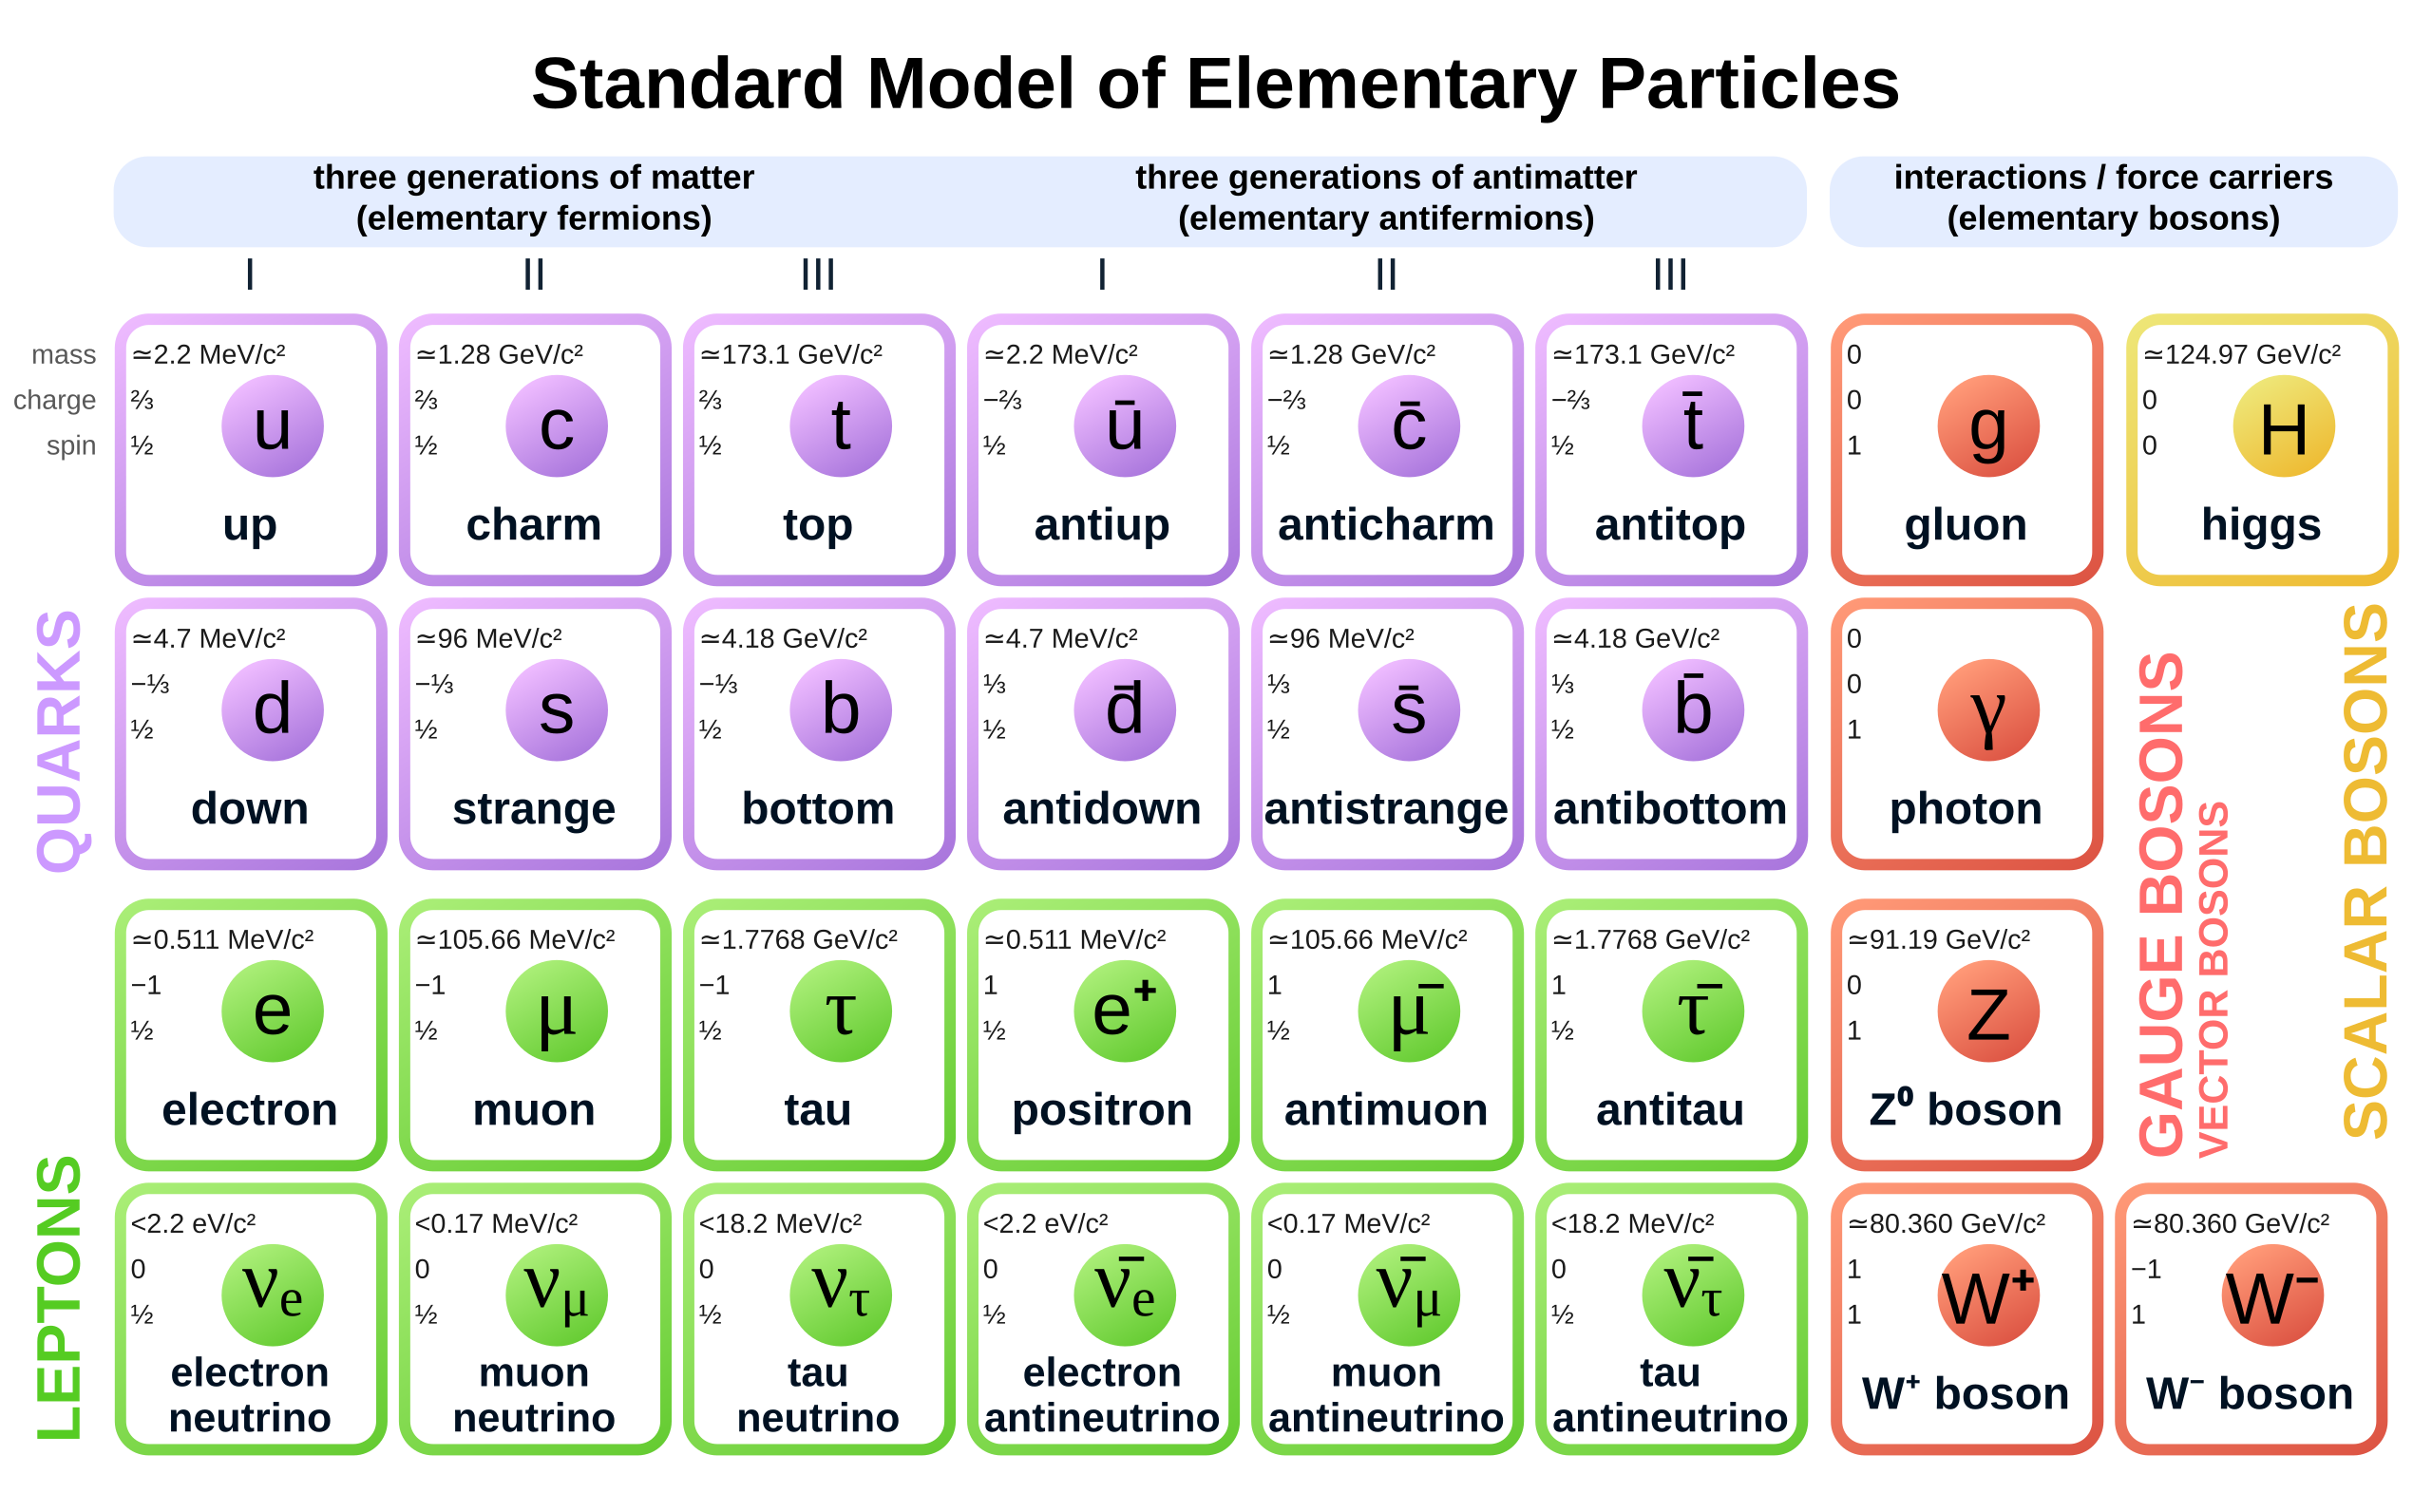
\includegraphics[width=0.8\textwidth]{figures/theory/theory_standard_model.png}
    \caption{Depicted is the visual version of the Standard Model. The elementary particles are grouped via fermions and bosons. Fermions are further divided into quarks and leptons. The bosons are divided into gauge bosons and the Higgs boson. Additionally, the corresponding antiparticles are shown. Taken from~\cite{theory_sm_figure}.}\label{fig:standard_model}
\end{figure}
% \section{Mathematical Introduction}\label{sec:theory_mathematical_intro}
% % To understand the mathematical foundation that the Standard Model is built upon, it is necessary to start with the basic mathematical principles that the Standard Model is based on. In this Section we will introduce what a group is, and how groups describe symmetries. Then, we will discuss Lie groups, which define the symmetries of the Standard Model. Finally, we will discuss gauge symmetries and the U(1), SU(2), and SU(3) groups that are used in the Standard Model. 
% This section begins by introducing the concept of a group, which provides a mathematical description of symmetry. We then move on to Lie groups which define the symmetries of the Standard Model. Finally, we present the groups U(1), SU(2), and SU(3) as examples of Lie groups that will later appear in physical contexts. Their specific roles in quantum field theories will be discussed in detail in Sections~\ref{sec:theory_qed},~\ref{sec:theory_qcd} and~\ref{sec:theory_ew}.Sections~\ref{sec:theory_qed},~\ref{sec:theory_qcd} and~\ref{sec:theory_ew}.
This section provides a brief introduction to the mathematical concepts essential for deriving the Standard Model Lagrangian, including groups, Lie groups, and gauge symmetries. While the mathematical formalism is not the focus of this thesis, it is necessary for a deeper understanding of the Standard Model.
\section{Groups of The Standard Model}\label{sec:theory_groups}
In the derivation of the Standard Model Lagrangian, group theory plays an essential role. A group $G$ is defined as a set of elements with a binary operation $\ast$ that follow four axioms:
\begin{enumerate}
  \item G is closed under $\ast$, meaning $\forall a, b \in G, \; a \ast b \in G$  
  \item The operation $\ast$ is associative, meaning $\forall a, b, c \in G, \; (a \ast b) \ast c = a \ast (b \ast c)$.
  \item Each element has an identity, meaning $\exists I \in G$ so that $\forall a \in G, \; I \ast a = a \ast I = a$.
  \item Each element has an inverse, meaning $\forall a \in G, \; \exists b \in G$ so that $a \ast b = b \ast a = I$.
\end{enumerate}
Additionally, a group is said to be abelian if it's elements are commutative under $\ast$. 

In physics, symmetry groups are used to describe transformations that leave physical systems unchanged. The Standard Model is built on a special class of symmetry groups known as Lie groups, which is a continuous group whose elements can be parameterized by smooth transformations. The simplest example is $\mathrm{U}(1)$, the group of all $1 \times 1$ unitary matrices. This group is abelian and corresponds to phase rotations in the complex plane. In Section~\ref{sec:theory_qed} this group will play an important role in the formalism of quantum electrodynamics. 

Another important class of Lie groups are the special unitary groups, denoted by $\mathrm{SU}(N)$. These are a non-abelian group, consisting of all $N \times N$ unitary matrices with determinant 1. Only two such groups are relevant for the Standard Model: $\mathrm{SU}(3)$ (Section~\ref{sec:theory_qcd}) and $\mathrm{SU}(2)$ (Section~\ref{sec:theory_ew}).

These symmetry groups form the mathematical foundation for the structure of the Standard Model: $\mathrm{U}(1)$ for electromagnetism, $\mathrm{SU}(2)$ for the weak interaction, and $\mathrm{SU}(3)$ for the strong interaction. Together, they define the group $\mathrm{SU}(3)C \times \mathrm{SU}(2)L \times \mathrm{U}(1)Y$, which determines how elementary particles interact. The Standard Model Lagrangian is given by the following:
\begin{equation}
  \mathcal{L}_{\mathrm{SM}} = \mathcal{L}_{\mathrm{strong}} + \mathcal{L}_{\mathrm{EW}} + \mathcal{L}_{\mathrm{Yukawa}} + \mathcal{L}_{\mathrm{Higgs}}
  \label{eq:sm_lagrangian}
\end{equation}
which encapsulates these symmetries and will be explored in detail in the sections that follow.

\section{Quantum Electrodynamics}\label{sec:theory_qed}
Quantum electrodyanmics (QED) is the description of electromagnetic interaction between charged particles and photons as a relativistic quantum field theory (QFT). It is an abelian gauge theory with the symmetry group $\mathrm{U}(1)$. As previously mentioned, the $\mathrm{U}(1)$ symmetry group corresponds to phase rotations in the complex plane and represent a global symmetry. The full Lagrangian density for charged Dirac fermions interacting with the EM field is given by
\begin{equation}
  \mathcal{L} = \bar{\psi}(i\gamma^{\mu}\partial_{\mu} - m)\psi 
  \label{eq:qed_dirac_lagrangian}
\end{equation}
with fermion field $\psi$, mass $m$, and the Dirac matrices $\gamma^{\mu}$. Since global symmetries correspond to conservation laws via Noether's theorem, one might wonder whether these symmetries can be extended to local transformations as well. Consider a field $\psi$ undergoing a local transformation $\chi(x)$
\begin{equation}
  \psi(x) \to \psi(x)e^{i q\chi(x)} 
  \label{eq:qed_local_symmetry}
\end{equation}
the Lagrangian transforms as
\begin{equation}
  \mathcal{L}' = \mathcal{L} + \bar{\psi} iq\gamma^{\mu}\partial_{\mu}\chi(x) \psi
  \label{eq:qed_local_lagrangian}
\end{equation}
but this is not invariant under the local transformation as we are left with an extra term. To remedy this, we must introduce a gauge field $A_{\mu}$, which transforms as
\begin{equation}
  A_{\mu} \to A_{\mu} + \partial_{\mu}\chi(x)
  \label{eq:qed_gauge_transformation}
\end{equation}
and we must replace that partial derivative in the Lagrangian with a covariant derivative defined as
\begin{equation}
  D_{\mu} = \partial_{\mu} + iqA_{\mu}
  \label{eq:qed_covariant_derivative}
\end{equation}
ensuring that the Lagrangian is invariant under local transformations. The Lagrangian density can then be written as
\begin{align}
  \mathcal{L} 
  &= \bar{\psi}(i\gamma^{\mu}D_{\mu} - m)\psi \nonumber \\
  &= \bar{\psi}(i\gamma^{\mu}\partial_{\mu} - m)\psi + q\bar{\psi}\gamma^{\mu}A_{\mu}\psi 
  \label{eq:qed_lagrangian_no_kinetic}
\end{align}
which is now fully invariant under local $\mathrm{U}(1)$ transformations. The introduction of the gauge field has naturally generated an interaction term between the fermion and gauge field, as seen in Equation~\ref{eq:qed_lagrangian_no_kinetic}. To complete QED, we must include the kinetic terms for the gauge field. Naively, one would think that this term is just ${(\partial_{\mu}A_{\nu})}^{2}$ but this breaks the gauge invariance. Instead, we introduce the electromagnetic field strength tensor $F_{\mu\nu}$, defined as
\begin{equation}
  F_{\mu\nu} = \partial_{\mu}A_{\nu} - \partial_{\nu}A_{\mu}
  \label{eq:qed_field_strength_tensor}
\end{equation}
which is invariant under the gauge transformation. The kinetic term for the gauge field is then given by
\begin{equation}
  \mathcal{L}_{\mathrm{EM}} = - \frac{1}{4}F^{\mu\nu}F_{\mu\nu}
  \label{eq:qed_em_free_lagrangian}
\end{equation}
The full Lagrangian density for QED becomes
\begin{equation}
  \mathcal{L}_{\mathrm{QED}} = \bar{\psi}(i\gamma^{\mu}D_{\mu} - m)\psi - \frac{1}{4}F^{\mu\nu}F_{\mu\nu}
  \label{eq:qed_lagrangian}
\end{equation}
where the last term corresponds to the mass of the gauge field. However, this term breaks the local gauge invariance, therefore, the mass of the gauge field must vanish. 
\begin{equation}
  \mathcal{L}_{\mathrm{QED}} = \bar{\psi}(i\gamma^{\mu}D_{\mu} - m)\psi - \frac{1}{4}F^{\mu\nu}F_{\mu\nu}
  \label{eq:qed_lagrangian_final}
\end{equation}
In this context, we interpret the gauge field $A_{\mu}$ as the massless photon field with coupling strength $q$.


\section{Quantum Chromodynamics}\label{sec:theory_qcd}
Quantum chromodynamics (QCD) is the relativistic quantum field theory that describes the strong interaction between quarks and gluons. Quarks are electrically charged fermions that also carry color charge, analogous to the electric charge in QED\@. Gluons are electrically neutral particles that consist of a color and anticolor charge. There are three color charges: red, green, and blue ($r$, $g$, $b$) as well as three corresponding anticolor charges: anti-red, anti-green, and anti-blue ($\bar{r}$, $\bar{g}$, $\bar{b}$). 

QCD is a non-Abelian gauge theory based on the symmetry group $\mathrm{SU}(3)$, representing phase transformations of the quark color fields. Analogous to QED, we begin with the free Dirac Lagrangian density for quarks:
\begin{equation}
  \mathcal{L}_{\mathrm{QCD}} = \bar{q}(i\gamma^{\mu}\partial_{\mu} - m)q
  \label{eq:qcd_free_lagrangian}
\end{equation}
with mass $m$, and $q$ the quark color triplet field
\begin{equation}
  q = \begin{pmatrix}
    q_{r} \\
    q_{g} \\
    q_{b}
  \end{pmatrix}
  \label{eq:qcd_quark_field}
\end{equation}
with each component $q_{c}$ being a Dirac spinor. The Langrangian density in Equation~\ref{eq:qcd_free_lagrangian} is invariant under global $\mathrm{SU}(3)$ transformations To promote this symmetry to a local one we consider local phase transformations of the form
\begin{equation}
  q(x) \to Uq(x) \equiv e^{i\chi_{a}(x)T_{a}}q(x)
  \label{eq:qcd_local_symmetry}
\end{equation}
where $U(x) \in \mathrm{SU}(3)$, $\chi_{a}(x)$ are the local parameters of the transformation, and $T_{a}$ are the generators of the $\mathrm{SU}(3)$ group, the Gell-Mann matrices. These generators are a set of $8$ $3 \times 3$ hermitian matrices that satisfy the commutation relations
\begin{equation}
  [T_{a}, T_{b}] = i f_{abc}T_{c}
  \label{eq:qcd_commutation_relation}
\end{equation}
with real structure constants $f_{abc}$. Under local $\mathrm{SU}(3)$ transformations, the derivative term in Equation~\ref{eq:qcd_free_lagrangian}, is not invariant. To restore the local gauge invariance, we introduce eight gauge fields $G_{\mu}^{a}$, one for each generator $T_{a}$, which transform as
\begin{equation}
  G_{\mu}^{a} \to G_{\mu}^{a} - \frac{1}{g} \partial_{\mu}\chi_{a} - f_{abc}\chi_{b}G_{\mu}^{c},
\end{equation}
and we define the covariant derivative as
\begin{equation}
  D_{\mu} = \partial_{\mu} + ig T_{a}G_{\mu}^{a}.
  \label{eq:qcd_covariant_derivative}
\end{equation}
Finally, we must include the kinetic term for each of the gauge fields as we did for QED\@. The strong field strength tensor is defined as
\begin{equation}
  G_{\mu\nu}^{a} = \partial_{\mu}G_{\nu}^{a} - \partial_{\nu}G_{\mu}^{a} + g f_{abc}G_{\mu}^{b}G_{\nu}^{c}
  \label{eq:qcd_field_strength_tensor}
\end{equation}
with the resulting Lagrangian density given by
\begin{align}
  \mathcal{L}_{\mathrm{QCD}} &= \bar{q}(i\gamma^{\mu}D_{\mu} - m)q - \frac{1}{4}G_{\mu\nu}^{a}G^{\mu\nu a} + \frac{1}{2}m^2G_{\mu}^{a}G^{\mu a} \nonumber \nonumber \\
  &= \bar{q}(i\gamma^{\mu}\partial_{\mu} - m)q + g(\bar{q}T_{a}\gamma^{\mu}q)G_{\mu}^{a} - \frac{1}{4}G_{\mu\nu}^{a}G_{a}^{\mu\nu} + \frac{1}{2}mG_{\mu\nu}^{a}G_{a}^{\mu\nu}.
  \label{eq:qcd_lagrangian}
\end{align}
However, the gauge field mass term breaks the gauge invariance, therefore the mass of all the gauge fields must vanish. The final Lagrangian density for QCD is given by
\begin{equation}
  \mathcal{L}_{\mathrm{QCD}} = \bar{q}(i\gamma^{\mu}\partial_{\mu} - m)q + g(\bar{q}T_{a}\gamma^{\mu}q)G_{\mu}^{a} - \frac{1}{4}G_{\mu\nu}^{a}G_{a}^{\mu\nu}
  \label{eq:qcd_lagrangian_final}
\end{equation}
where $g$ is the coupling constant of the strong interaction, analogous to the electric charge in QED\@. The strong field strength tensor $G_{\mu\nu}^{a}$ has a remarkable difference from the electromagnetic field strength tensor in QED\@. The non-Abelian nature of the gauge group $\mathrm{SU}(3)$ leads to self-interactions between the gluons, which is absent in QED\@. This self-interacticon results interactions between three or four gluons, which is a unique feature of QCD not present in QED\@.

These self-interactions are responsible for two phenomenon that appear in QCD, asymptotic freedom and confinement. Asymptotic freedom refers to the phenomenon where the effective strong coupling is weaker at high energies or short distances. In this regime, quarks and gluons interact only weakly and can be treated as nearly free particles. This property explains why many gluon-induced QCD processes become prominent at high-energy colliders. In contrast, at low energies or large distances, the strong coupling increases due to the running of the coupling constant, ultimately leading to confinement. In this regime, the force between colored particles becomes so strong that it is energetically more favorable to create a quark-antiquark pair from the vacuum than to separate two color charges. As a result, colored particles such as quarks and gluons are never observed in isolation, but are permanently confined within color-neutral bound states known as hadrons.

\section{Electroweak Theory}\label{sec:theory_ew}
Describing the weak interaction is more complex than QED or QCD due to several unique features. The theory needs to describe several different type fermions (quarks, leptons) and treat left- and right-handed fields differently. Specifically, only left-handed fermions participate in weak interactions and must appear in doublets, while right-handed fermions are singlets. Additionally, the theory needs to produce a massless photon but also produces three massive gauge bosons associated to the weak interaction. 

To accommodate the doublet structure required for the weak interaction the natural choice for a symmetry group is $\mathrm{SU}(2)$. To incorporate the electromagnetic interaction as well, an additional $\mathrm{U}(1)$ group is required, as described in Section~\ref{sec:theory_qed}. The symmetry group chosen to define the electroweak interaction is $\mathrm{SU}{(2)}_{L} \otimes \mathrm{U}{(1)}_{Y}$ where $L$ indicates that $\mathrm{SU}(2)$ only acts on left-handed fields, and $Y$ denotes the weak hypercharge associated with $\mathrm{U}(1)$. 

We begin by introducing the left-handed doublets and right-handed singlets. For leptons, this is defined as
\begin{equation}
  \psi_{L} = \begin{pmatrix}
    \nu_{\ell} \\
    \ell^{-}
  \end{pmatrix}_{L}, \quad
  \psi_{R} = \ell_{R}, \bar{\nu}_{\ell R}
  \label{eq:ew_lepton_fields}
\end{equation}
where $\ell$ is any charged lepton and $\nu_{\ell}$ the corresponding neutrino. For quarks we define
\begin{equation}
  \psi_{L} = \begin{pmatrix}
    q \\
    q'
  \end{pmatrix}_{L}, \quad
  \psi_{R} = q_{R}, q'_{R}
  \label{eq:ew_quark_fields}
\end{equation}
where $q$ is an up-type quark and $q'$ corresponding down-type quark. 

Following the prescription developed for QED and QCD, we consider the free Lagrangian
\begin{equation}
  \mathcal{L}_{\mathrm{EW}} = \bar{\psi}_{L}(i\gamma^{\mu}\partial_{\mu} - m)\psi_{L} + \bar{\psi}_{R}(i\gamma^{\mu}\partial_{\mu} - m)\psi_{R}
  \label{eq:ew_free_lagrangian}
\end{equation}
where $m$ is the mass of the fermion. Unlike the previous sections, this Lagrangian is separated into left- and right-handed components to reflect the structure of the weak interaction. As before, this Lagrangian is invariant under global transformations but we wish to promote this invariance to a local one. The local gauge transformations are
\begin{equation}
  \psi_{L} \to U_{L}\psi_{L}, \quad
  \psi_{R} \to U_{R}\psi_{R}
  \label{eq:ew_local_symmetry}
\end{equation}
with
\begin{equation}
  U_{L} = e^{i(y_{L}\chi(x) + \frac{\sigma_{i}}{2}\alpha^{i}(x))}, \quad
  U_{R} = e^{i(y_{R}\chi(x))}
  \label{eq:ew_local_transformation}
\end{equation}
where $y_{L}$ and $y_{R}$ are the hypercharges of the left- and right-handed fields, and $\sigma_{i}$ the Pauli matrices, which serve as the $\mathrm{SU}(2)$ generators. 

To maintain local gauge invariance, three gauge fields $W_{\mu}^{i}$ are introduced for the $\mathrm{SU}(2)$ group and one gauge field $B_{\mu}$ for the $\mathrm{U}(1)$ group. The corresponding covariant derivatives are defined as
\begin{align}
  D_{\mu}\psi_{L} &= (\partial_{\mu} - ig\frac{\sigma_{i}}{2}W^{i}_{\mu}(x) - ig'Y_{L}B_{\mu}(x))\psi_{L}, \\ \quad 
  D_{\mu}\psi_{R} &= (\partial_{\mu} - ig'Y_{R}B_{\mu}(x))\psi_{R}
  \label{eq:ew_covariant_derivative} 
\end{align}
where $g$ and $g'$ are the coupling constants of the $\mathrm{SU}(2)$ and $\mathrm{U}(1)$ groups respectively.

By demanding local gauge invariance our Lagrangian from Equation~\ref{eq:ew_free_lagrangian} becomes 
\begin{equation}
  \mathcal{L} \to g\bar{\psi}_{L}\gamma^{\mu}\frac{\sigma_{i}}{2}W_{\mu}^{i}\psi_{L} + g'B_{\mu}y_{L}\bar{\psi}_{L}\gamma^{\mu}\psi_{L} + g'B_{\mu}y_{R}\bar{\psi}_{R}\gamma^{\mu}\psi_{R}.
  \label{eq:ew_lagrangian}
\end{equation}
To write this more traditionally, we express the $\mathrm{SU}(2)$ term explicitly, where
\begin{equation}
  \frac{\sigma^{i}}{2}W_{\mu}^{i} = \frac{1}{\sqrt{2}}\begin{pmatrix}
    \sqrt{2}W_{\mu}^{3} &  W_{\mu}^{+} \\
    W_{\mu}^{-} & -\sqrt{2}W_{\mu}^{3}
  \end{pmatrix}
\end{equation}
with $W_{\mu}^{\pm} = \frac{1}{\sqrt{2}}(W_{\mu}^{1} \mp iW_{\mu}^{2})$ and $W_{\mu}^{3}$ the neutral $\mathrm{SU}(2)$ gauge field. The first term becomes a charged-current interaction and takes the form
\begin{equation}
  \mathcal{L}_{\mathrm{CC}} = \frac{g}{2\sqrt{2}}\{W^{+}[\bar{q}\gamma^{\mu}(1-\gamma_{5})q' + \bar{\nu}_{\ell}\gamma^{\mu}(1 - \gamma_{5})\ell] + \mathrm{h.c.}\}
  \label{eq:ew_cc_lagrangian}
\end{equation}
which gives rise to the charged weak interactions mediated by the $W^{\pm}$ bosons. These interactions couple the upper and lower components of the weak doublet, and are responsible for lepton flavor transitions, and quark flavor-changing interactions. 

In addition to the charged-current term, there is another term involving two neutral gauge fields $W^{3}_{\mu}$ and $B_{\mu}$. Naturally, we would like to identify these as $\gamma$ and $Z$ bosons but this is not possible. The key problem is the electromagnetic interaction where the photon must couple identically to left- and right-handed fermions. In the electroweak framework, $W^{3}_{\mu}$ and $B_{\mu}$ couple differently to left- and right-handed fermions. This asymmetry is essential for the weak interaction since it is a parity violating interaction, but presents a problem for constructing a parity-conserving electromagnetic interaction. The $B_{\mu}$ field couples to fermions with a strength proportional to their hypercharge, which differs depending on chiralty. 

Since $W^{3}_{\mu}$ and $B_{\mu}$ are neutral, we can try constructing a linear combination of the two fields
\begin{equation}
  \begin{pmatrix}
    W^{3}_{\mu}\\
    B_{\mu}
  \end{pmatrix} = \begin{pmatrix}
    \cos\theta_{W} & \sin\theta_{W} \\
    -\sin\theta_{W} & \cos\theta_{W}
  \end{pmatrix}
  \begin{pmatrix}
    Z_{\mu} \\
    A_{\mu}
  \end{pmatrix}
  \label{eq:ew_mixing}
\end{equation}
where $\theta_{W}$ is the weak mixing angle. The neutral charged Lagrangian can then be derived and is given by
\begin{equation}
  \mathcal{L}_{\mathrm{NC}} = \sum_{j}\bar{\psi}_{j}\gamma^{\mu} \{A_{\mu}[g\frac{\sigma_{3}}{2}\sin{\theta_{W}} + g'\cos{\theta_{W}}] + Z_{\mu}[g\frac{\sigma_{3}}{2}\cos{\theta_{W} - g'y_{j}\sin{\theta_{W}}}] \} \psi_{j}.
  \label{eq:ew_nc_lagrangian}
\end{equation}
To extract QED from the $A_{\mu}$ term, two conditions need to be imposed. First we need to set $g\sin{\theta_{W}} = g'\cos{\theta_{W}} = e$ as this relates the $\mathrm{SU}{(2)}_{L}$ and $\mathrm{U}(1)$ couplings to the electromagnetic coupling. Secondly, we require that $Y = Q - T_{3}$ which fixes fermion hypercharges in terms of their electric charge and weak isospin. Which these conditions the Lagrangian can now be written as
\begin{equation}
  \mathcal{L}_{NC} = \mathcal{L}_{\mathrm{QED}} + \mathcal{L}_{\mathrm{NC}}^{Z} 
\end{equation}
where $\mathcal{L}_{\mathrm{QED}}$ is the QED Lagrangian defined in Section~\ref{sec:theory_qed} and $\mathcal{L}_{\mathrm{NC}}^{Z}$ is the neutral current Lagrangian given by
\begin{equation}
  \mathcal{L}_{\mathrm{NC}}^{Z} = \frac{e}{\sin{\theta_{W}}\cos{\theta_{W}}} \left(\sum_{j}\bar{\psi}_{j}\gamma^{\mu}(T_{3} - \sin^2{\theta_{W}}Q_{j})\psi_{j}\right)Z_{\mu}
  \label{eq:ew_nc_lagrangian_z}
\end{equation}
Finally, all that is left is to introduce the kinematic term for the gauge bosons. These are built in similar ways to the previous two sections using field strength tensors which are defined as
\begin{align}
  W_{\mu\nu}^{i} &= \partial_{\mu}W_{\nu}^{i} - \partial_{\nu}W_{\mu}^{i} + g\epsilon_{ijk}W_{\mu}^{j}W_{\nu}^{k}, \\
  B_{\mu\nu} &= \partial_{\mu}B_{\nu} - \partial_{\nu}B_{\mu}
\end{align}
where $\epsilon^{ijk}$ is the Levi-Civita symbol. The kinetic term for the gauge bosons is then given by
\begin{equation}
  \mathcal{L}_{\mathrm{kin}} = -\frac{1}{4}W_{\mu\nu}^{i}W^{\mu\nu i} - \frac{1}{4}B_{\mu\nu}B^{\mu\nu}.
  \label{eq:ew_kinetic_lagrangian}
\end{equation}
The final electroweak Lagrangian is given by
\begin{equation}
  \mathcal{L}_{\mathrm{EW}} = \mathcal{L}_{\mathrm{CC}} + \mathcal{L}_{\mathrm{NC}} + \mathcal{L}_{\mathrm{kin}}.
  \label{eq:ew_lagrangian_final}
\end{equation}
With this derivation, nearly all of the original goals of the electroweak theory have been met. However, all four gauge bosons remain massless, in contradiction with experimental observations that the weak interaction must occur through a massive force carrier due to the short range nature. This implies that the electroweak symmetry must be broken somehow. The solution to this problem is the Higgs mechanism, which is discussed in the next section.



\section{Higgs Mechanism}\label{sec:theory_higgs_mechanism}
The Higgs mechanism is the mechanism that allows the massless gauge bosons to acquire mass while preserving the $\mathrm{SU}{(2)}_{L} \otimes \mathrm{U}{(1)}_{Y}$ symmetry. To achieve this, we start by introducing a new $\mathrm{SU}(2)$ doublet of complex scalar fields,
\begin{equation}
  \phi = \begin{pmatrix}
    \phi^{+} \\
    \phi^{0}
  \end{pmatrix}
  \label{eq:higgs_doublet}
\end{equation}
where $\phi^{+}$ is a charged scalar field $\phi^{+} = \frac{1}{\sqrt{2}}(\phi_{1} + i \phi_{2})$ and $\phi^{0}$ is a neutral scalar field $\phi^{0} = \frac{1}{\sqrt{2}}(\phi_{3} + i \phi_{4})$, as well as a new term for the Standard Model Lagrangian,
\begin{equation}
  \mathcal{L}_{\mathrm{Higgs}} = {(D_{\mu}\phi)}^{\dagger}(D^{\mu}\phi) - V(\phi)
  \label{eq:higgs_lagrangian}
\end{equation}
where $D_{\mu}$ is the covariant derivative and $V(\phi)$ is known as the Higgs potential and takes the form of $V(\phi) = \mu^{2}\phi^{\dagger}\phi + \lambda{(\phi^{\dagger}\phi)}^{2}$. To extract physical masses, we can study the Higgs potential. The potential can behavior in two distinct ways depending on the sign of $\mu^{2}$:
\begin{itemize}
  \item For $\mu^{2} > 0$, the potential only has the trivial solution of $\phi = 0$, and would describe a scalar particle with mass $\mu$ and coupling $h$. 
  \item More interestingly, for $\mu^{2} < 0$ (Figure~\ref{fig:theory_higgs_potential}), the potential has a non-trivial minimum at $\phi^{0} = \sqrt{\frac{-\mu^{2}}{2\lambda}} = \frac{v}{\sqrt{2}}$, and due to the $\mathrm{U}(1)$ phase invariance, there are infinitely many of these solutions, and are referred to as the vacuum expectation value (VEV) of the Higgs field.
\end{itemize}

\begin{figure}
  \centering
  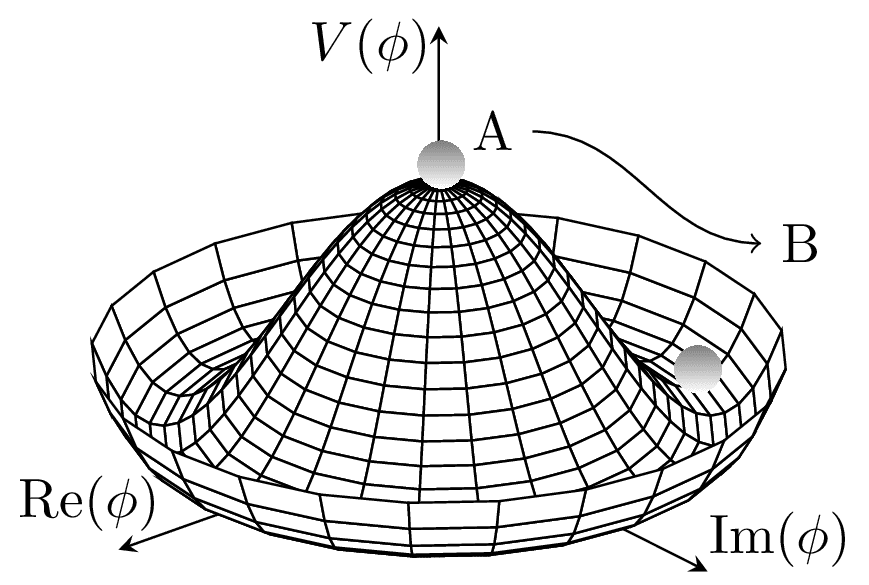
\includegraphics[width=0.5\textwidth]{figures/theory/theory_higgs_potential.png}
  \caption{The Higgs potential $V(\phi)$ as a function of the Higgs field $\phi$. The potential has a non-trivial minimum at $\phi^{0} = \sqrt{\frac{-\mu^{2}}{2\lambda}} = \frac{v}{\sqrt{2}}$ for $\mu^{2} < 0$. Taken from~\cite{riebesell_higgs_potential_2022}.}\label{fig:theory_higgs_potential}
\end{figure}

Without loss of generality, we can pick a particular vacuum solution as the ground state, thereby spontaneously breaking the original $\mathrm{SU}{(2)}_{L} \otimes \mathrm{U}{(1)}_{Y}$ symmetry down to the unbroken $\mathrm{U}{(1)}_{em}$ symmetry, which remains a true symmetry of the vacuum. To expand the Higgs field around the vacuum, we choose a specific minimum by setting $\phi_{1}=\phi_{2}=\phi_{4} = 0$ and $\phi_{3} = v$. However, there still remains fluctuations that are associated with the broken symmetry generators. These fluctuations can be parameterized by Goldstone bosons, $\theta^{i}(x)$, which appear in the field expansion as phase rotations. The expansion of the Higgs field around the VEV is
\begin{equation}
  \phi = \begin{pmatrix}
    0 \\
    \frac{v + h(x)}{\sqrt{2}}
  \end{pmatrix} e^{i\frac{\sigma_{i}}{2}\theta^{i}(x)}.
  \label{eq:higgs_expansion}
\end{equation}
We can now plug this into Equation~\ref{eq:ew_covariant_derivative} and choose the unitary gauge $\theta^{i}(x) = 0$, we see that the kinetic piece of the Lagrangian becomes
\begin{equation}
  {(D_{\mu}\phi)}^{\dagger}D^{\mu}\phi \rightarrow \frac{1}{2}\partial_{\mu}h\partial^{\mu}h + {(v+h)}^{2}\{\frac{g^{2}}{4}W_{\mu}^{\dagger}W^{\mu} + \frac{g^{2}}{8\cos^2{\theta_{W}}}Z_{\mu}Z^{\mu}   \}.
\end{equation}
The spontaneous breaking of the $\mathrm{SU}{(2)}_{L} \otimes \mathrm{U}{(1)}_{Y}$ symmetry lead to the emergence of three massless Goldstone bosons, corresponding to the three broken generators of the symmetry. The presence of these massless scalars appears to be problematic, however, by substituting the Higgs field expansion into the kinetic term of Equation~\ref{eq:higgs_lagrangian} and working in the unitary gauge, these Goldstone bosons are effectively removed. In doing so, we find that the $W^\pm$ and $Z$ bosons acquire mass, while the photon remains massless, consistent with the fact that the unbroken $\mathrm{U}(1)$ symmetry is preserved. The masses of the $W^\pm$ and $Z$ bosons are given by
\begin{align}
  m_{W} &= \frac{1}{2}g v, \\
  m_{Z} &= \frac{gv}{2\cos{\theta_{W}}}.
  \label{eq:higgs_masses}
\end{align}

With the gauge bosons now massive, we can acquire the mass terms for the fermions in a similar fashion. We can consider the fermion mass term
\begin{equation}
  \mathcal{L}_{Fermion,mass} = -m\psi\bar{\psi} = -m(\bar{\psi}_{L}\psi_{R} + \bar{\psi}_{R}\psi_{L})
\end{equation}
where $\psi$ is the fermion field. This type of mass term is not allowed due to it breaking the gauge symmetry. However, since we have introduced another scalar doublet into the model we can write a Yukawa interaction term like
\begin{equation}
  \mathcal{L}_{Yukawa} = c\bar{\psi}_{L}\phi\psi_{R} + \mathrm{h.c.}.
  \label{eq:higgs_yukawa}
\end{equation}
Using the fermion fields from Equations~\ref{eq:ew_lepton_fields} and~\ref{eq:ew_quark_fields}, we can write the Yukawa interaction term as 
\begin{equation}
  \mathcal{L}_{Yukawa} = c_{q'} {(\bar{q}, \bar{q}')}_{L}\begin{pmatrix}
    \phi^{+} \\
    \phi^{0}
  \end{pmatrix}
  q_{R}' + c_{q}{(\bar{q}, \bar{q}')}_{L}\begin{pmatrix}
    \phi^{0*} \\
    -\phi^{-}
  \end{pmatrix}
  q_{R} + c_{\ell}{(\bar{\ell}, \bar{\nu}_{\ell})_{L}}\begin{pmatrix}
    \phi^{+} \\
    \phi^{0}
  \end{pmatrix}
  \ell_{R} + h.c.
\end{equation}
where $c_{q}$, $c_{q'}$, and $c_{\ell}$ are the Yukawa couplings. After symmetry breaking and choosing the unitary gauge, the Yukawa interaction simplifies to
\begin{equation}
  \mathcal{L}_{Yukawa} = \frac{1}{\sqrt{2}}(v+h)\{c_{q'}\bar{q}'q' + c_{q}\bar{q}q + c_{\ell}\bar{\ell}\ell\}.
\end{equation}
From this, it is clear that the Standard Model does not predict the values of fermion masses since they depend on free parameters that must be determined experimentally. Additionally, it demonstrates that the fermion masses are dependent on the VEV of the Higgs field, a direct consequence of the symmetry breaking. 

The Yukawa Lagrangian assumes that each quark flavor can only transform into their corresponding `up' or `down' type quark of opposite sign. However, this assumption is not consistent with experimental observations where, for example, a $u$ quark has been found to become a $\bar{s}$ quark. This discrepancy is resolved by introducing the Cabibo-Kobayashi-Maskawa (CKM) matrix, which accounts for the fact that the weak interaction eigenstates are not the same as the mass eigenstates. The CKM matrix is a $3\times3$ unitary matrix that relates the weak interaction eigenstates to their mass eigenstates via
\begin{equation}
  \begin{pmatrix}
    d' \\
    s' \\
    b' \\
  \end{pmatrix}
  = \begin{pmatrix}
    V_{ud} & V_{us} & V_{ub} \\
    V_{cd} & V_{cs} & V_{cb} \\
    V_{td} & V_{ts} & V_{tb}
  \end{pmatrix}
  \begin{pmatrix}
    d \\
    s \\
    b \\
  \end{pmatrix}
  \label{eq:ckm_matrix}
\end{equation}
where the off-diagonal terms represent the mixing between the different quark flavors. These values are not predicted by the Standard Model and must be determined experimentally. 

We conclude by returning to the Higgs Lagrangian defined in Equation~\ref{eq:higgs_lagrangian}. After symmetry breaking and choosing the unitary gauge, the Lagrangian becomes
\begin{equation}
  \mathcal{L}_{\mathrm{Higgs}} = \frac{1}{2}\partial^{\mu}h\partial_{\mu}h - \mu^{2}h^{2} - \lambda v h^{3} - \frac{1}{4}\lambda h^{4}
\end{equation}
where the $h$ field is the Higgs boson that has mass $\sqrt{2\lambda}v$. From the Higgs Lagrangian, it is evident that the Higgs boson couples to itself through two-, three-, and four-point interaction vertices, corresponding to $hhh$ and $hhhh$ self-couplings. With this, all main ingredients of the SM Lagrangian have been introduced, we can now proceed to the Higgs boson production modes and decay channels.
\section{Higgs Boson Couplings and Decays}\label{sec:theory_higgs_decay}
The discovery of the Higgs boson completed the Standard Model in 2012 and confirmed the Higgs mechanism for the electroweak symmetry breaking and mass generation. Beyond this, we are able to measure its couplings to other particles as well as its decay modes.

\begin{figure}[pht]
  \centering
  \subfloat[Higgs coupling constants vs particle mass, Taken from~\cite{LHC_Higgs_handbook}]{
    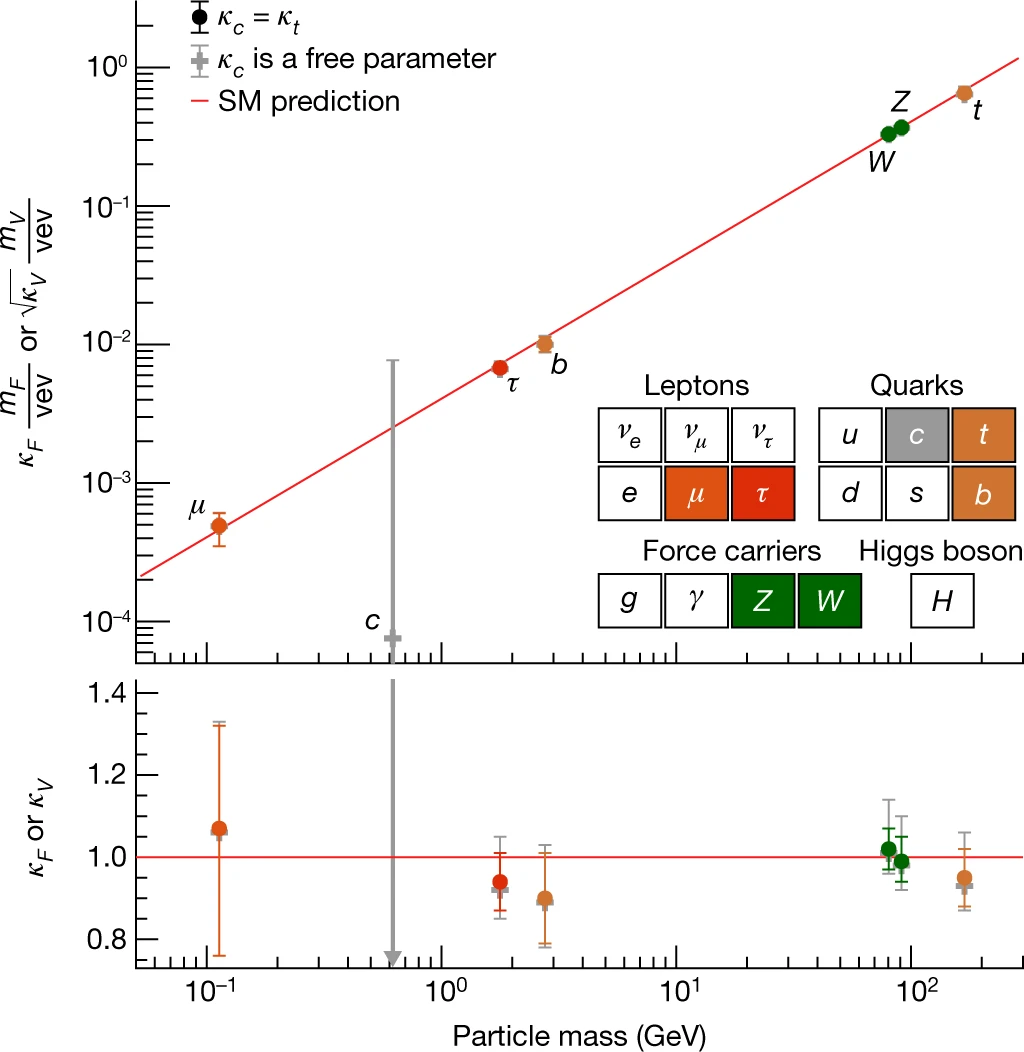
\includegraphics[width=0.45\textwidth]{figures/theory/theory_coupling_strengths.png}\label{fig:coupling_vs_mass}
  }\hspace{0.01\textwidth}
  \subfloat[Higgs boson branching ratios vs mass, Taken from~\cite{ATLAS_Open_Data}]{
    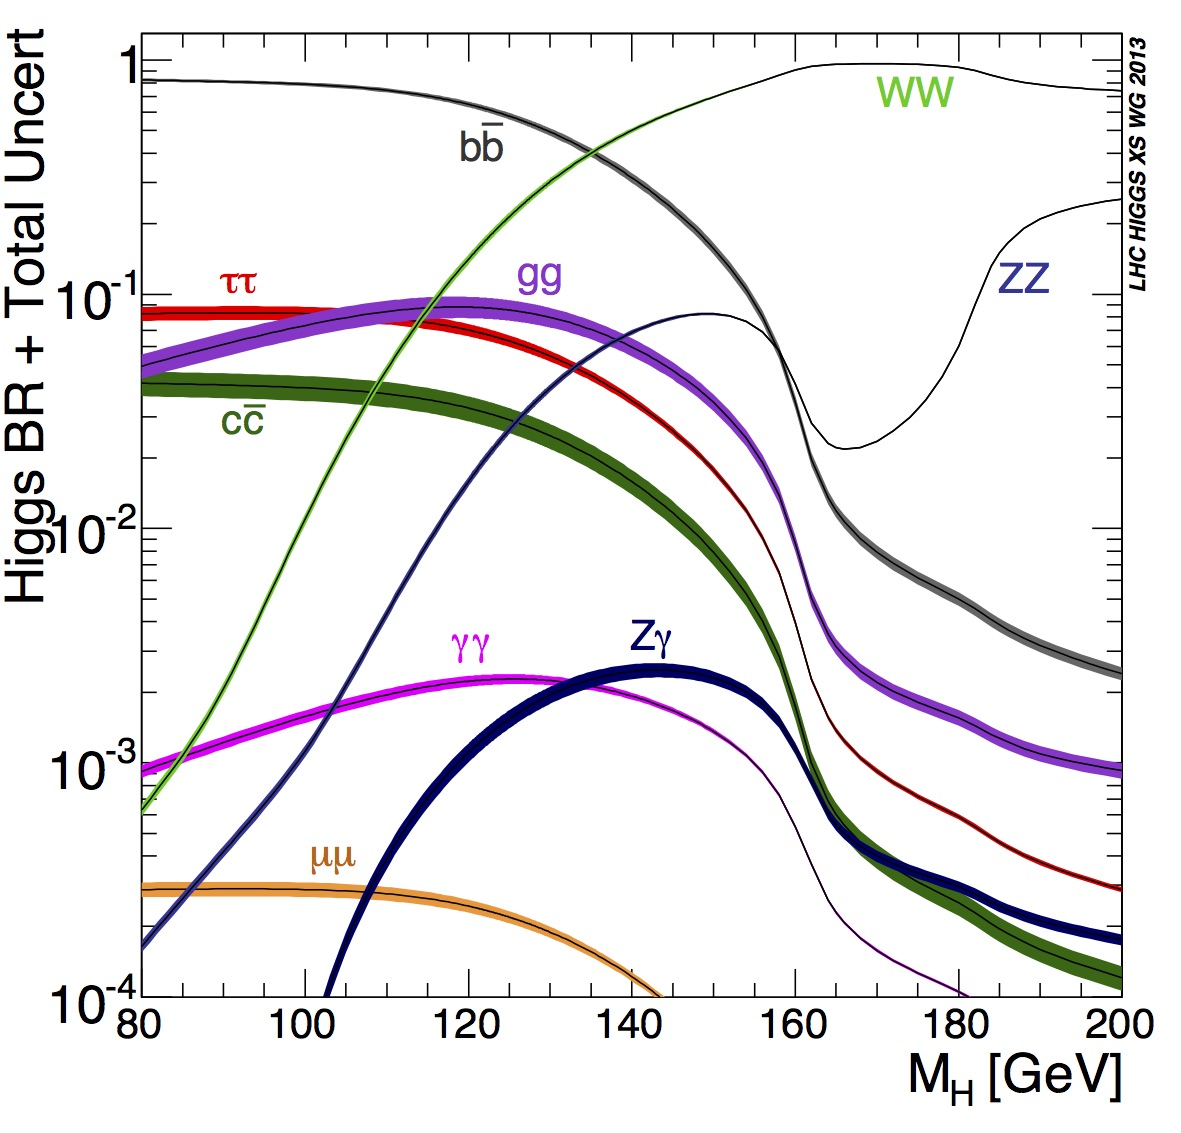
\includegraphics[width=0.45\textwidth]{figures/theory/theory_higgs_br_vs_mass.jpg}\label{fig:Higgs_BR_mass_range}
  }
\end{figure}

In the SM, the Higgs boson couples to fermions with strength proportional to their mass ($g_{Hff} = \frac{m_{f}}{v}$) and to vector bosons with a strength proportional to the square of their mass ($g_{HVV} = \frac{2m_{V}^{2}}{v}$). Figure~\ref{fig:coupling_vs_mass} shows the reduced Higgs coupling constants as a function of particle mass as measured by ATLAS\@. The results confirm the expected mass dependence of the couplings where heavier particles couple more strongly to the Higgs boson. Couplings to all vector bosons and third-generation fermions have been measured, while efforts to measure couplings to second-generation fermions are ongoing.

These coupling indicate that the Higgs boson tends to decay into the heaviest particles that are kinematically allowed. Figure~\ref{fig:Higgs_BR_mass_range} illustrates the branching ratios of the Higgs boson as a function of its mass. Since the Higgs boson coupling to vector bosons scales as $m_{V}^{2}$, decays to vector boson pairs become dominant at high Higgs boson masses, where the Higgs boson is sufficiently heavy to decay into two on-shell bosons. However, the Higgs boson we measure has mass $m_{H} = 125$ GeV, so the dominant decay channel is H $\rightarrow b\bar{b}$, since the bottom quark is the heaviest fermion accessible at this mass. Vector boson decays are suppressed because at least one of the bosons must be off-shell. 

The sub-dominant decay is $H \rightarrow WW^{*}$, followed by $H \rightarrow gg$. While $H \rightarrow gg$ has the third highest branching ratio, it has yet to be measured due to the complexities of having a two $g$ final state. Following this, the next most common decay modes are $H \rightarrow \tau^{+}\tau^{-}$, $H \rightarrow ZZ^{*}$, and $H \rightarrow \gamma\gamma$. The predicted branching ratios for a Higgs boson of mass $m_{H} = 125$ GeV is listed in Table~\ref{tab:BRs}.

\begin{table}[h]
  \centering
  \begin{tabular}{l|c}
    \hline
    Decay Channel & Branching Ratio \\
    \hline
    $H \rightarrow b\bar{b}$ & $58.2^{+1.2}_{-1.3}$~\% \\
    $H \rightarrow W^{\pm}W^{*\mp}$ & $21.4^{+1.6}_{-1.5}~\%$ \\
    $H \rightarrow gg$ & $8.2^{+5.1}_{-5.1}~\%$ \\
    $H \rightarrow \tau^{+}\tau^{-}$ & $6.3^{+1.7}_{-1.7}~\%$ \\
    $H \rightarrow ZZ^{*}$ & $2.6^{+1.6}_{-1.5}~\%$ \\
    $H \rightarrow \gamma\gamma$ & $0.23^{+2.1}_{-2.1}~\%$ \\
    \hline
  \end{tabular}
  \caption{Predicted branching ratios for the Higgs boson decay channels at $m_{H} = 125$ GeV, taken from~\cite{LHC_Higgs_handbook}.}\label{tab:BRs}
\end{table}

Among these, the $H \rightarrow WW^{*}$ channel is of particular interest for this thesis. Despite being being the sub-dominant channel, it still maintains a high branching ratio of approximately 21\% providing a substantial number of events. Furthermore, the leptonic decay $WW^{*} \rightarrow \ell\nu\ell\nu$ provides a clean experimental signature in the ATLAS detector due to the excellent lepton identification and reconstruction. This makes an ideal channel for precision studies, and forms the basis of this thesis.

To study this decay channel, we must first produce Higgs bosons which will be discussed in the following Section.

\section{Higgs Boson Production}\label{sec:theory_higgs_production}
% The Higgs boson is produced through four main production mechanisms at the LHC\@: gluon-gluon fusion (ggF), vector boson fusion (VBF), associated production with a vector boson (VH) and top fusion (ttH). The feynman diagrams for the production modes can be seen in Figure~\ref{fig:higgs_production_modes}, while Figure~\ref{fig:higgs_production_function_of_com} illustrates the production cross sections as a function of the $\sqrt{s}$ for each production mode. The dominant Higgs boson production mode at the LHC is ggF. This is followed by VBF which is an order of magnitude smaller. In the same order of magnitude is VH (Higgstrahlung), where WH has a higher cross section than ZH\@. Finally, there is ttH/bbH production which are of the same order of magnitude as ZH.

The Higgs boson is produced at the LHC primarily through four mechanisms: gluon-gluon fusion (ggF), vector boson fusion (VBF), associated production with a vector boson (VH), and associated production with top/bottom quarks (ttH/bbH). Feynman diagrams for these production modes are shown in Figure~\ref{fig:higgs_production_modes}, while Figure~\ref{fig:higgs_production_function_of_com} displays their production cross sections as functions of $\sqrt{s}$. 

\begin{figure}[pht]
  \centering
  \subfloat[Feynman diagrams for the main Higgs boson production modes. Taken from~\cite{Higgs_production_diagrams}\label{fig:higgs_production_modes}]{
    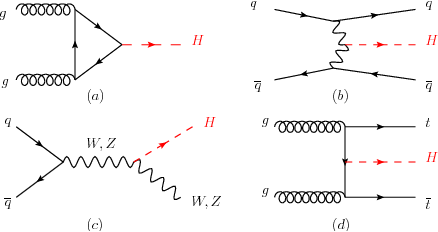
\includegraphics[width=0.55\textwidth]{figures/theory/theory_higgs_prod_feynman.png}
  }
  \hspace{0.01\textwidth}
  \subfloat[Higgs boson production cross sections as a function of $\sqrt{s}$ for the different production modes, taken from~\cite{LHC_Higgs_handbook}.\label{fig:higgs_production_function_of_com}]{
    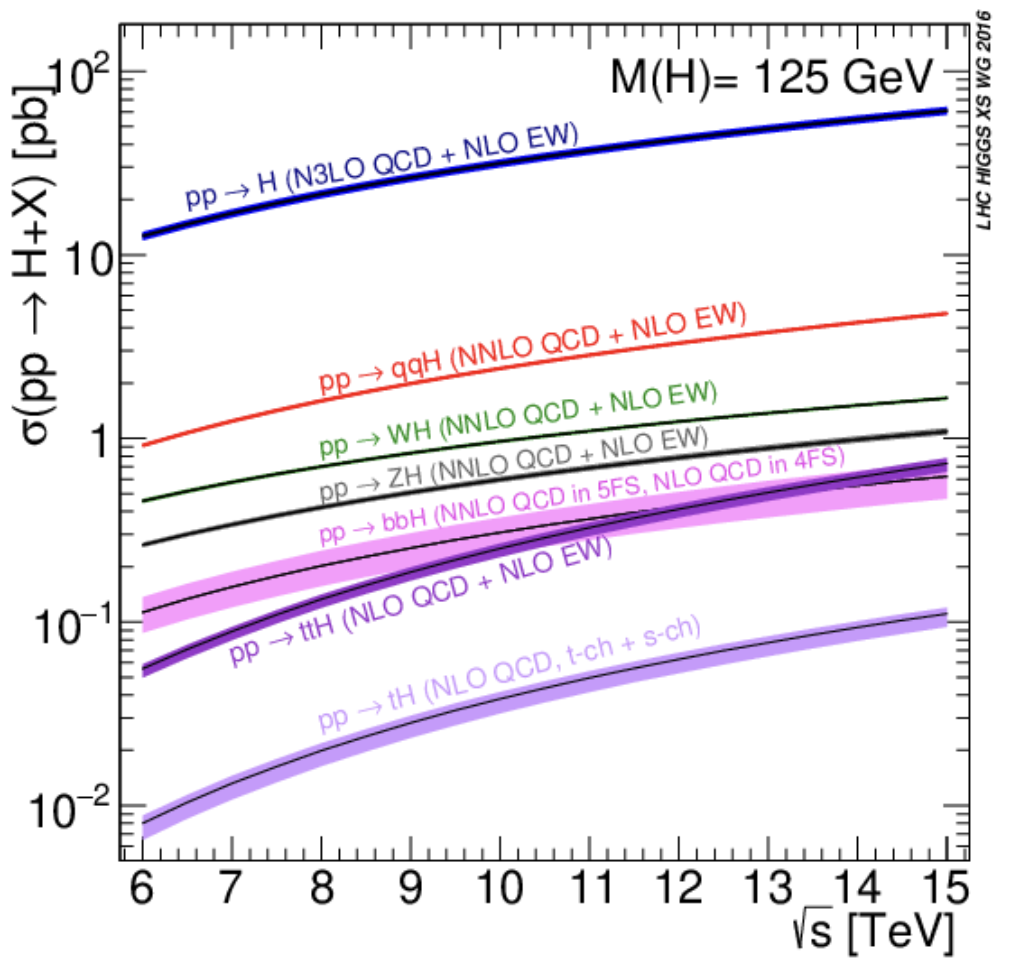
\includegraphics[width=0.35\textwidth]{figures/theory/theory_production_xs.png}
  }
  \caption{Higgs boson production mechanisms and cross sections at the LHC.}
\end{figure}

Of these, ggF ($pp \rightarrow H$) is the dominant production mechanism. Although the Higgs boson does not couple directly to gluons since they are massless, it can be produced via a loop of virtual quarks. This loop is predominantly mediated by top quarks since the Higgs boson couples to fermions with a strength proportional to their mass. The top quark is by far the heaviest known fermion, so it has the largest contribution to the ggF process.

VBF ($pp \rightarrow qqH$) follows with a cross section about an order of magnitude smaller. In this process a quark from each proton emit a $W^{\pm}$ or $Z$ boson that fuse to produce a Higgs boson. The resulting final state is characterized by two high energy forward jets. 

The VH (Higgstrahlung) process ($pp \rightarrow WH$ and $pp \rightarrow ZH$) occurs with a similar cross section to VBF\@. In these events quarks from colliding protons fuse into a vector boson, which then radiates a Higgs boson. $WH$ production occurs is more common than $ZH$ due to the the presence of two $W$ bosons and one $Z$ boson. 

Finally, ttH/bbH production ($pp \rightarrow t\bar{t}H$ and $pp \rightarrow b\bar{b}H$) are of the same order of magnitude as $ZH$. These events occur when gluons from each colliding proton decay into a $t\bar{t} \slash b\bar{b}$ pair, and then one $t \slash b$ from each proton fuse into a Higgs boson leaving a final state with two top/bottom quarks and a Higgs boson. 

For this thesis, the production mode of interest is the $VH$ production mode with a focus on the $WH$ channel. Table~\ref{tab:higgs_production_cross_sections} summarizes the production cross sections for each mechanism at $\sqrt{s} = 13$ TeV.

\begin{table}
  \centering
  \begin{tabular}{c|c}
    \hline
    Production Mode & Cross Section (pb) \\
    \hline
    ggF & $52.23^{+3.79}_{-4.69}$ \\
    VBF & $4.078^{+0.12}_{-0.12}$ \\
    $WH$ & $1.457^{+0.04}_{-0.04}$ \\
    $ZH$ & $0.9439^{+0.01}_{-0.01}$ \\
    $t\bar{t}H$ & $0.57^{+0.04}_{-0.06}$ \\
    $b\bar{b}H$ & $0.5266^{+0.11}_{-0.14}$ \\
    \hline
  \end{tabular}
  \caption{Higgs boson production cross sections at $\sqrt{s} = 13.6$ TeV for the different production modes, taken from~\cite{Higgs_production_cross_sections}.}\label{tab:higgs_production_cross_sections}
\end{table}

% \begin{figure}[pht]
%   \centering
%   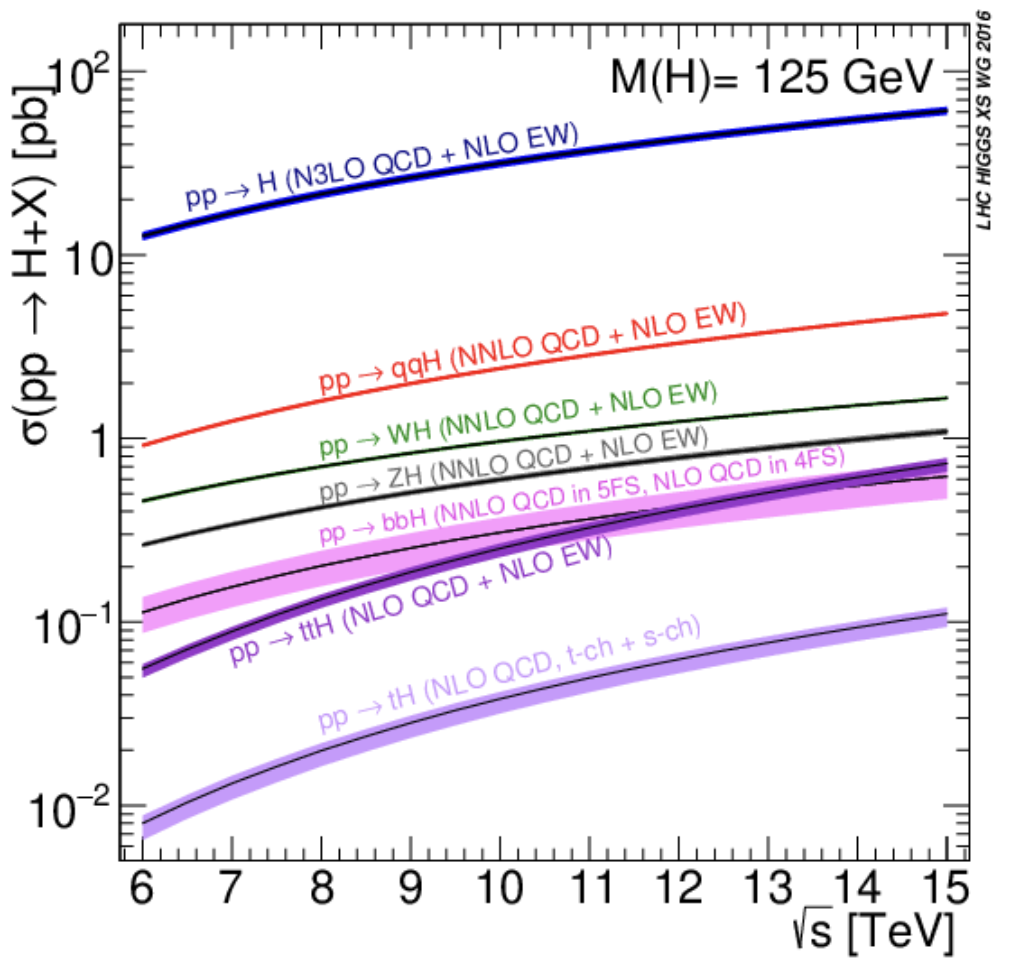
\includegraphics[width=0.6\textwidth]{figures/theory/theory_production_xs.png}
%   \caption{Higgs boson production cross sections as a function of $\sqrt{s}$ for the different production modes, taken from~\cite{LHC_Higgs_handbook}.}\label{fig:higgs_production_function_of_com}
% \end{figure}

\chapter{The ATLAS Experiment}\label{ch:atlas}
\section{The Large Hadron Collider}\label{sec:lhc}
The Large Hadron Collider (LHC) is the world's largest and most powerful particle accelerator ever built whose sole purpose is to explore the fundamental interactions of nature. The LHC is located at the European Organization for Nuclear Research (CERN) in Geneva, situated right on the border of France and Switzerland.
The LHC is 27 km in circumference and can accelerate proton beams to a center of mass energy (\com{}) of 7 TeV each, resulting in a proton-proton collision with a \com{} of 14 TeV. For heavy-ion collisions each beam can also have a maximum \com{} of 7 TeV, with each nucleon having a maximum \com{} of about 5.5 TeV. Rather than a continuous beam of protons, protons are packed together in groups consisting of many billions of protons which is referred to as a proton bunch. The proton bunches are spaced apart from other proton bunches such that collisions happen at a set interval of every 25 nanoseconds. 
Likewise for heavy ion collisions, these particles are also grouped together in bunches, but have a different bunch spacing between them, ranging from 50 ns to 100 ns~\cite{Alice_first_pb_2023}. %For proton-proton collisions, LHC was designed to operate at a nominal luminosity of $\mathcal{L} = 10^{34} \mathrm{cm}^{-2}\mathrm{s}^{-1}$ but this has since been doubled to a sustained luminosity of $\mathcal{L} = 2 \times 10^{34} \mathrm{cm}^{-2}\mathrm{s}^{-1}$, while for heavy-ion collisions the maximum sustained luminosity is $\mathcal{L} = 10^{27} \mathrm{cm}^{-2}\mathrm{s}^{-1}$~\cite{ATLAS_run3_luminosity_and_detector}.

To accelerate protons to the desirable center of mass energies, a complex accelerator chain is used to accelerate protons in phases. The start of the accelerator chain is a linear accelerator, Linac4~\cite{linac4_yellow_report}, which accelerates protons to a \com{} of 160 MeV. This detector is relatively new having only been added during the long shutdown after Run 2 data taking, and replaces the previously used Linac2, which was only able to accelerate protons to a \com{} of 50 MeV. From Linac4, the protons are passed into the Proton Synchrotron Booster (PSB), which also underwent several upgrades of its own during the Run 2 long shutdown~\cite{psb_ls2_upgrade}, and is the first synchrotron in the accelerator chain. 
The PSB accelerates protons from 160 MeV to 2 GeV, before passing the protons along to the Proton Synchrotron (PS), which accelerates protons to 26 GeV. This part of the accelerator chain is essential as the proton bunches are compressed, split, and placed into the 25 ns spacing that the LHC requires. From here, and while keeping the established structure of the bunches, the bunches are passed into the Super Proton Synchrotron (SPS) which is the last step of the accelerator chain before the LHC\@. Here, the proton bunches are accelerated up to 450 GeV and passed either clockwise, or counter-clockwise, into the LHC where they are accelerated to their desired center of mass energies. This accelerator chain is depicted in Figure~\ref{fig:lhc_accelerator_chain}.

\begin{figure}[pht]
    \centering
    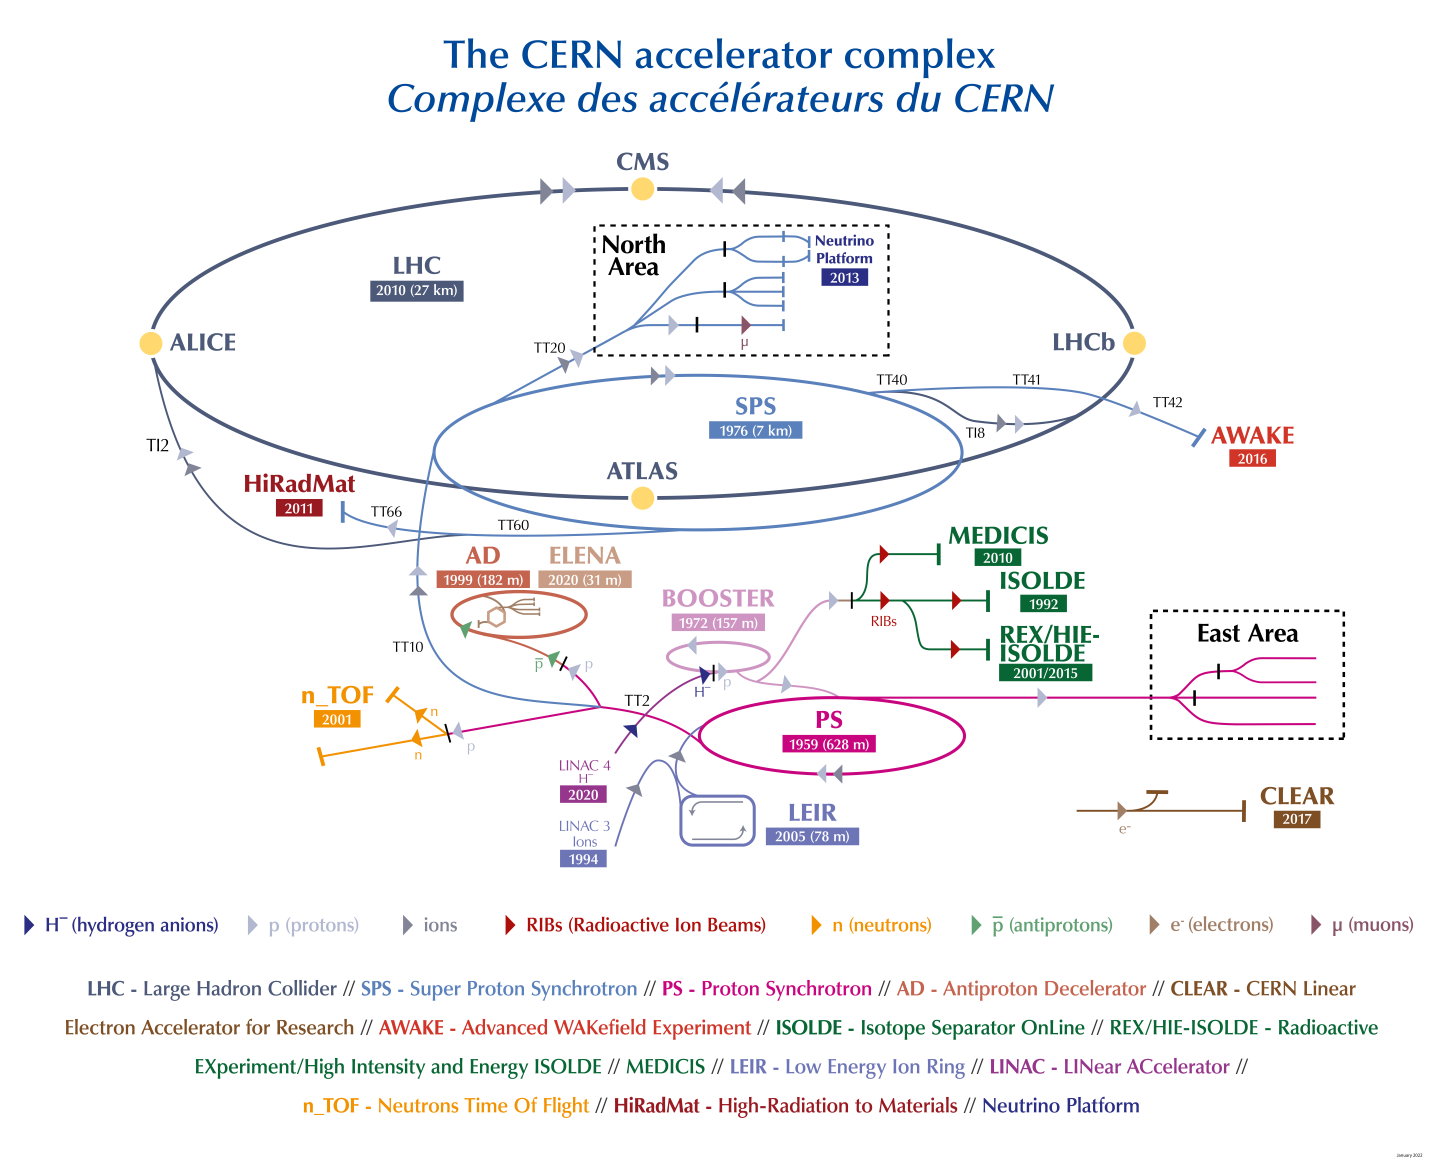
\includegraphics[width=0.7\textwidth]{figures/atlas/lhc_accelerator_chain.png}
    \caption{Shown are both the proton and heavy-ion accelerator chains. The proton accelerator chain starts from Linac4, goes to the PSB, then the PS and finally the SPS before being passed to the LHC\@. Heavy-ions follow a similar chain except their starting point is Linac3 and are then passed directly to the PS\@. Taken from~\cite{lhc_accelerator_chain_diagram}}\label{fig:lhc_accelerator_chain}
\end{figure}

At the LHC there are four main experiments. The two largest experiments, ATLAS~\cite{atlas_collaboration_paper} and CMS~\cite{cms_collaboration_paper}, are general, multi-purpose detectors designed to study a large range of topics in HEP, including precision measurements, searches for new physics, and even quark-gluon plasma from the heavy-ion collisions. There also exist two other experiments at the LHC with a more narrowed focus on their research activities. LHCb~\cite{lhcb_collaboration_paper} is a dedicated heavy-flavour physics experiment whose main goal is to search for new physics in CP violation, and rare decays of beauty and charm quarks. The ALICE~\cite{alice_collaboration_paper} experiment on the other hand is focused on heavy-ion collisions, more specifically the study of quark-gluon plasma that is produced during heavy-ion collisions. 

For Run 3, the LHC will operate at a \com{} collision energy of 13.6 TeV, and will take data from 2022--2026. The results covered in this thesis will be from the 2022 and 2023 data taking periods during Run 3.

\section{Luminosity and Pileup}\label{sec:luminosity_pileup}
% Instantaneous luminosity, $\mathcal{L} (t)$, is the rate at which colliding particles interact per unit area at a given moment in time. To determine the total number of interactions $N(t)$, the instantaneous luminosity is integrated over time and multiplied by the proton-proton interaction cross-section $\sigma_{pp}$, which characterizes the likelihood of a particular interaction:

% \begin{equation}
%     \centering
%     N(t) = \sigma_{pp} \int \mathcal{L} (t) dt
% \end{equation}

% \noindent{}The instantaneous luminosity can be defined as:

% \begin{equation}
%     \centering
%     \mathcal{L} = 2 N_1 N_2 f N_b \int \!\!\! \int \!\!\! \int \!\!\! \int_{-\infty}^{\infty} \rho_{1x}(x)\rho_{1y}(y)\rho_{1s}(s{-}s_0)\rho_{2x}(x)\rho_{2y}(y)\rho_{2s}(s{+}s_0)\, dx\, dy\, ds\, ds_0
% \end{equation}\label{eq:luminosity_long}

% \noindent{}where $N_1$ and $N_2$ are the number of particles per bunch, $f$ is the revolution frequency, $N_b$ is the number of bunches in one beam, and $\rho$ are the beam density distribution functions. Evaluating equation~\ref{eq:luminosity_long} is not always possible since all beam distributions need to be known. In many cases, it is appropriate to model these distributions as Gaussian.
% With this assumption, equation~\ref{eq:luminosity_long} simplifies to:

% \begin{equation}
%     \centering
%     \mathcal{L} = \frac{N_1 N_2 f N_b}{4\pi \sigma_x \sigma_y}
% \end{equation}

% \noindent{}The total integrated luminosity, $L$, is defined as the integral of the instantaneous luminosity over some time, $T$:
% \begin{equation}
%     \centering
%     L = \int_{0}^{T} \mathcal{L} (t) dt
% \end{equation}
% \noindent{}Thus it is seen that the total number of events is proportional to the total integrated luminosity.

% At the LHC, the nominal instantaneous luminosity is $\mathcal{L} = 10^{34} \mathrm{cm}^{-2}\mathrm{s}^{-1}$. During Runs 2 and 3, the recorded instantaneous luminosity approximately doubled the nominal value, reaching a sustained luminosity of $\mathcal{L} = 2.1 \cdot 10^{34} \mathrm{cm}^{-2}\mathrm{s}^{-1}$ for proton-proton collisions, while for heavy-ion collisions the maximum sustained luminosity recorded was $\mathcal{L} = 10^{27} \mathrm{cm}^{-2}\mathrm{s}^{-1}$~\cite{ATLAS_run3_luminosity_and_detector}. Figure~\ref{fig:atlas_luminosity_recorded} presents the total integrated luminosity delivered by the LHC and recorded by ATLAS during Run 3. Through the first three years of data taking for this run, the LHC has delivered a total of 195 $\mathrm{fb}^{-1}$ of data. Of this, ATLAS only recorded 183 $\mathrm{fb}^{-1}$ of data with only 169 $\mathrm{fb}^{-1}$ of data deemed suitable for physics analysis. These luminosity discrepancies
% arise when detector components malfunction or data-taking conditions change mid run. ATLAS maintains a record of periods with nominal conditions referred to as the ``Good Runs List'' (GRL), which defines the datasets available for further analysis.

% \begin{figure}
%     \centering
%     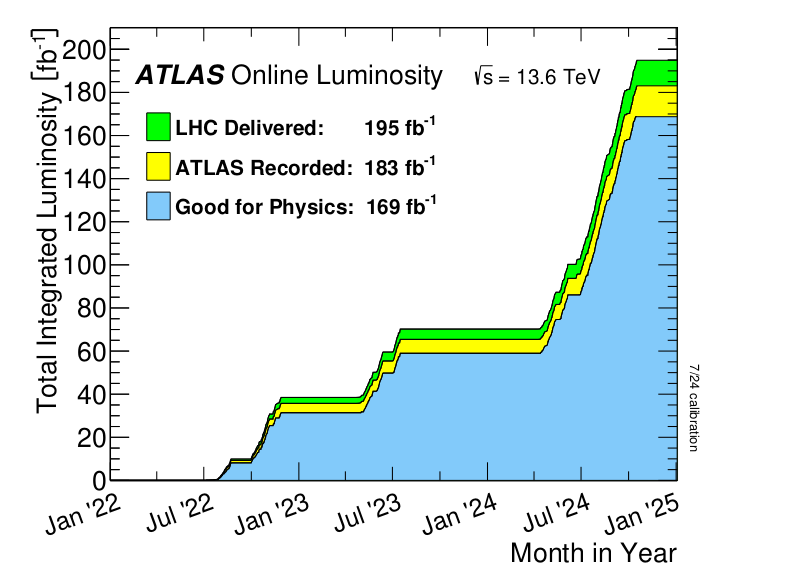
\includegraphics[width=0.8\textwidth]{figures/atlas/atlas_run3_lumi.png}
%     \caption{The total integrated luminosity delivered by the LHC and recorded by ATLAS\@. As seen in the figure, the LHC delivered and ATLAS recorded differ from one another due to non-nominal circumstances. Taken from~\cite{atlas_lumi_image}}\label{fig:atlas_luminosity_recorded}
% \end{figure}

%%% New revision
The instantaneous luminosity, $\mathcal{L}(t)$, is the rate of particle collisions per unit area at a given time. The total number of interactions, $N(t)$, is proportional to the integrated luminosity and the proton-proton- cross-section $\sigma_{pp}$
\begin{equation}
    \centering
    N(t) = \sigma_{pp} \int \mathcal{L} (t) dt
\end{equation}
The instantaneous luminosity is given by:
\begin{equation}
    \centering
    \mathcal{L} = 2 N_1 N_2 f N_b \int \!\!\! \int \!\!\! \int \!\!\! \int_{-\infty}^{\infty} \rho_{1x}(x)\rho_{1y}(y)\rho_{1s}(s{-}s_0)\rho_{2x}(x)\rho_{2y}(y)\rho_{2s}(s{+}s_0)\, dx\, dy\, ds\, ds_0
\end{equation}\label{eq:luminosity_long}
where $N_1$,$N_2$ are particles per bunch, $f$ the revolution frequency, $N_b$ number of bunches, and $\rho$ the beam density distribution functions. When the beam density distributions are modeled as Gaussians, this simplifies to
\begin{equation}
    \centering
    \mathcal{L} = \frac{N_1 N_2 f N_b}{4\pi \sigma_x \sigma_y}
\end{equation}
where $\sigma_x$ and $\sigma_y$ transverse beam widths. The integrated luminosity $L$ over time $T$ is defined as
\begin{equation}
    \centering
    L = \int_{0}^{T} \mathcal{L} (t) dt.
\end{equation}

At the LHC, the nominal instantaneous luminosity, $\mathcal{L} = 10^{34} \mathrm{cm}^{-2}\mathrm{s}^{-1}$, has been exceeded during Runs 2 and 3, and reached a sustained luminosity of $\mathcal{L} = 2.1 \cdot 10^{34} \mathrm{cm}^{-2}\mathrm{s}^{-1}$ in $pp$ collisions. For heavy-ions, peak instantaneous luminosity reached $\mathcal{L} = 10^{27} \mathrm{cm}^{-2}\mathrm{s}^{-1}$~\cite{ATLAS_run3_luminosity_and_detector}.

Figure~\ref{fig:atlas_luminosity_recorded} shows the integrated luminosity delivered to and recorded by ATLAS during Run 3\@. Of the 195 $\mathrm{fb}^{-1}$ delivered, 183 $\mathrm{fb}^{-1}$ were recorded and 169 $\mathrm{fb}^{-1}$ deemed suitable for physics analysis. The ``Good Runs List'' (GRL) defines the useable datasets and excludes periods with detector issues or unstable conditions.
\begin{figure}
    \centering
    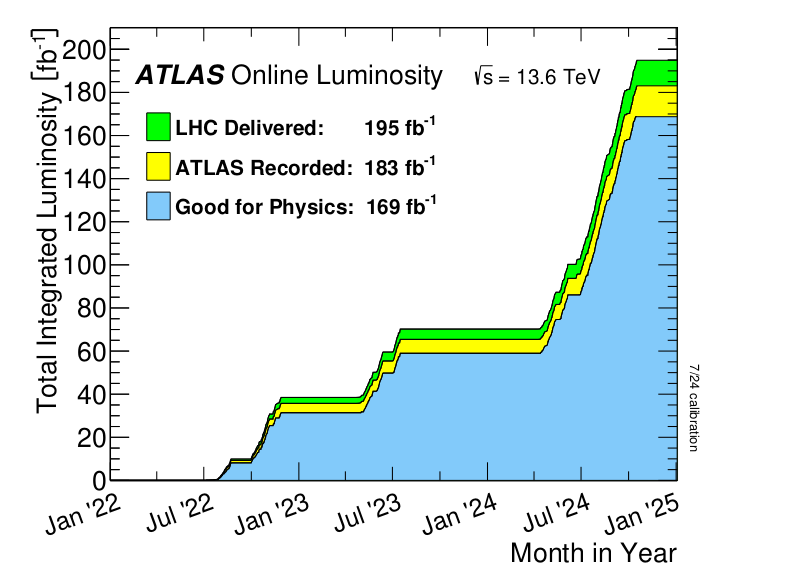
\includegraphics[width=0.8\textwidth]{figures/atlas/atlas_run3_lumi.png}
    \caption{Run 3 integrated luminosity delivered by the LHC and recorded by ATLAS\@. Differences reflect detector downtimes or suboptimal data-taking conditions. From~\cite{atlas_lumi_image}.}\label{fig:atlas_luminosity_recorded}
\end{figure}

High luminosity is required for observing the rare processes of interest at the LHC, but with it comes a key challenge: pileup. For every bunch crossing, there is one hard scattering process that produces the physics of interest, and many softer interactions that occur simultaneously and are called pileup. Pileup is quantified by the average number of interactions per bunch crossing, $\langle \mu \rangle$, which has increased throughout Run 3. In 2022 $\langle \mu \rangle = 43$, in 2023 $\langle \mu \rangle = 51$, and in 2024 $\langle \mu \rangle = 58$~\cite{atlas_pileup_image}. Mitigation strategies exist and include exploiting the granularity of the Inner Detector and various software-based techniques. Figure~\ref{fig:atlas_run3_pileup} shows the pileup distributions during the first three years of Run 3.

\begin{figure}
    \centering
    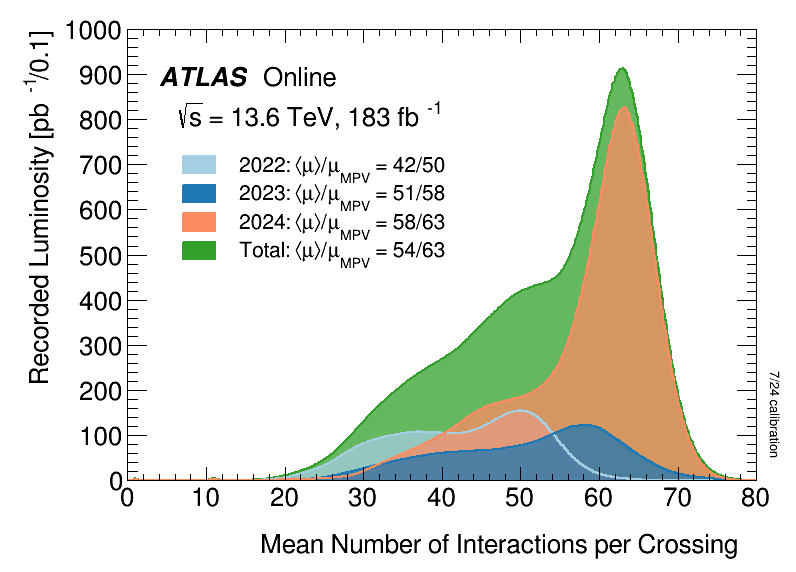
\includegraphics[width=0.8\textwidth]{figures/atlas/atlas_run3_pileup.png}
    \caption{The luminosity-weighted distribution for the mean number of interactions per bunch crossing for 2022--2024 pp collision data. Taken from~\cite{atlas_pileup_image}}\label{fig:atlas_run3_pileup}
\end{figure}

% \section{Pileup}\label{sec:pileup}
% % Proton bunches at the LHC contain approximately $10^{11}$ protons which is necessary to achieve the high luminosities discussed in the prior section. Unfortunately, due to the large number of protons in a proton bunch multiple interactions happen per bunch crossing. During the crossing, there is one primary inelastic hard scattering event, which produces the physics of interest. Additionally, there are many soft scattering collisions, referred to as pileup, which obscure the collision of interest.

% As luminosity increases, so does pileup, presenting a trade off between achieving high luminosity and high pileup or low luminosity and low pileup. The physics processes of interest at the LHC are rare, and thus require high luminosity, so efforts are focused on mitigating the resulting pileup. One strategy involves leveraging the granularity of the Inner Detector as described in Section~\ref{sec:atlas_id}, which can help distinguish between the primary interaction and the softer interactions. Additionally, software based techniques used during event reconstruction can help suppress pileup effects, and are further discussed in Chapter~\ref{ch:reco}.
% Pileup is quantified by the average number of interactions per bunch crossing, $\langle \mu \rangle$, which is determined from the luminosity block (lb), which is defined as a short interval over which the instantaneous luminosity is approximately constant. The average value of $\langle \mu \rangle$ was 43 in 2022, 51 in 2023, and 58 in 2024~\cite{atlas_pileup_image}. Figure~\ref{fig:atlas_run3_pileup} shows the pileup distributions during the first three years of Run 3.

% \begin{figure}
%     \centering
%     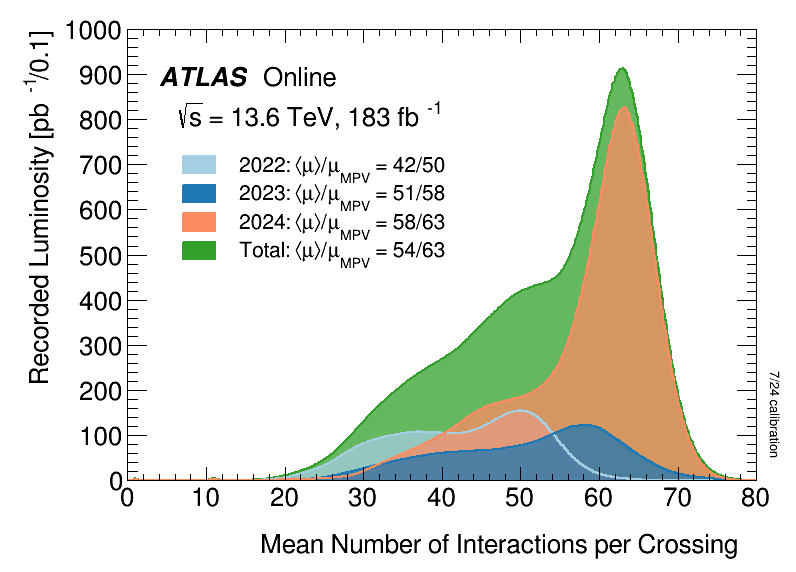
\includegraphics[width=0.8\textwidth]{figures/atlas/atlas_run3_pileup.png}
%     \caption{Shown is the luminosity-weighted distribution for the mean number of interactions per bunch crossing for 2022--2024 pp collision data. Taken from~\cite{atlas_pileup_image}}\label{fig:atlas_run3_pileup}
% \end{figure}

High luminosity is required for observing the rare processes of interest at the LHC, but with it comes a key challenge: pileup. For every bunch crossing, there is one hard scattering process that produces the physics of interest, and many softer interactions that occur simultaneously which complicate event reconstruction which are referred to as pileup.

Pileup is characterized by the average number of interactions per bunch crossing, $\langle \mu \rangle$, which has increased throughout Run 3. In 2022, $\langle \mu \rangle$ was 43, in 2023 it was 51, and in 2024 it was 58~\cite{atlas_pileup_image}. Mitigiation strategies exist and include exploiting the granularity of the Inner Detector and various software-based techniques. Figure~\ref{fig:atlas_run3_pileup} shows the pileup distributions during the first three years of Run 3.

\begin{figure}
    \centering
    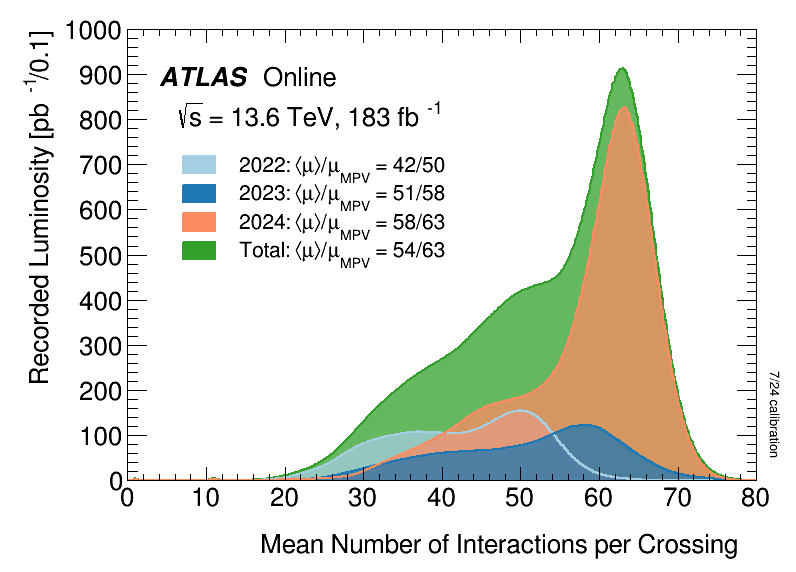
\includegraphics[width=0.8\textwidth]{figures/atlas/atlas_run3_pileup.png}
    \caption{The luminosity-weighted distribution for the mean number of interactions per bunch crossing for 2022--2024 pp collision data. Taken from~\cite{atlas_pileup_image}}\label{fig:atlas_run3_pileup}
\end{figure}

\section{The HL-LHC}\label{sec:hl_lhc}
Following the completion of Run 3, the LHC will enter its third long shutdown (LS3). During LS3 the LHC and its major experiments will undergo massive upgrades in preparation for Run 4. For example, the LHC will upgrade numerous technologies such as the superconducting magnets, the radio frequency cavities, and the beam collimation systems~\cite{lhc_upgrade_run4}. The HL-LHC aims to deliver significantly more luminosity than it currently does in Run 3, expecting to sustain a luminosity of 5 to 7.5 times larger than the nominal LHC values. Along with the increased luminosity,
the energy of each proton beam is expected to have a \com{} of 7 TeV, producing proton-proton collisions with a \com{} of 14 TeV. 

Additionally, ATLAS will also be performing upgrades to their detector systems~\cite{atlas_detector_upgrade_run4}, data acquisition and trigger systems~\cite{atlas_detector_upgrade_run4}, as well as their computing and software infrastructure~\cite{CERN-LHCC-2022-005}. These upgrades, particularly those in software and computing, are critical to meet the demands of the HL-LHC era which is expected to bring higher event rates with over double the number of interactions per bunch crossing in comparison to Run 3, and over 10x more data collected than Run 1, 2 and 3 combined.
Figure~\ref{fig:atlas_cpu_usage} shows the expected CPU consumption required per year for ATLAS depending on two different R\&D scenarios. Aggressive R\&D assumes significant improvements in areas such as track reconstruction (e.g.\ a 20\% reduction in reconstruction time), a reduced amount full simulation events (reduced by 10\% to 30\%) and an increase in dedicated software and computing efforts, via new personnel or current personnel committing more time to development. In contrast, the conservative scenario assumes that current staff levels remain constant, no additional person-power and no loss of key experts.
Even with a sustained budget increase of 10\% for software and computing, neither scenario is expected to fully meet the CPU demands of the HL-LHC\@. However, if funding levels are increased by 20\% annually, the aggressive R\&D is projected to fulfill the required CPU capacity.

\begin{figure}[pht]
    \centering
    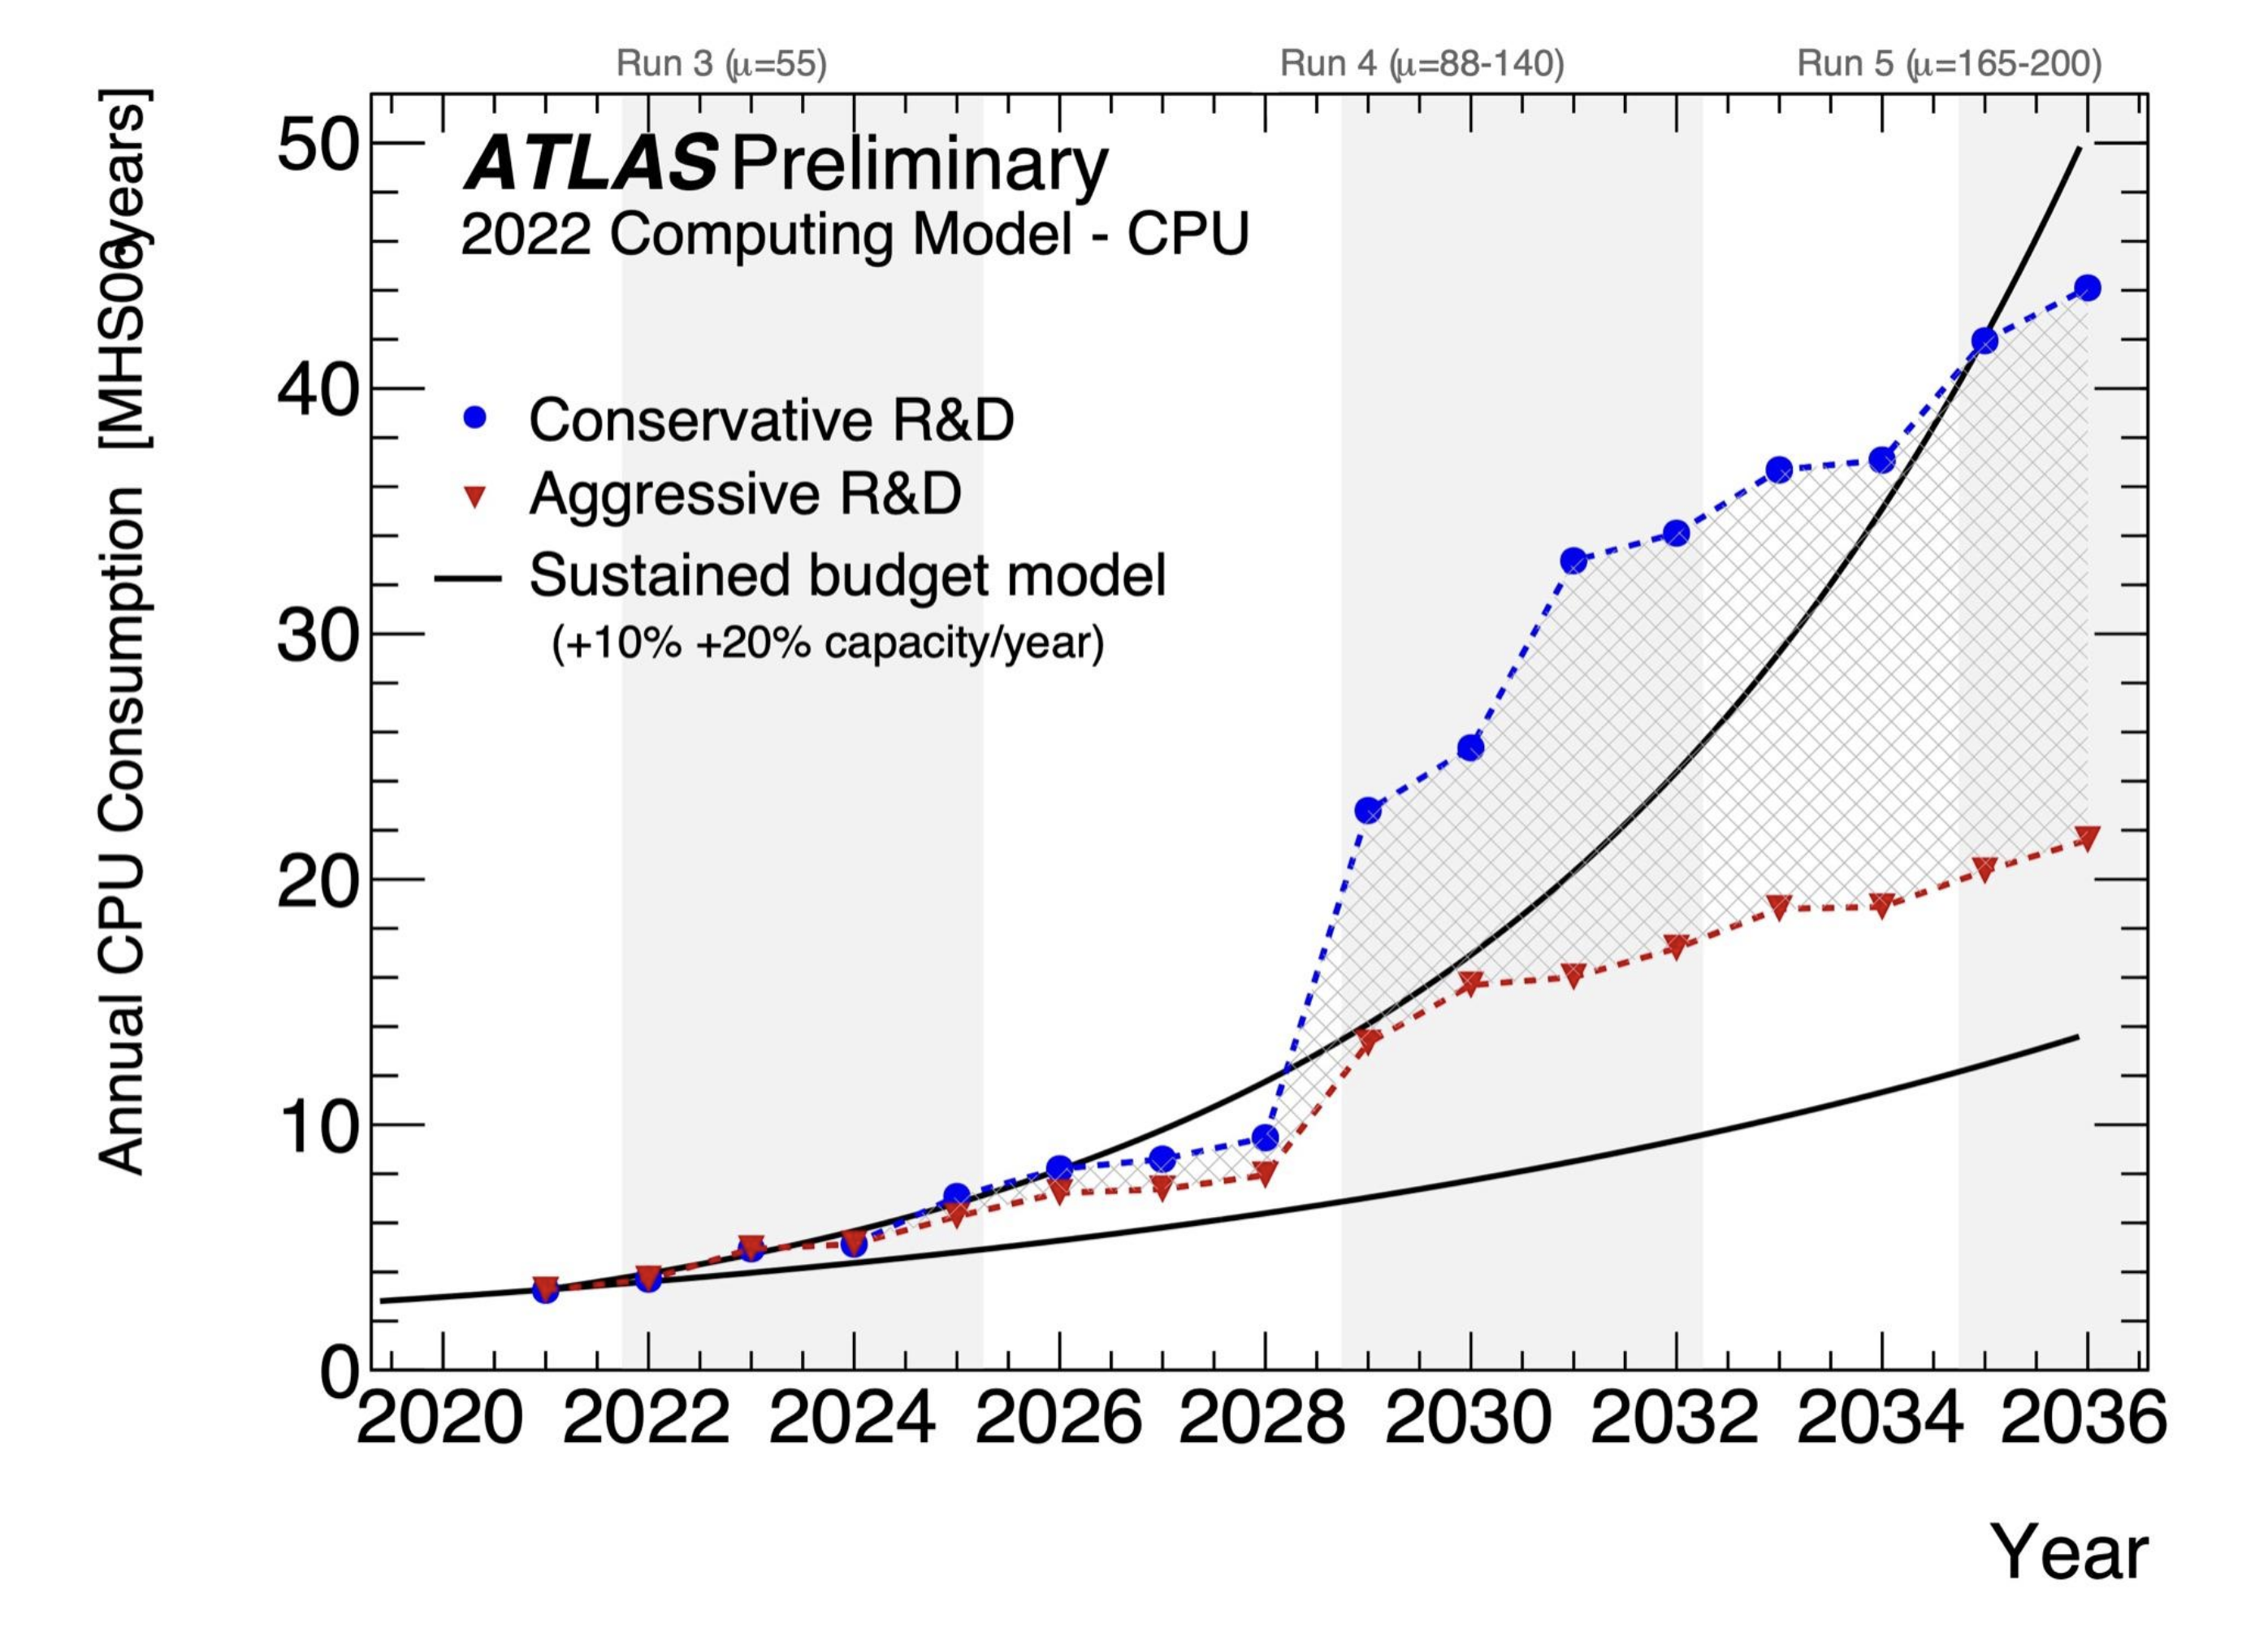
\includegraphics[width=0.9\textwidth]{figures/atlas/atlas_cpu_usage.png}
    \caption{The expected annual CPU usage for ATLAS during HL-LHC\@. The blue line shows the conservative R\&D scenario, which doesn't meet the anticipated demand for a 10\% or 20\% budget increase. The red line depicts the aggressive R\&D scenario and shows that with a 20\% budget increase yearly, the CPU demand can be fulfilled. Taken from~\cite{CERN-LHCC-2022-005}
    }\label{fig:atlas_cpu_usage}
\end{figure}

In this thesis, particular focus will be given to the software infrastructure developed for HL-LHC muon track reconstruction, which will be discussed in more detail in Chapter~\ref{ch:reco}.


\section{The ATLAS Detector}\label{sec:atlas_detector}
The ATLAS experiment, in its current form, was first proposed in 1994~\cite{atlas_technical_proposal}, with official funding from CERN member states following in 1995. Construction began in 2003 and was completed in 2008. ATLAS is the largest of the LHC's detectors, measuring 46 meters in length, 25 meters in diameter, and weighing over 7,000 tonnes. It has a symmetric, cylindrical geometry designed to provide nearly full solid-angle coverage about the collision point. The detector is made up of several subsystems arranged as concentric cylindrical layers aligned with the beam pipe. These are further divided into three main regions: the central barrel and two endcaps at either end.

The innermost component of ATLAS is the Inner Detector (ID), which is responsible for tracking charged particles and reconstructing the primary vertex (PV). The ID consists of three technologies: the high-granularity silicon pixel detector situated closest to the interaction point, followed by the Semiconductor Tracker (SCT), and finally the Transition Radiation Tracker (TRT). Surrounding the ID is the calorimeter system, split into the electromagnetic calorimeter, which measures particles like electrons and photons, and the hadronic calorimeter, which captures energy from hadrons such as pions and neutrons. The outermost subsystem is the muon spectrometer, which identifies and measures the momentum of muons, the only charged particles capable of penetrating the entire detector.
The ID is explained in more detail in Section~\ref{sec:atlas_id}, the calorimeter system in Section~\ref{sec:atlas_calorimeter}, and the muon spectrometer in Section~\ref{sec:atlas_muon}. The entire ATLAS detector can be seen in Figure~\ref{fig:atlas_detector}.

\begin{figure}[pht]
    \centering
    \includegraphics[width=0.9\textwidth]{figures/atlas/atlas_detector.png}
    \caption{Shown is ATLAS with its Run3 detector configuration. The inner detectors are seen in the middle of the figure, followed by the calorimeters, and finally by the muon spectrometer. Taken from~\cite{atlas_figure}}\label{fig:atlas_detector}
\end{figure}

\subsection{The ATLAS Coordinate System}\label{sec:atlas_coordinate_system}
% ATLAS uses a right-handed coordinate system, with origin located at the interaction point (IP). The $z$-axis runs along the beam line, the positive $x$-axis points towards the center of the LHC, and the positive $y$-axis points upwards. The positive $z$-axis is referred to as `side A', with the negative side referred to as `side C'.  More conveniently, polar coordinates are used in the transverse plane to take advantage of the cylindrical symmetry of the detector.
% The standard notation for polar coordinates is used:

% \begin{equation}
%     r = \sqrt{x^2 + y^2}
% \end{equation}\label{eq:transverse_radius}

% \begin{equation}
%     \varphi = \arctan\left(\frac{y}{x}\right)
% \end{equation}\label{eq:transverse_phi}

% \noindent{}The angle between the beam axis and the particles trajectory is defined as the polar angle $\theta$:

% \begin{equation}
%     \theta = \arctan\left(\frac{r}{z}\right)
% \end{equation}\label{eq:polar_angle}

% \noindent{}In particle physics it is more common to use the pseudorapidity $\eta$, which represents the angle of a particle with respect to the beam axis, and is defined as:

% \begin{equation}
%     \eta = -\ln\left(\tan\left(\frac{\theta}{2}\right)\right)
% \end{equation}\label{eq:pseudorapidity}

% \noindent{}Thus the commonly used, and preferred, coordinate system is represented by (r, $\varphi$, $\eta$) where the distance between two objects can be defined by:

% \begin{equation}
%     \Delta R = \sqrt{{(\Delta \eta)}^2 + {(\Delta \varphi)}^2}
% \end{equation}\label{eq:delta_R}

% \noindent{}An illustration of the coordinate system can be seen in Figure~\ref{fig:atlas_coordinate_system}.

% \begin{figure}
%     \centering
%     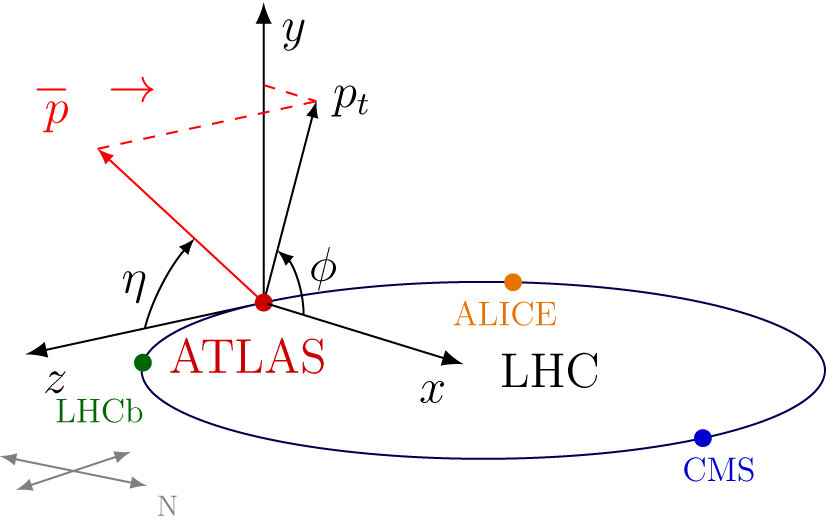
\includegraphics[width=0.9\textwidth]{figures/atlas/atlas_coordinate_system.jpg}
%     \caption{Depicted is the traditional (x,y,z) coordinate system overlaid with the cylindrical coordinate system used by physicists. Taken from~\cite{atlas_coordinate_system}}\label{fig:atlas_coordinate_system}
% \end{figure}

%%%%%%%%%%%%%%% revision
ATLAS uses a right-handed coordinate system with the origin at the interaction point (IP). The $z$-axis follows the beam line, positive $x$ points towards the LHC center, and positive $y$ upwards. The positive $z$ direction is referred to as `side A', and the negative `side C'.  Due to the detector's cylindrical symmetry, transverse polar coordinates are used where $r = \sqrt{x^2 + y^2}$ and $\varphi = \arctan\left(\frac{y}{x}\right)$. 
The angle between the beam axis and the particle's trajectory is defined as the polar angle $\theta = \arctan\left(\frac{r}{z}\right)$. In particle physics, pseudorapidity $\eta$ is preferred and is related to the polar angle via $\eta = -\ln\left(\tan\left(\frac{\theta}{2}\right)\right)$. The commonly used coordinate system is represented by (r, $\varphi$, $\eta$), where the distance between two objects can be defined as $\Delta R = \sqrt{{(\Delta \eta)}^2 + {(\Delta \varphi)}^2}$. An illustration of the coordinate system can be seen in Figure~\ref{fig:atlas_coordinate_system}.
\begin{figure}
    \centering
    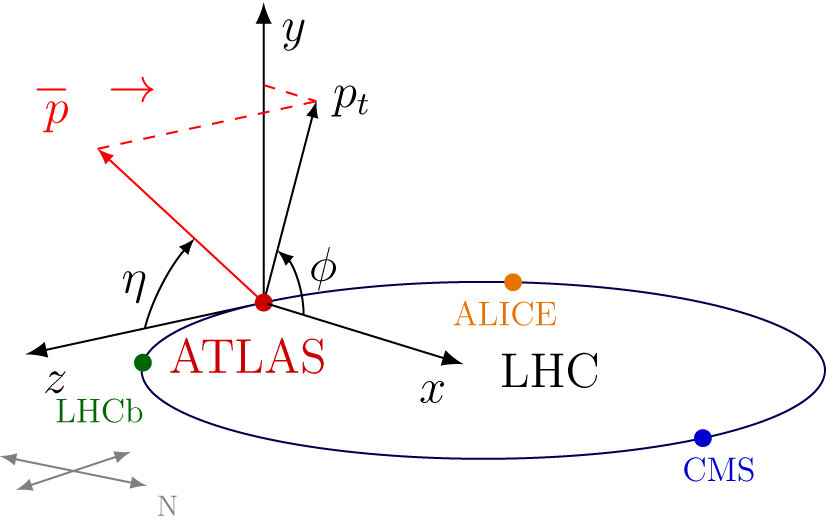
\includegraphics[width=0.9\textwidth]{figures/atlas/atlas_coordinate_system.jpg}
    \caption{Depicted is the traditional (x,y,z) coordinate system overlaid with the cylindrical coordinate system used by physicists. Taken from~\cite{atlas_coordinate_system}}\label{fig:atlas_coordinate_system}
\end{figure}

\subsection{The ATLAS Magnet System}\label{sec:atlas_magnet}
% A crucial component of any particle physics experiment is the magnet system, which enables the bending of charged particle trajectories allowing their momentum and charge to be measured. In ATLAS, this is achieved through a combination of two types of superconducting magnet systems, solenoidal and toroidal.

% The main elements of the ATLAS magnet system include the central solenoid~\cite{atlas_central_solenoid}, the barrel toroid~\cite{atlas_barrel_toroid}, and the end-cap toroids~\cite{atlas_endcap_toroid}. An illustration of the magnetic system can be seen in Figure~\ref{fig:atlas_magnetic_field_map}. The central solenoid surrounds the ID, measuring 5.8 meters in length and 2.56 meters in diameter, and provides a uniform magnetic field of 2~T to the ID region.

% \begin{figure}
%     \centering
%     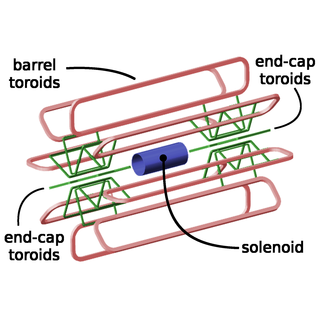
\includegraphics[width=0.55\textwidth]{figures/atlas/atlas_magnetic_system_illustration.png}
%     \caption{A rough schematic of the ATLAS magnetic system. In the center is the superconducting solenoid for the ID, followed by the MS magnet system that consists of eight large barrel toroids and two large end-cap toroids. Taken from~\cite{atlas_magnetic_system_illustration}}\label{fig:atlas_magnet_system}
% \end{figure}

% The barrel and end-cap toroids, in contrast, generate a non-uniform magnetic field that can reach up to 3.5~T, which is essential for accurately measuring the momentum of muons. The barrel toroid is composed of eight coils and is the largest toroidal magnet ever constructed, with a total length of 25.3 meters. On both sides of the barrel are the two end-cap toroids, each with a diameter of 10.7 meters.

% During operation, all of these magnets are cooled to about 4.5 K, in order to provide the necessary strong magnetic fields that are required for the experiment.
% The magnetic field configuration in the transverse plane and longitudinal plane can be seen in Figure~\ref{fig:atlas_magnetic_field_map}.

% \begin{figure}[pht]
%     \centering
%     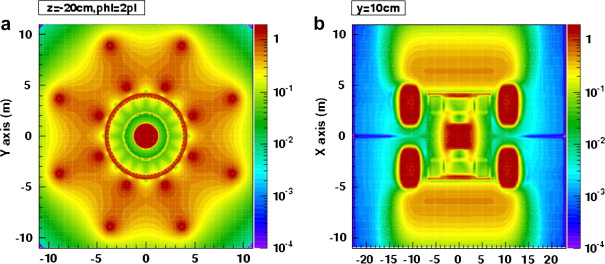
\includegraphics[width=0.8\textwidth]{figures/atlas/atlas_magnetic_field.jpg}
%     \caption{A heatmap of the magnetic field strength in different cross section views of ATLAS\@. On the left, this shows the magnetic field in the transverse plane, hence no end-cap toroidal field. The figure on the right shows the magnetic field strength in the longitudinal plane. Taken from~\cite{atlas_magnetic_field_map}}\label{fig:atlas_magnetic_field_map}
% \end{figure}

%%%%%%%%%%%% %%% revision
A crucial component of any particle physics detector is its magnet system, which bends charged particle trajectories to determine their momentum and charge. ATLAS uses two types of superconducting magnet systems, solenoidal and toroidal.

The central solenoid~\cite{atlas_central_solenoid} surrounds the ID and measures 5.8 m in length and 2.56 m in diameter and generates a uniform 2 T magnetic field. The barrel and end-cap toroids~\cite{atlas_barrel_toroid, atlas_endcap_toroid} create a magnetic field for the MS that is highly inhomogeneous and can reach up to 3.5 T. The barrel toroids are the largest ones ever constructed and consists of 8 coils spanning 25.3 m, while each end-cap has a 10.7 m diameter.

All magnets operate at 4.5 K to provide the strong magnetic fields that are required. The overall magnetic system can be seen in Figure~\ref{fig:atlas_magnet_system}, while the magnetic field configuration in the transverse and longitudinal planes is shown in Figure~\ref{fig:atlas_magnetic_field_map}.
\begin{figure}
    \centering
    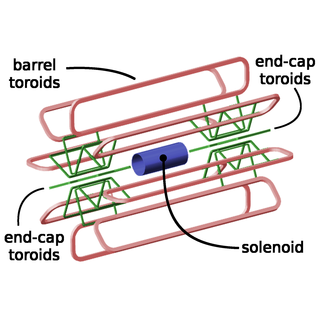
\includegraphics[width=0.55\textwidth]{figures/atlas/atlas_magnetic_system_illustration.png}
    \caption{A rough schematic of the ATLAS magnetic system. In the center is the superconducting solenoid for the ID, followed by the MS magnet system that consists of eight large barrel toroids and two large end-cap toroids. Taken from~\cite{atlas_magnetic_system_illustration}}\label{fig:atlas_magnet_system}
\end{figure}
\begin{figure}[pht]
    \centering
    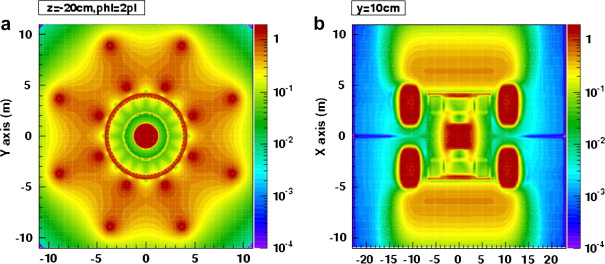
\includegraphics[width=0.8\textwidth]{figures/atlas/atlas_magnetic_field.jpg}         
    \caption{A heatmap of the magnetic field strength in different cross section views of ATLAS\@. On the left, this shows the magnetic field in the transverse plane, hence no end-cap toroidal field. The figure on the right shows the magnetic field strength in the longitudinal plane. Taken from~\cite{atlas_magnetic_field_map}}\label{fig:atlas_magnetic_field_map}
\end{figure}


\subsection{Inner Detector}\label{sec:atlas_id}
The ID is the innermost part of the ATLAS detector and measures the direction, momentum, and charge of charged particles produced in the proton-proton collision. When charged particles travel away from the interaction point (IP), they deposit energy in the sub-detectors of the ID, which are referred to as hits. These hits are then used to reconstruct the trajectory, referred to as tracks, of the particle via track reconstruction. This allows the charge and momentum of particles to be determined. Due to a large influx of particles during the proton-proton collision, the ID is designed to make high-precision measurements because of its high granularity. 

As mentioned in Section~\ref{sec:atlas_magnet}, the ID is surrounded by the superconducting solenoid, which provides a uniform 2~T magnetic field inside of the ID\@. This allows particles to curve and give the required information needed for track reconstruction. The ID only reconstructs charged particles whose momentum in the transverse plane (\pt) is above 500 MeV and within the pseudorapidity range of $|\eta| < 2.5$. The ID can be seen in Figure~\ref{fig:atlas_id}.

\begin{figure}
    \centering
    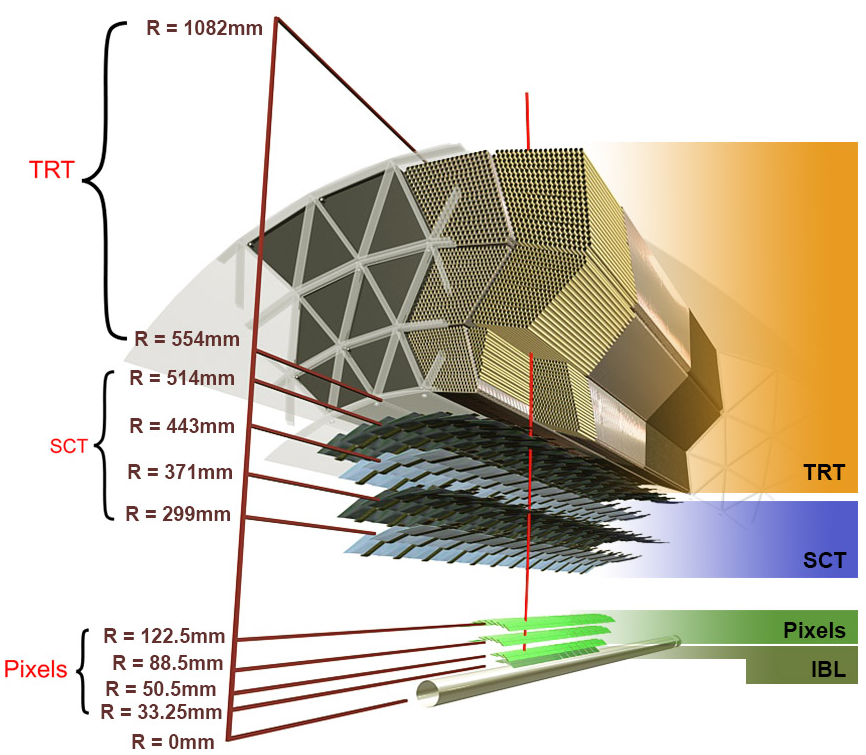
\includegraphics[width=0.8\textwidth]{figures/atlas/atlas_ID.png}
    \caption{A cross sectional view of the barrel region of the ID is shown. Depicted is a particle originating from the IP traversing through the four layers of the pixel detector, through the SCT and finally through many TRT straws. Taken from~\cite{atlas_inner_detector_image}}\label{fig:atlas_id}
\end{figure}

\begin{figure}
    \centering
    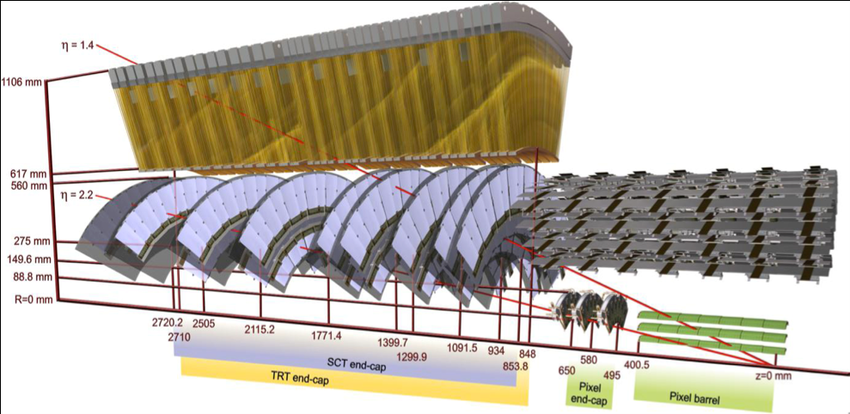
\includegraphics[width=0.8\textwidth]{figures/atlas/atlas_ID_endcap.png}
    \caption{A schematic of the ID end-cap detectors with several red lines drawn at different $\eta$ values, demonstrating a particle traversing through the detector. Additionally, this schematic shows all of the different detector technologies in the end-cap region. Taken from~\cite{atlas_inner_detector_endcap_image}}\label{fig:atlas_id_endcap}
\end{figure}

\subsubsection{Pixel Detector}\label{sec:atlas_pixel}
As mentioned, the ID is composed of three different sub-detectors. The innermost sub-detector is the pixel detector~\cite{pixel_detector_2008}~\cite{pixel_detector_ibl}. The pixel detector consists of four layers in the barrel region, and three forward disks on either side of the IP\@. When a charged particle passes through the pixel detector, it ionizes the silicon, creating electron-hole pairs along the path it takes. A strong bias voltage is applied across the sensor, so when the electron-hole pairs are created, they are pulled in opposite directions and drift towards electrodes, producing an electric signal. 
The original ATLAS pixel detector features 80 million, small rectangular pixels, with dimensions of 50 microns in the $\varphi$ direction and 400 microns in the $z$ or $r$ direction depending on barrel or end-cap region. These pixels are grouped into sensor modules with each module containing 46,080 pixels. Each module is mounted onto a mechanical and cooling support structure called a stave. Staves in the barrel region contain 13 modules, while the end-cap equivalent to staves, sectors, each contain 6 modules.

The Insertable B-Layer (IBL) is the innermost sub-detector of the ATLAS Pixel Detector system and was added between Run 1 and Run 2 to enhance tracking performance under the higher luminosity conditions expected in later runs. Positioned just 3.3 cm from the beam pipe, the IBL incorporates two different sensor technologies, planar sensors and 3D sensors, to maintain or improve the robustness and performance of ATLAS tracking given the higher luminosities expected during Run 2 and beyond. Unlike the original pixel detector, the IBL has different sized pixels, allowing for more granular measurements. Each pixel in the IBL is 50 microns in the $\varphi$ direction and 250 microns in the $z$ or $r$ direction, resulting in a 60\% smaller pixel. The IBL consists of 14 staves, with each stave containing 32 modules and each module containing 26,880 pixels. This results in an additional 12 million readout channels for the ID\@.

Following the IBL are the three original barrel pixel layers, often referred to as B-Layer 0, B-Layer 1, and B-Layer 2, located at 5.05 cm, 8.85 cm, and 12.25 cm from the beam pipe, respectively. These layers contain 22, 38 and 52 staves respectively resulting in 13.2, 22.8, and 31.2 million readout channels for a combined 67 million readout channels.

In addition to the barrel layers, the Pixel Detector includes three end-cap disks on each side of the interaction point. These disks are positioned at approximately 40.05 cm, 58.0 cm, and 65.0 cm from the IP, with each disk containing 8 sectors, resulting in approximately 13.3 million more readout channels.
\subsubsection{Semiconductor Tracker}\label{sec:atlas_sct}
Surrounding the pixel detector is the Semiconductor Tracker (SCT)~\cite{atlas_sct}, whose purpose, like the pixel detector, is to detect charged particles as they propagate away from the IP\@. Hits in this sub-detector are detected via the same mechanisms as the pixel detector\@. Different from the pixel detector, however, is that this sub-detector consists of 4088 modules of silicon-strip detectors. Each module consists of 770 strips, with the modules arranged in four concentric barrels around the pixel-detector. Additionally, there are two end-cap parts of the SCT each consisting of nine disks. The barrel layer of the SCT contains 528 silicon-strip detectors, and the end-cap regions contain 494 strip-detectors each. In the barrel region, modules are glued back to back to each other resulting in a maximum of 8 hits being registered in the barrel region, while the end-caps contain 9 single-sided modules, resulting in a maximum of 9 hits. 
\subsubsection{Transition Radiation Tracker}\label{sec:atlas_trt}
The final layer of the ID is a sub-detector called the Transition Radiation Tracker (TRT)~\cite{atlas_trt} which utilizes gas-filled drift tubes for detecting charged particles, unlike the other sub-detectors. The TRT is composed of 300,000 thin-walled drift tubes, often referred to as straws, each filled with a gas mixture of xenon (70\%), $\mathrm{CO}_2$ (27\%) and $\mathrm{O}_2$ (3\%). This choice of gas is no coincidence with xenon being used due to its good X-ray absorption, while the two other gases help increase electron drift velocity, and suppress photon quenching. 

Each straw is 4 mm in diameter with a gold-plated tungsten wire located in the center of the tube that is kept grounded. The exterior of the straw is kept at high voltage with negative polarity creating an electric field between the walls and the wire. When a charged particle passes through a straw, the gas inside the straw ionizes, creating free electrons. The free electrons drift towards the wire because of the voltage differential and produce a signal that is amplified and read out via both ends of the tube.

In addition, the TRT is designed to detect transition radiation photons. When a charged particle traverses the boundary between materials with different dielectric constants, in the case of the TRT these are polymer fibres and foils, soft X-ray photons are produced. These photons are detected in the straws by being absorbed by the xenon atoms which ionize, creating a free electron that drifts to the central wire. Transition radiation is a function of $\gamma$ and is defined as $\gamma = \frac{E}{m}$. Therefore, a light particle, such as an electron, emits a lot more photons than a heavier particle, such as a pion with the same energy. When an excess of energy is deposited in a straw, beyond what is expected for the usual ionizing particles, it is a strong indication that the particle is an electron.
A cross sectional view of the TRT with a particle passing through some straw tubes can be seen in Figure~\ref{fig:atlas_trt_straw_hits}.

\begin{figure}
    \centering
    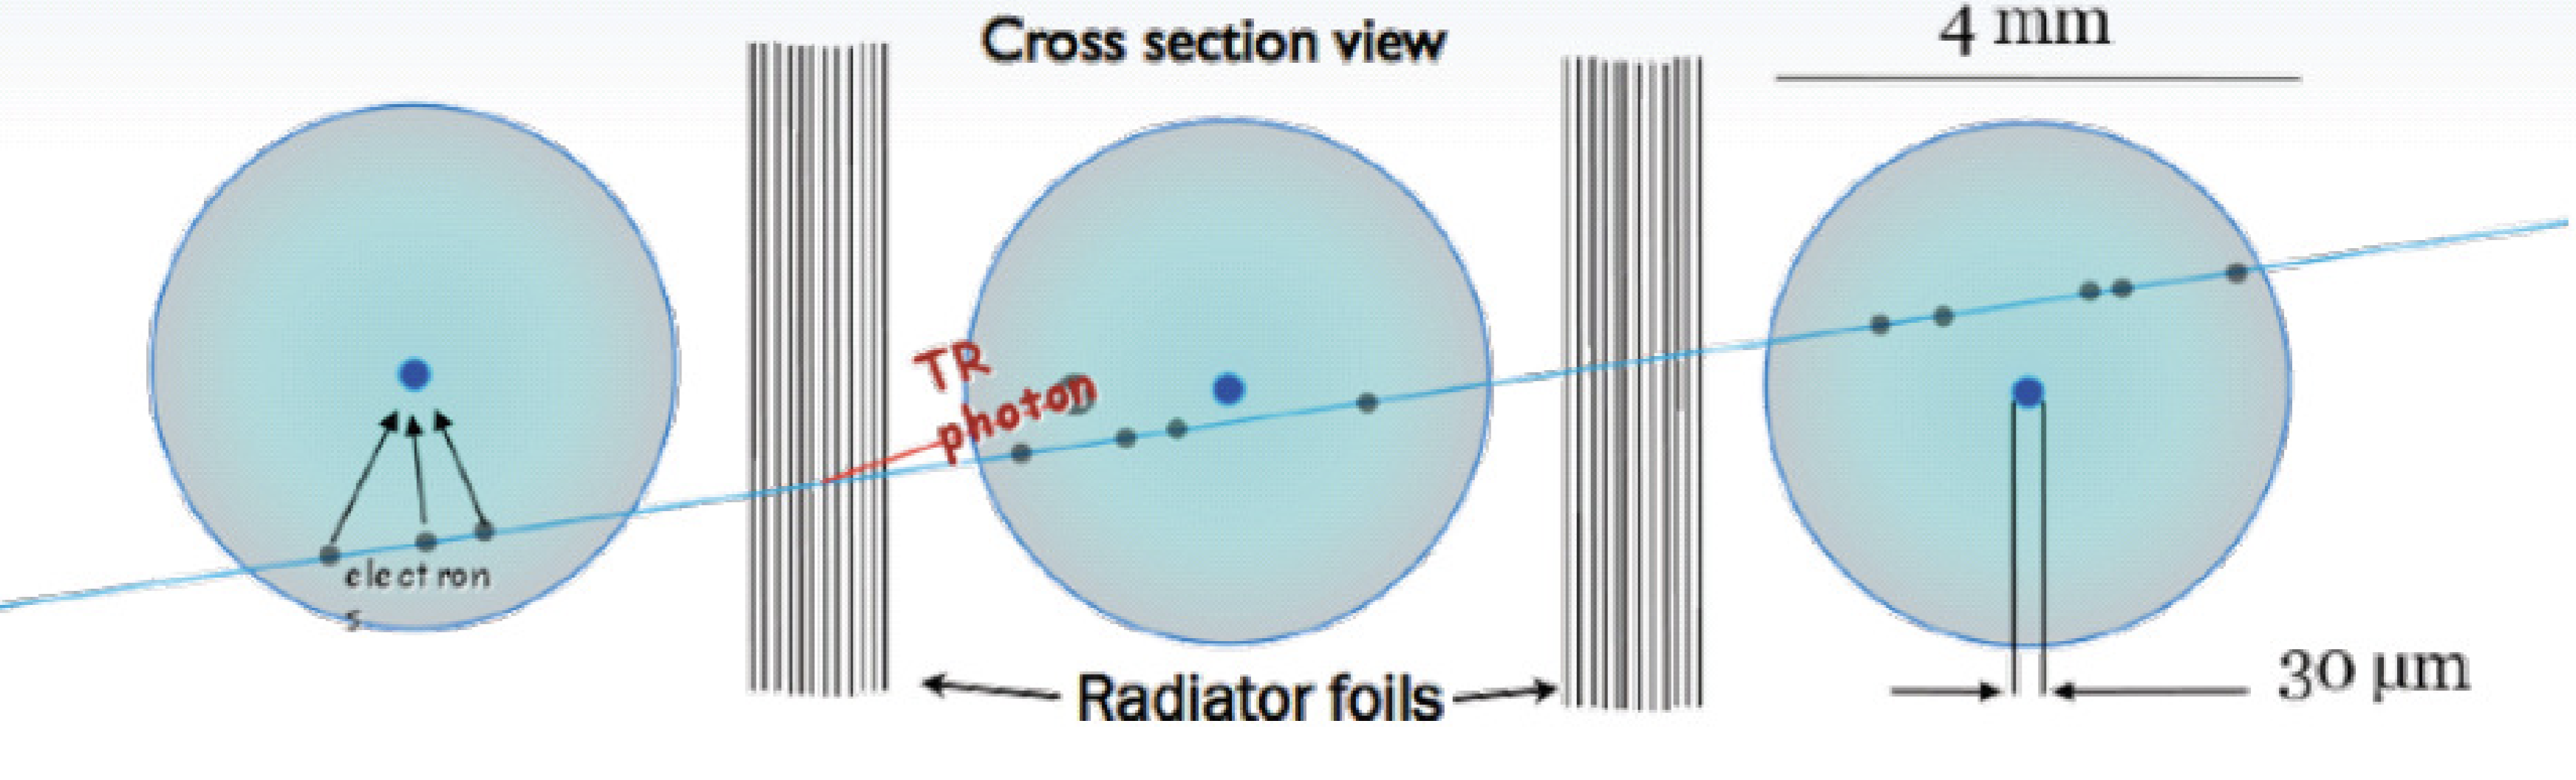
\includegraphics[width=0.8\textwidth]{figures/atlas/atlas_trt_tubes.png}
    \caption{A cross sectional view of the TRT with a particle passing through several straws is depicted. Shown is a particle ionizing the gas at it passes through the straws, creating free electrons. Additionally shown is transition radiation
    that is produce via a particle traversing the foils. Taken from~\cite{atlas_trt}}\label{fig:atlas_trt_straw_hits}
\end{figure}

Similarly to the other sub-detectors, the TRT consists of a barrel and two end-cap regions. The barrel consists of approximately 100,000 straw tubes of length 144 cm, that are laid parallel to the beam axis, arranged in 73 layers, and covers the range of $|\eta| < 1$. In contrast, each end-cap consists of approximately 120,000 straw tubes that are 39 cm in length, oriented in the radial direction, with 160 layers, and covers the range of $1 < |\eta| < 2$. On average, a charged particle is expected to cross 30 straws. The barrel and end-cap schematics can be seen in Figure~\ref{fig:atlas_id} and Figure~\ref{fig:atlas_id_endcap} respectively.

\subsection{Calorimeter}\label{sec:atlas_calorimeter}
% The ATLAS calorimeter system~\cite{atlas_calorimeter_tdr}, shown in Figure~\ref{fig:atlas_calorimeter}, is the next major sub-system of the ATLAS detector, and is designed to measure the energy of all particles, excluding muons and neutrinos, that traverse it in the pseudorapidity range of $|\eta| < 4.9$\@. The calorimeter system is split into three sub-detectors: the Electromagnetic Calorimeter (ECal), the Hadronic Calorimeter (HCal), and the Forward Calorimeter (FCal). 

% The ECal is the innermost layer of the calorimeter system and surrounds the ID\@. It consists of a barrel section and two end-caps, and its primary function is to measure the energy of electromagnetic particles, such as electrons and photons. The HCal surrounds the ECal and is designed to measure energy deposited by hadrons, jets, taus and missing transverse energy (\met). Finally, the FCal, is located in the very forward region between the hadronic end-caps and the beam pipe. The FCal includes both electromagnetic and hadronic components and extends the detector acceptance in the high $|\eta|$ region.

% Particles deposit energy in the calorimeter in different ways depending on their type. Electrons, for example, lose energy primarily via bremsstrahlung radiation, while photons primarily lose their energy via pair production when passing through the passive material in the ECal. These interactions occur over a characteristic distance known as the radiation length \radlength, which is defined as the average distance over which a high energy particle loses all but 1/$e$ (37\%) of its energy. The radiation length depends on the material and is given empirically by equation~\ref{eq:rad_length}:

% \begin{equation}
%     \centering
%     X_{0} = 716.4 \ \mathrm{g \ cm^{-2} \ \frac{A}{Z (Z+1) \ln{\frac{287}{\sqrt{Z}}}}}
%     \label{eq:rad_length}
% \end{equation}

% \noindent{}where $A$ is the atomic mass number and $Z$ is the atomic number of the absorber material. A small radiation length is desirable in the ECal to ensure that the electromagnetic showers are contained within this detector.

% Hadrons, in contrast, lose energy primarily through inelastic interactions with nuclei in the absorber material. These interactions produce secondary particles, leading to a hadronic shower. The amount of particles remaining after traveling a distance $x$ through a material is given by equation~\ref{eq:hadronic_num_remaining}:

% \begin{equation}
%     \centering
%     N(x) = N_{0} e^{-\frac{x}{\lambda}}
%     \label{eq:hadronic_num_remaining}
% \end{equation}

% \noindent{}where $N_{0}$ is the initial number incoming particles, and $\lambda$ is the nuclear interaction length, defined as:

% \begin{equation}
%     \centering
%     \lambda_{a} = 35 \ \mathrm{g \ cm^{-2}} \ A^{\frac{1}{3}}
%     \label{eq:absorption_length}
% \end{equation}

% \noindent{}This length is the average distance a hadron travels before under-going a nuclear interaction. Lighter materials with small $A$ have smaller interaction lengths, resulting in more interactions, and therefore are more suitable for the HCal\@.

% The ATLAS calorimeters use different technologies depending on their purpose. The ECal and the end-cap regions of the HCal and FCal are based on liquid argon (LAr) technology. The central barrel of the HCal uses a scintillating Tile calorimeter, where the absorber is steel, and the active material is a plastic scintillator. All of the calorimeters are sampling calorimeters, meaning they are composed of alternating layers of absorber and active materials.

% \begin{figure}
%     \centering
%     \includegraphics[width=0.8\textwidth]{figures/atlas/atlas_calorimeter.jpg}
%     \caption{Cut away view of the ATLAS calorimeter system is depicted. The first layer of the calorimeter is the EM calorimeter, surrounded by the hadronic calorimeter. Taken from~\cite{atlas_tile_calorimeter}}\label{fig:atlas_calorimeter}
% \end{figure}


%%%%%%%%%%%%%%%% Revision

The ATLAS calorimeter system~\cite{atlas_calorimeter_tdr} measures the energy of all particles except muons and neutrinos within the pseudorapidity of $|\eta| < 4.9$\@. It consists of three sub-detectors: the Electromagnetic Calorimeter (ECal), the Hadronic Calorimeter (HCal), and the Forward Calorimeter (FCal). 

The ECal surrounds the ID and measures the energy of electrons and photons and consists of a barrel and two end-caps. The HCal surrounds the ECal and measures energy deposited by hadrons, jets, taus and missing transverse energy (\met). The FCal is located in the very forward region between the hadronic end-caps and the beam pipe extending the $|\eta|$ region and has both EM and hadronic components. 

Electrons primarily lose energy via bremsstrahlung radiation, while photons primarily lose their energy via pair production when passing through the passive material in the ECal. These interactions occur over a characteristic radiation length \radlength, defined as the average distance in which high energy particle loses all but 1/$e$ (37\%) of its energy. The \radlength{} depends on the material and is given empirically by

\begin{equation}
    \centering
    X_{0} = 716.4 \ \mathrm{g \ cm^{-2} \ \frac{A}{Z (Z+1) \ln{\frac{287}{\sqrt{Z}}}}}
    \label{eq:rad_length}
\end{equation}

\noindent{}where $A$ is the atomic mass number and $Z$ the atomic number of the absorber material. A small radiation length is ideal for the ECal to ensure that the EM shower is contained.

Hadrons primarily lose energy through inelastic interactions with nuclei in the absorber material. These interactions produce secondary particles resulting in a hadronic shower. The amount of particles remaining after traveling a distance $x$ is given by $N(x) = N_{0} e^{-\frac{x}{\lambda}}$ where $N_{0}$ is the initial number incoming particles, and $\lambda$ is the nuclear interaction length, defined as:

\begin{equation}
    \centering
    \lambda_{a} = 35 \ \mathrm{g \ cm^{-2}} \ A^{\frac{1}{3}}
    \label{eq:absorption_length}
\end{equation}

\noindent{} where $\lambda$ represents the average distance a hadron travels before under going a nuclear interaction. Light materials with small $A$ have more interactions and therefore are more suitable for the HCal\@.

The calorimeters use different technologies depending on their purpose. The ECal, HCal end-caps, and FCal use liquid argon (LAr) while the center barrel of the HCal uses steel-scintillator Tile. All calorimeters are sampling calorimeters since they are composed of alternating layers of absorber and active materials.

\begin{figure}
    \centering
    \includegraphics[width=0.8\textwidth]{figures/atlas/atlas_calorimeter.jpg}
    \caption{Cut away view of the ATLAS calorimeter system is depicted. The first layer of the calorimeter is the EM calorimeter, surrounded by the hadronic calorimeter. Taken from~\cite{atlas_tile_calorimeter}}\label{fig:atlas_calorimeter}
\end{figure}
\subsubsection{Electromagnetic Calorimeter}\label{sec:atlas_em_calorimeter}
% \begin{figure}[htp]
%     \centering
%     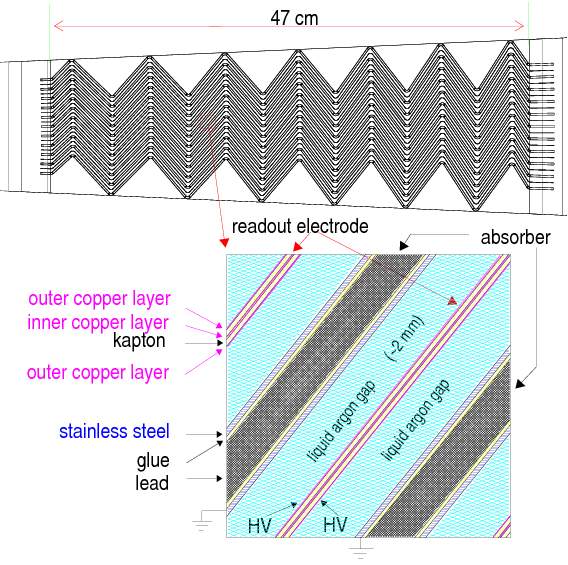
\includegraphics[width=0.5\textwidth]{figures/atlas/atlas_larg_module_accordion.png}
%     \caption{Schematic for the accordion geometry (upper) of the LAr module, shown in a plane transverse to the LHC\@. Additionally, the layout of the readout electronics (bottom) is depicted, showing the liquid argon gaps and lead absorbers. This depicts the sampling architecture of the calorimeter nicely. Taken from~\cite{atlas_calorimeter_module_accordion}}\label{fig:atlas_calorimeter_accordion}
% \end{figure}

% The ECal is the inner most layer of the calorimeter system, surrounding the entire ID\@. As mentioned in the previous section, the ECal is a LAr based calorimeter where the active material is liquid argon and the passive absorbers are lead plates. Lead absorbers are chosen due to the high atomic number of the material resulting in a small $X_0$. The barrel region ($|\eta| < 1.475$) consists of two half barrels centered around the beam axis, with each half barrel consisting of 16 modules. The half barrels are separated from one another at $z = 0$ with a 4 mm gap. Each end-cap consists of two co-axial wheels, that are divided into eight modules, and cover the region $1.375 < |\eta| < 3.2$. Between the IP and calorimeter, there is approximately 1.7 \radlength, so to account for possible energy loss by electrons and photons a liquid-argon pre-sampler with resolution $\Delta\varphi \times \Delta\eta = 0.1 \times 0.025$ is placed in front of calorimeters in the range $|\eta| < 1.8$, allowing for an improved energy measurement. In the barrel and end-caps of the ECal, the lead absorbers and electrodes are accordion in shape, allowing for full coverage in $\varphi$. This accordion geometry, as well as the alternating pattern of liquid argon and lead, is seen in figure.~\ref{fig:atlas_calorimeter_accordion}. Overall, the ECal has a total of 180,000 readout channels. 

% A LAr module consists of three different layers, with increasing granularity as distance from the IP increases\@. The first of these layers is the strip cells which have a resolution of $\Delta\varphi \times \Delta\eta = 0.1 \times 0.0031$, and extends for 4.3 \radlength{} before the second layer. The second layer consists of square cells with a resolution of $\Delta\varphi \times \Delta\eta = 0.025 \times 0.025$, and extends for at least 16.0 \radlength{} before reaching the third layer. This is the primary energy-depositing layer where the majority of the EM shower is absorbed. The third layer consists of coarser cells with a resolution of $\Delta\varphi \times \Delta\eta = 0.025 \times 0.05$, spanning approximately 2 \radlength. It is important to note that these \radlength{} correspond to $\eta = 0$ but differ depending on barrel $\eta$. Additionally, the third layer consists of even larger cells with a resolution of $\Delta\varphi \times \Delta\eta = 0.1 \times 0.1$, known as ``Trigger Towers'' (TTs), which were used in the Level-1 (L1) trigger system during the first two runs. For Run 3, the TT's are replaced\footnote{Technically, the TT's were not replaced but were supplemented with another technology that was meant to replace them eventually. The TT's were finally turned off in the middle of data taking in 2024.} with the new SuperCells that provide a more granular resolution. A comparison between the TT's and SuperCells can be seen in Figure~\ref{fig:atlas_super_cells}. Unlike the TT's, the SuperCells consists of four layers of varying granularity. The first layer (Layer 0), corresponding to the pre-sampler, has the same granularity as TT's of $\Delta\varphi \times \Delta\eta = 0.1 \times 0.1$. Layers 1 and 2 have a granularity as small as $\Delta\varphi \times \Delta\eta = 0.025 \times 0.1$, and the final layer returns to $\Delta\varphi \times \Delta\eta = 0.1 \times 0.1$. These changes allow for improved trigger algorithms, and provide a better definition of energy showers in the calorimeter. The trigger system will be discussed in more detail in Section~\ref{sec:atlas_trigger}. A sketch of a barrel module with the different layers can be seen in Figure~\ref{fig:atlas_calorimeter_module}.

% \begin{figure}[htp]
%     \centering
%     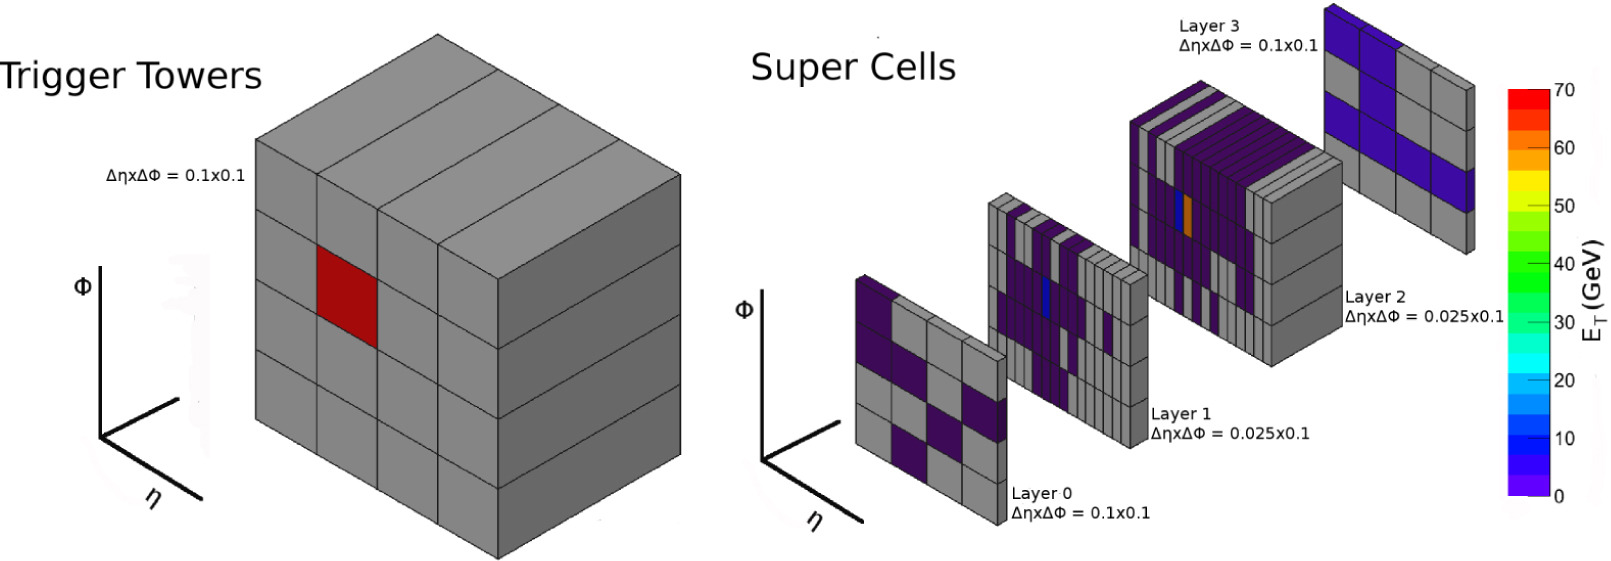
\includegraphics[width=0.8\textwidth]{figures/atlas/atlas_calorimeter_tt_to_supercell.jpg}
%     \caption{A schematic comparison between a TT (left) and a SuperCell (right). The TT has a fixed granularity while the SuperCell has varying granularity allowing for more complex trigger algorithms. Taken from~\cite{atlas_calorimeter_supercell}}\label{fig:atlas_super_cells}
% \end{figure}

% \begin{figure}[htp]
%     \centering
%     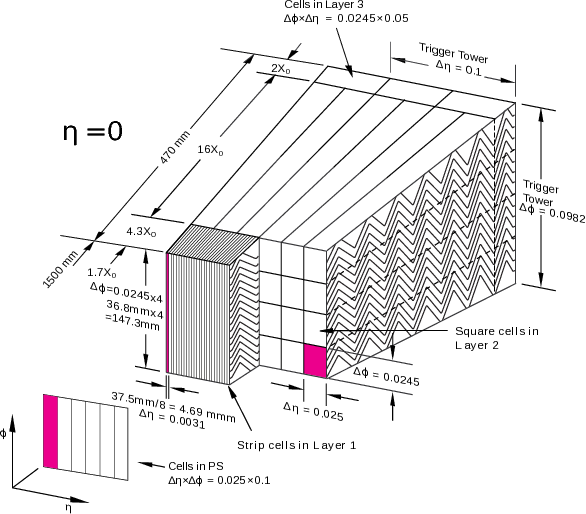
\includegraphics[width=0.7\textwidth]{figures/atlas/atlas_lar_module_cells.png}
%     \caption{A sketch of a barrel module with its three different layers. The first layer consists of very granular strip cells, the second layer consists of square cells, and the third layer consists of slightly larger cells then the second layer. Taken from~\cite{atlas_calorimeter_module_accordion}}\label{fig:atlas_calorimeter_module}
% \end{figure}
%%%%%%%%%%%%%%%%%% Revision

The ECal is the innermost layer of the calorimeter system, surrounds the ID and uses LAr as active material and lead as its passive. Lead absorbers are chosen for their high atomic number resulting in a small $X_0$. 

The barrel region ($|\eta| < 1.475$) consists of two half barrels each with 16 modules and are separated by a 4 mm gap at $z = 0$. Each end-cap covers $1.375 < |\eta| < 3.2$ with two co-axial wheels split into eight modules. A liquid-argon pre-sampler with resolution $\Delta\varphi \times \Delta\eta = 0.1 \times 0.025$ is placed in front of the calorimeter and covers $|\eta| < 1.8$ to correct for the energy loss due to the 1.7 \radlength{} between the IP and calorimeter. 

Combined, the barrel and end-caps of the ECal contain 180,000 readout channels and have the lead absorbers and electrodes in accordion shapes, allowing for full coverage in $\varphi$. The accordion geometry and sampling calorimeter nature can be seen in Figure~\ref{fig:atlas_calorimeter_accordion}. 

\begin{figure}[htp]
    \centering
    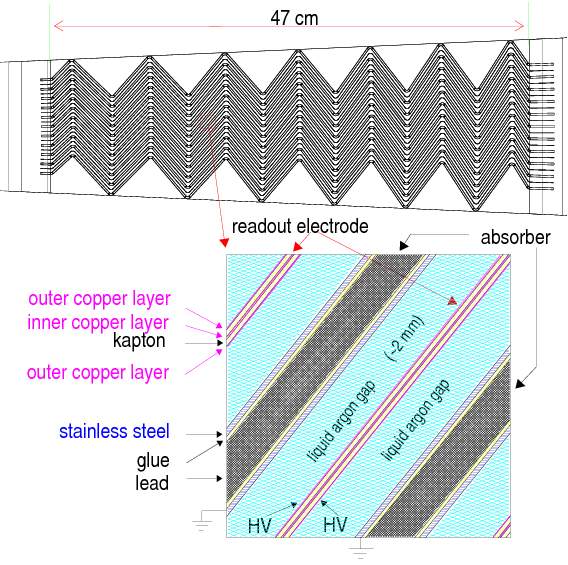
\includegraphics[width=0.55\textwidth]{figures/atlas/atlas_larg_module_accordion.png}
    \caption{Schematic for the accordion geometry (upper) of the LAr module, shown in a plane transverse to the LHC\@. Additionally, the layout of the readout electronics (bottom) is depicted, showing the liquid argon gaps and lead absorbers. This depicts the sampling architecture of the calorimeter nicely. Taken from~\cite{atlas_calorimeter_module_accordion}}\label{fig:atlas_calorimeter_accordion}
\end{figure}

\begin{figure}[htp]
    \centering
    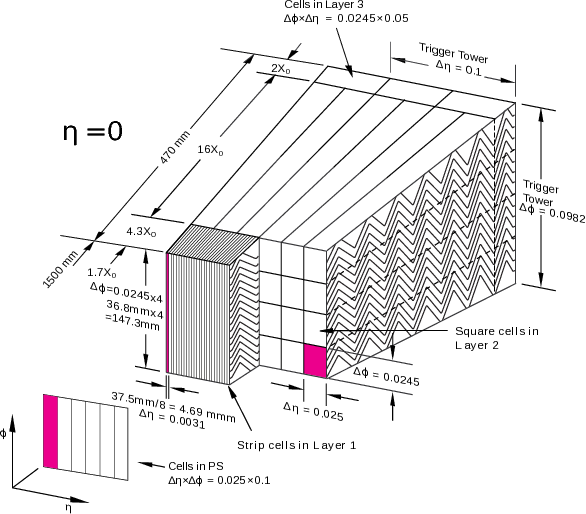
\includegraphics[width=0.6\textwidth]{figures/atlas/atlas_lar_module_cells.png}
    \caption{A sketch of a barrel module with its three different layers. The first layer consists of very granular strip cells, the second layer consists of square cells, and the third layer consists of slightly larger cells then the second layer. Taken from~\cite{atlas_calorimeter_module_accordion}}\label{fig:atlas_calorimeter_module}
\end{figure}

The LAr modules, as seen in Figure~\ref{fig:atlas_calorimeter_module}, consist of three layers with decreasing granularity as distance from the IP increases:
\begin{itemize}
    \setlength\itemsep{0em}
    \setlength\parskip{0pt}
    \item Layer 1: Strip cells with resolution $\Delta\varphi \times \Delta\eta = 0.1 \times 0.0031$, spans 4.3 \radlength{}
    \item Layer 2: Square cells with resolution $\Delta\varphi \times \Delta\eta = 0.025 \times 0.025$, spans at least 16.0 \radlength{}
    \item Layer 3: Coarser cells with resolution $\Delta\varphi \times \Delta\eta = 0.025 \times 0.05$, spans approximately 2 \radlength{}
\end{itemize}

The given \radlength{} correspond to $\eta = 0$ but differ depending on barrel $\eta$. Additionally, the third layer consists of Trigger Towers (TTs) with a resolution of $\Delta\varphi \times \Delta\eta = 0.1 \times 0.1$, which were used in the Level-1 (L1) in Runs 1--2. In Run 3, they have been replaced\footnote{TTs were initially supplemented by these, but have since been disabled in 2024.} by SuperCells as shown in Figure~\ref{fig:atlas_super_cells}, which have four layers of varying granularity:
\begin{itemize}
    \setlength\itemsep{0em}
    \setlength\parskip{0pt}
    \item Layer 0: Pre-sampler with resolution $\Delta\varphi \times \Delta\eta = 0.1 \times 0.1$
    \item Layers 1,2: Resolution $\Delta\varphi \times \Delta\eta = 0.025 \times 0.1$
    \item Layer 3: Resolution $\Delta\varphi \times \Delta\eta = 0.1 \times 0.1$.
\end{itemize}
These changes allow for better trigger resolution and shower shape discrimination. The trigger will be discussed in more detail in Section~\ref{sec:atlas_trigger}.

\begin{figure}[htp]
    \centering
    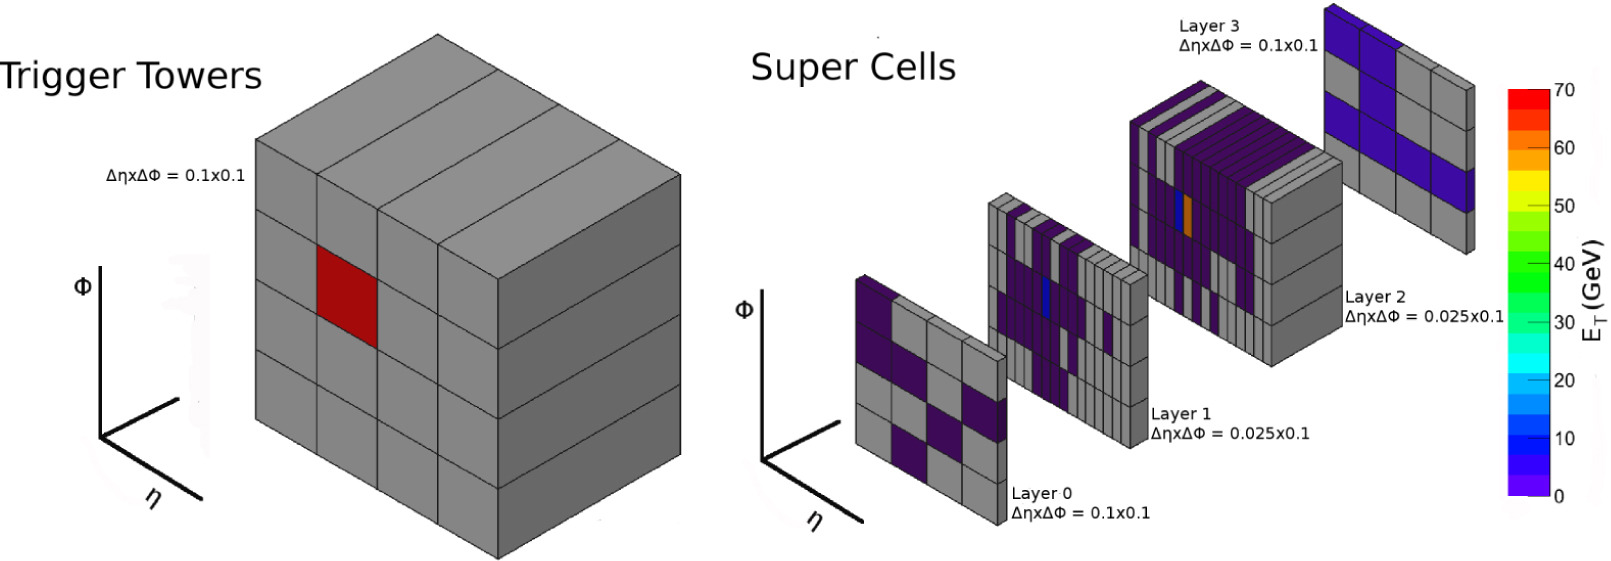
\includegraphics[width=0.8\textwidth]{figures/atlas/atlas_calorimeter_tt_to_supercell.jpg}
    \caption{A schematic comparison between a TT (left) and a SuperCell (right). The TT has a fixed granularity while the SuperCell has varying granularity allowing for more complex trigger algorithms. Taken from~\cite{atlas_calorimeter_supercell}}\label{fig:atlas_super_cells}
\end{figure}
\subsubsection{Hadronic Calorimeter}\label{sec:atlas_had_calorimeter}
% The HCal is the outer most part of the calorimeter and consists of two different detector technologies: the scintillating Title calorimeter (TileCal) in the barrel region, and the LAr based calorimeters in the end-caps\@.

% The TileCal uses steel as the absorber material and plastic scintillator as the active medium. It covers the region $|\eta| < 1.7$ and is composed of a central barrel and two extended barrels, as shown in Figure~\ref{fig:atlas_calorimeter}. Between the central and extended barrels lies a gap region, which is instrumented with special steel-scintillator modules designed to partially recover energy lost in this area. Each barrel consists of 64 modules, each spanning approximately $\Delta\varphi = 0.1$. The modules are constructed with alternating layers of steel plates and scintillating tiles, with a volume ratio of about 4.7:1 in favor of steel. The absorbers provide approximately 7.4\intlength{}.

% As hadrons traverse the absorber, they interact with nuclei in the material, initiating hadronic showers. These showers pass through the scintillating tiles, producing ultraviolet photons. The UV photons are then converted to visible light by special wavelength-shifting fibers, which transmit the photons to photomultiplier tubes (PMTs) for signal readout. A schematic of a TileCal module is shown in Figure~\ref{fig:atlas_hcal_module}.

% \begin{figure}[htp]
%     \centering
%     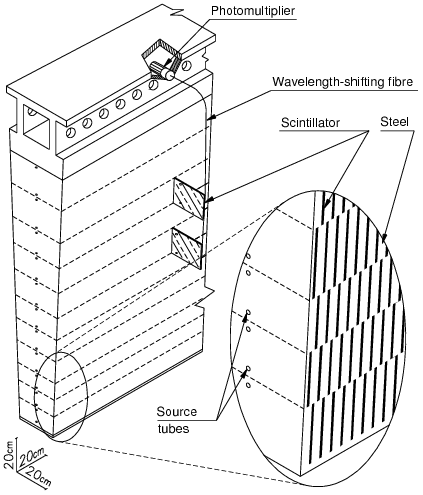
\includegraphics[width=0.5\textwidth]{figures/atlas/atlas_hcal_module.png}
%     \caption{Schematic of a TileCal module illustrating the sampling structure of alternating steel absorbers and scintillating tiles. The optical readout system, including wavelength-shifting fibers and PMTs, is also shown. Taken from~\cite{atlas_collaboration_paper}.}\label{fig:atlas_hcal_module}
% \end{figure}

% The hadronic end-cap calorimeters (HEC) are a copper and liquid-argon sampling detector covering the range $1.5 < |\eta| < 3.2$. The HEC consists of two wheels in each end-cap with the front wheel (HEC1) and a rear wheel (HEC2) with each wheel consisting of 32 identical wedge-shaped modules. The modules in HEC1 consist of 24 copper plates with thickness 25 mm and a 12.5 mm thick front plate. The modules in HEC2 consist of 16 copper plates with thickness 50 mm, and front plate thickness of 25 mm. The gaps between the plates is where the active material, LAr, is located. These gaps have a thickness of 8.5 mm. The LAr gaps are further split by three electrodes creating four separate drift zones of 1.8 mm, and is shown in Figure~\ref{fig:atlas_hcal_endcap_module}.

% \begin{figure}[htp]
%     \centering
%     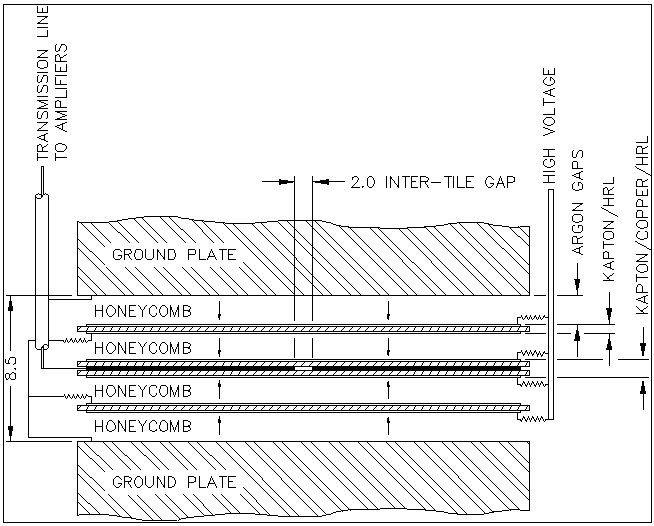
\includegraphics[width=0.7\textwidth]{figures/atlas/atlas_hcal_endcap_module.png}
%     \caption{Schematic of a HEC module showing the LAr region between two copper absorber plates, subdivided into four drift zones by embedded electrodes. Taken from~\cite{atlas_collaboration_paper}.}\label{fig:atlas_hcal_endcap_module}
% \end{figure}

%%%%%%%%%%%%%%%% revision
The HCal is the outermost part of the calorimeter and uses two detector technologies: the scintillating Tile calorimeter (TileCal) in the barrel region, and the LAr based calorimeters in the end-caps\@.

The TileCal covers $|\eta| < 1.7$ and consists of a central barrel and two extended barrels separated by a gap region that is instrumented with special modules to recover lost energy. Each barrel includes 64 modules that span approximately $\Delta\varphi = 0.1$ and are built from alternating layers of steel plates and scintillating tiles in a 4.7:1 volume ratio, where the steel plates provide approximately 7.4\intlength{}. As hadrons shower, they pass through the scintillating tiles and produce UV photons that are converted to visible light by special wavelength-shifting fibers, which transmit the photons to photomultiplier tubes (PMTs) for signal readout. A TileCal module is shown in Figure~\ref{fig:atlas_hcal_module}.

\begin{figure}[htp]
    \centering
    \subfloat[TileCal module.]{%
        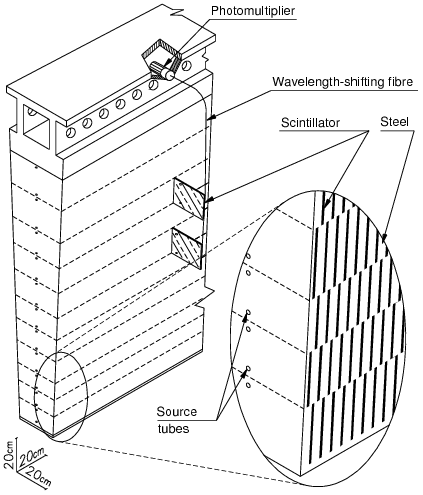
\includegraphics[width=0.45\textwidth]{figures/atlas/atlas_hcal_module.png}\label{fig:atlas_hcal_module}
    }
    \hfill
    \subfloat[HEC module.]{%
        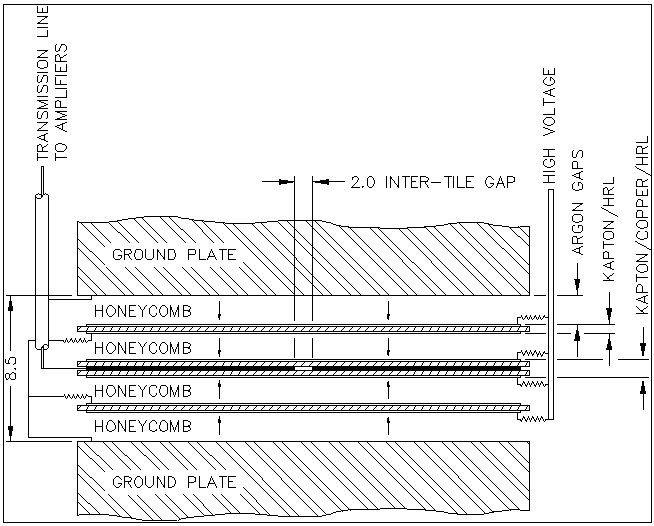
\includegraphics[width=0.45\textwidth]{figures/atlas/atlas_hcal_endcap_module.png}\label{fig:atlas_hcal_endcap_module}
    }
    \caption{Schematic structure of the ATLAS hadronic calorimeters: (a) TileCal and (b) HEC\@. Figures from~\cite{atlas_collaboration_paper}.}\label{fig:atlas_hcal_combined}
\end{figure}

The hadronic end-cap calorimeters (HEC) cover $1.5 < |\eta| < 3.2$ and consist of two LAr-copper sampling wheels per end-cap separated by LAr gap of 8.5 mm.  The front wheel (HEC1) consists of 32 identical wedge-shaped modules each containing 24 copper plates of 25 mm thickness and a 12.5 mm thick front plate while the second wheel (HEC2) consist of 16 copper plates of 50 mm thickness and a 25 mm thick front plate. Each LAr gap is divided into four 1.8 mm drift zones by embedded electrodes as shown in Figure~\ref{fig:atlas_hcal_endcap_module}.
 
\subsubsection{Forward Calorimeter}\label{sec:atlas_fcal}
The FCal is the final part of the calorimeter system and is located between the end-cap calorimeters and the beam pipe. It covers the psuedorapidity of $3.1 < |\eta| < 4.9$ and is composed of three longitudinal sections: FCal1, FCal2, and FCal3 as shown in Figure~\ref{fig:forward_detector_layout}. 

\begin{figure}[htp]
    \centering
    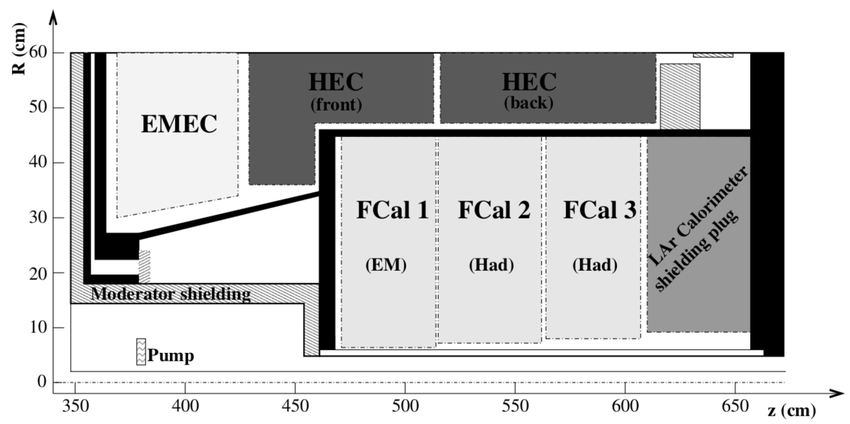
\includegraphics[width=0.8\textwidth]{figures/atlas/atlas_fcal_breakdown.png}
    \caption{The layout of the forward calorimeter system. Depicted are the three different layers with the FCal1 being a ECal, while the FCal2 and FCal3 are HCals. Taken from~\cite{atlas_collaboration_paper}}\label{fig:forward_detector_layout}
\end{figure}

FCal1 is a LAr based ECal, that uses copper absorber material to optimize both heat removal and energy resolution. It provides a total of 27.6 \radlength{}. The structure consists of longitudinally stacked copper plates with holes drilled in them for the electrodes. Each electrode is co-axial structure consisting of an inner copper rod and an outer copper tube, separated by a plastic fiber containing the liquid argon. The electrode structure can be seen in Figure~\ref{fig:atlas_fcal_electrode}. 

\begin{figure}[htp]
    \centering
    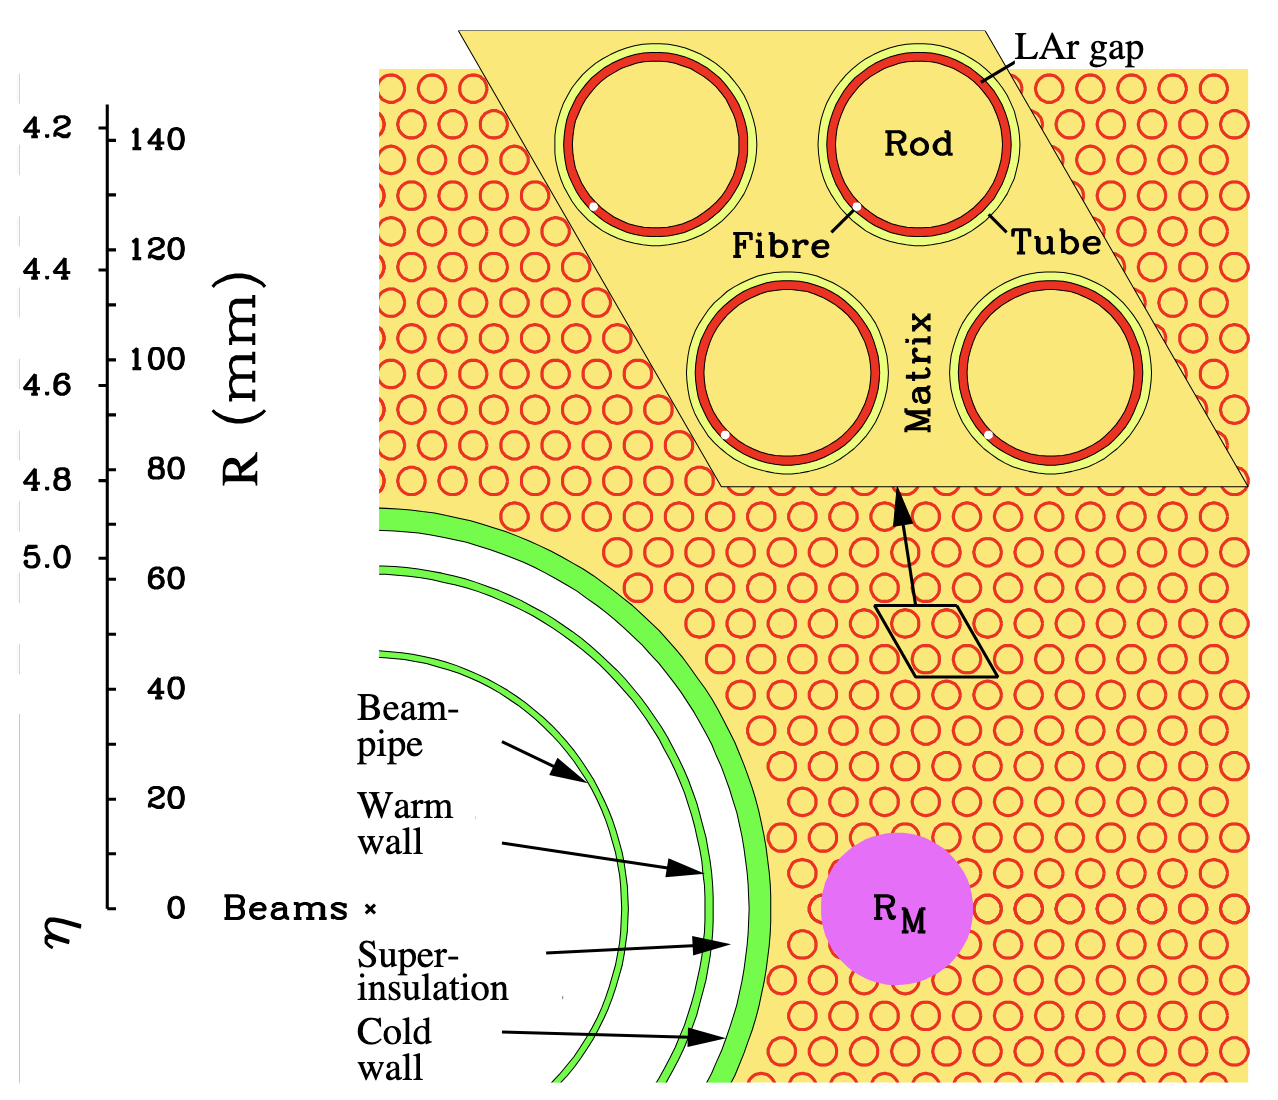
\includegraphics[width=0.6\textwidth]{figures/atlas/atlas_fcal_electrode.png}
    \caption{Electrode structure with FCal1 with the matrix of copper plates and copper tubes. This figure also applies to FCal2 and FCal3 with the copper rods being replaced with tungsten rods. Taken from~\cite{atlas_collaboration_paper}}\label{fig:atlas_fcal_electrode}
\end{figure}

FCal2 and FCal3 are LAr based HCals, optimized for a high absorption length (3.68 \intlength{} and 3.60 \intlength{} respectively) by maximizing the amount of tungsten used in the modules. The modules are designed similarly to FCal1 with the only exception being that the rod is made of tungsten instead of copper. 

To minimize contamination from unabsorbed particles in the muon system, a shielding plug is downstream from FCal3.


\subsection{Muon Spectrometer}\label{sec:atlas_muon}
% The outermost part of the ATLAS detector is the Muon Spectrometer (MS), designed to detect charged particles that escape the ID and calorimeter, and to measure their momentum in the pseudorapidity range of $\eta < 2.7$. Due to their relatively large mass, muons are less affected by bremsstrahlung radiation, and are typically the only particle to reach the MS\@. The MS was designed with two primary objectives: precise momentum measurements (resolution $\leq 50 ~\mu$m) and a fast muon trigger (15--25 ns). To achieve this, the MS uses five different gas-based detectors: The Monitored Drift Tube~\cite{atlas_mdt_paper} (MDT) chambers, the Resistive Plate Chambers~\cite{atlas_run3_rpc_paper} (RPC), the Thin Gap Chambers (TGC)~\cite{atlas_tgc_paper}, the Micromegas~\cite{atlas_mm_paper} (MM) and the Small-strip Thin Gap Chambers~\cite{atlas_stgc_paper} (sTGC). Refer to Figure~\ref{fig:atlas_detector} to see the layout of the MS\@.

% To obtain precision momentum measurements, the MS uses three large superconducting magnets to bend muon trajectories. MDT's are primarily used for precision momentum measurements due to their high accuracy, predictable deformations, and simplicity of construction.

% The precision-tracking chambers are complimented by a system of fast trigger chambers, which are capable of delivering tracking information with 15--25 ns after the passage of a particle. In the barrel region ($|\eta| < 1.05$) RPC's were selected for the triggering chambers, and in the end-caps ($1.05 < |\eta| < 2.4$) the TGC's were chosen. The timing resolution of the triggering detectors is finer than the LHC bunch spacing, allowing for reliable bunch crossing identification.

% For Run 3, the sTGC and MM detectors were added to the MS and are known together as the New Small Wheel (NSW). These detectors compliment both the precision tracking detectors and fast triggering capabilities, by providing additional tracking and triggering information in the end-cap region.

The outermost part of ATLAS is the Muon Spectrometer (MS), designed to detect and measure the momentum of charged particles in the range $|\eta| < 2.7$. Due to their large mass and minimum energy loss by bremsstrahlung radiation, muons are typically the only particle that enter the muon system\@. The MS was designed to provide precise momentum measurements (resolution $\leq 50 ~\mu$m) and fast muon trigger (15--25 ns). 

Precision momentum measurements are achieved through the use of a strong magnetic field described in Section~\ref{sec:atlas_magnet} and the Monitored Drift Tube~\cite{atlas_mdt_paper} (MDT) chambers which have high accuracy and predictable deformations.

Fast triggering is is achieved through the use of Resistive Plate Chambers~\cite{atlas_run3_rpc_paper} (RPC) in the barrel region ($|\eta| < 1.05$) and Thin Gap Chambers (TGC)~\cite{atlas_tgc_paper} in the end-caps ($1.05 < |\eta| < 2.4$), both capable of timing resolution finer than the LHC bunch spacing allowing for reliable bunch crossing identification. 

For Run 3, the New Small Wheel (NSW) upgrade introduced the Small-strip Thin Gap Chambers~\cite{atlas_stgc_paper} (sTGC) and Micromegas~\cite{atlas_mm_paper} (MM) detectors which enhance both the tracking and triggering capabilities in the end-cap region.


\subsubsection{Monitored Drift Tubes}\label{sec:atlas_mdt}
MDT's form the majority of the precision-tracking chambers used in the MS, covering up to $|\eta| < 2.7$, except in the innermost end-cap layer where coverage is limited to $|\eta| < 2.0$. There are approximately 1,100 MDT chambers through the entire ATLAS detector, and approximately 350,000 drift tubes. Each chamber consists of one or two multilayers, with each multilayer consisting of 3 to 4 layers of drift tubes, and each layer containing 30 to 100 tubes.

In the barrel region, MDT's are located on and between the eight coils of the barrel toroid magnets. They are arranged in three concentric cylindrical layers around the $z$-axis with inner radii of approximately 5 m, 7.5 m and 10 m. MDT chamber size increases with radial distance from the IP to maintain angular resolution\@.

In the end-cap region, MDT's are placed behind the end-cap toroid magnets. The MDT's are arranged in two large wheels located along the $z$-axis at distances of 14 m and 21.5 m. These wheels are placed perpendicular to the $z$-axis and extend radially outward.

MDT's rely on drift tubes to measure the position of charge particles. In the MS, the drift tubes are approximately 30 mm in diameter and operate with a combination of Argon (93\%) and Carbon Dioxide (7\%). As a muon passes through the tube, the gas ionizes releasing electrons that drift towards the central tungsten-rhenium wire which is kept at a 3080 V. 

A cross section view of the MDT system in the $r-z$ plane can be seen in Figure~\ref{fig:atlas_mdt_cross_section} and a diagram of an MDT chamber can be seen in Figure~\ref{fig:mdt_chamber}.

\begin{figure}[htp]
    \centering
    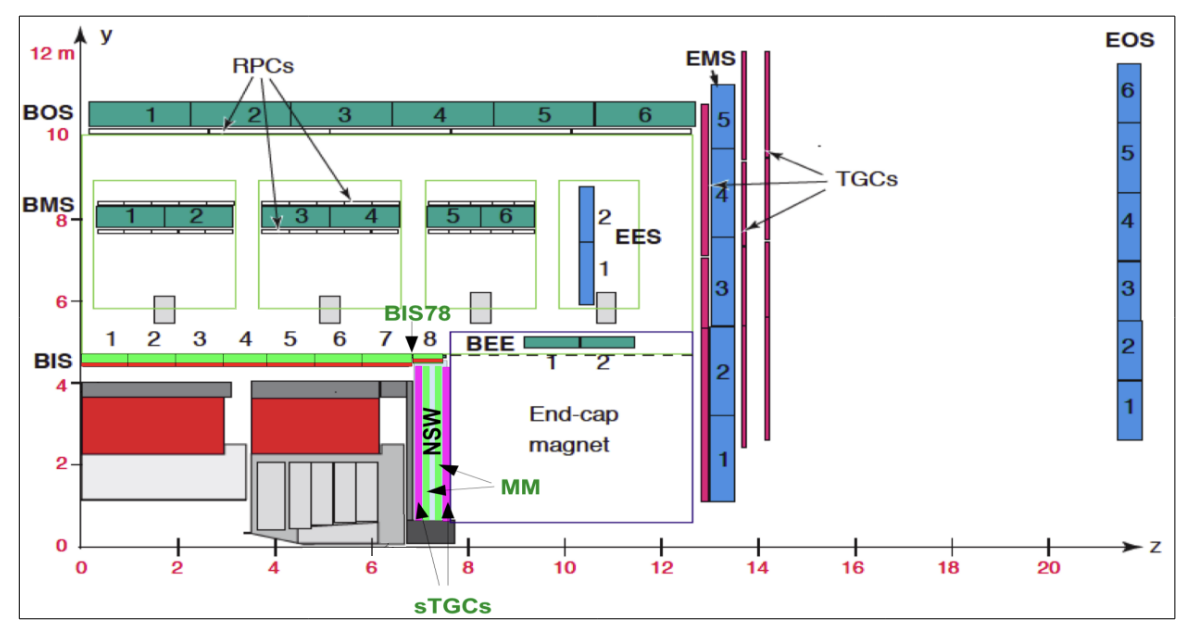
\includegraphics[width=0.8\textwidth]{figures/atlas/atlas_ms_run3_layout.png}
    \caption{Cross-section of the MDT system in the $r-z$ plane. The MDT's are located between the barrel toroid coils and the end-cap toroid coils. The MDT's are arranged in three cylindrical layers in the barrel region, and two large wheels in the end-cap region. The increasing size of the MDT's as distance from the IP increases is also seen. Taken from~\cite{atlas_mdt_cross_section}.}\label{fig:atlas_mdt_cross_section}
\end{figure}

\begin{figure}[htp]
    \centering
    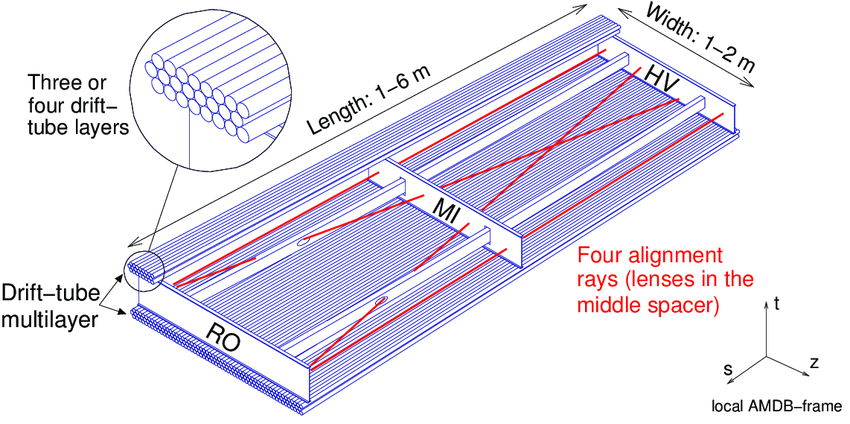
\includegraphics[width=0.8\textwidth]{figures/atlas/atlas_mdt_drifttube.png}
    \caption{Layout of a barrel MDT chamber. Drift tubes are arranged into two multilayers that are separated by a spacer. Each multilayer contains 3 or 4 layers of drift tubes. End-cap MDT chambers are trapezoidal in shape. Taken from~\cite{atlas_collaboration_paper}.}\label{fig:mdt_chamber}
\end{figure}
\subsubsection{Resistive Plate Chambers}\label{sec:atlas_rpc}
The trigger system in the barrel region depends on RPC's that are arranged in three concentric cylindrical layers about the beam axis, and are referred to as the three trigger stations. The RPC's are a gaseous parallel electrode-plate detector with no wires, consisting of two resistive plates made up phenolic-melaminic plastic laminate separated from one another by 2 mm using insulating spacers. An electric field of approximately 4.9 kV/mm is applied between the plates causing ionized particles or free electrons to accelerate towards the anode. These particles gain energy, ionizing other particles creating a so-called avalanche effect. The resulting signal is readout via capacitive coupling to metallic strips mounted on the outer surface of the plates. At the nominal operating voltage of 9.8 kV, the typical signal width is about 5 ns. The full RPC system includes approximately 3,800 gas volumes and 385,000 readout channels. The gas mixture used in the RPC's consist of $C_2H_2F_4$ (94.7\%), Iso-$C_4H_{10}$ (5\%), and $SF_6$ (0.3\%) due to their low operating voltage, non-flammability and low costs, while maintaining a stable avalanche response. In the middle and outer layers of the barrel region, RPC's and positioned around the MDT's. The middle layer, RPC's are positioned both in front of, and behind the MDT's, while the outer layer they are positioned either in front (small chamber) or behind (large chamber). A diagram of this can be seen in Figure~\ref{fig:atlas_mdt_rpc_sandwich}.

\begin{figure}[htp]
    \centering
    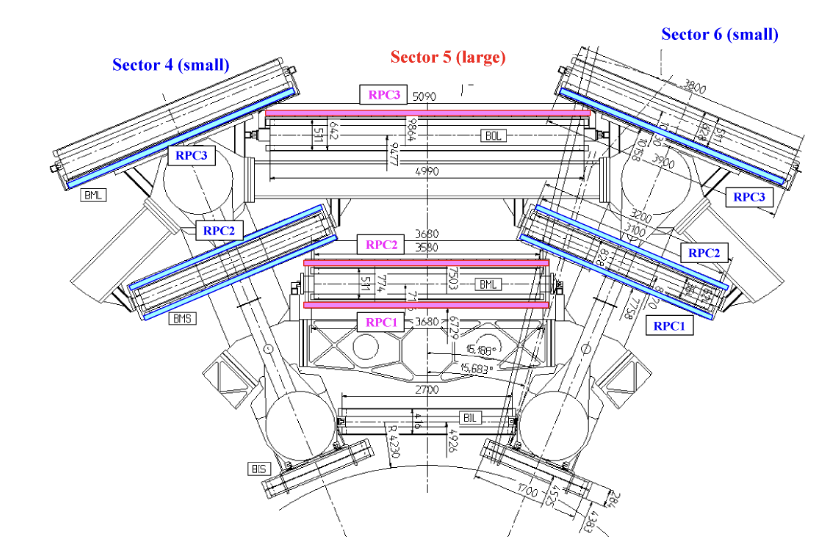
\includegraphics[width=0.8\textwidth]{figures/atlas/atlas_mdt_rpc_sandwich.png}
    \caption{Layout of the RPC and MDT system in the barrel region. The RPC's are placed in front of and behind the MDT's in the middle layer, and either in front of or behind the MDT's in the outer layer. Taken from~\cite{atlas_collaboration_paper}.}\label{fig:atlas_mdt_rpc_sandwich}
\end{figure}

\subsubsection{Thin Gap Chambers}\label{sec:atlas_tgc}
TGC's provide two functions in the MS end-cap region\@: fast muon triggering ability and the measurement of the azimuthal coordinate to complement the precise radial measurements of the MDT's. Covering the pseudorapidity range of $1.05 < |\eta| < 2.4$, the TGC's are arranged in seven detector layers that sandwich the MDT chambers. Each TGC consists of several gas volumes that contain a wire plane and two cathode planes, which is referred to as a chamber. The seven detector layers are grouped into a triplet (three chambers) layer and two doublet (two chambers) layers, which are referred to as a unit. These can be seen in Figure~\ref{fig:tgc_chamber}

\begin{figure}[htp]
    \centering
    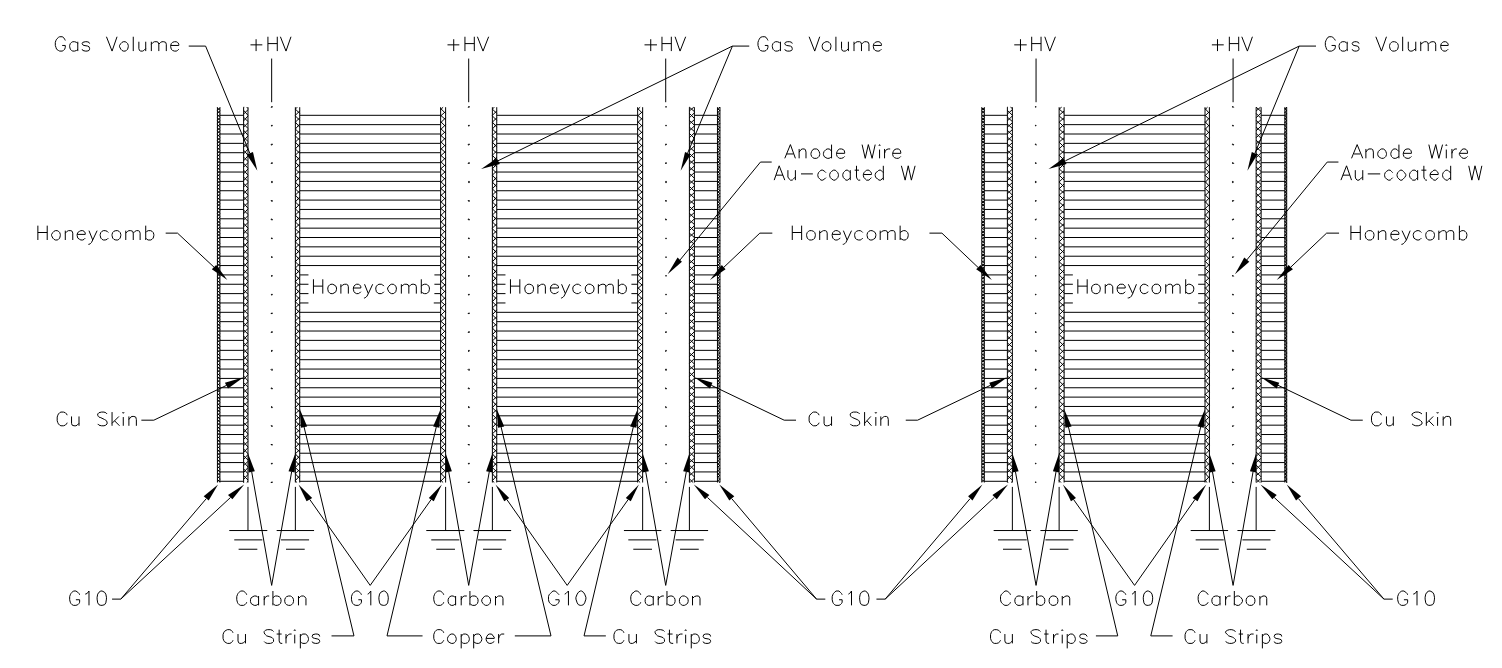
\includegraphics[width=0.8\textwidth]{figures/atlas/atlas_tgc_chamber.png}
    \caption{Cross section of a TGC triplet and doublet module. The triplet module consists of three planes of anodes, while the doublet module consists of two planes of anodes. Taken from~\cite{atlas_collaboration_paper}.}\label{fig:tgc_chamber}
\end{figure}

TGCs are multi-wire proportional chambers distinguished by a wire-to-cathode distance of 1.4 mm which is smaller than the wire-to-wire distance of 1.8 mm. This allows for excellent time resolution for most tracks. However, tracks that pass perpendicularly between the wires can have longer drift times due to the vanishing drift field. The chambers operate with a highly quenching gas mixture composed of 55\% $CO_2$ and 45\% of $n-C_5H_{12}$ allowing for operation in a quasi-saturated mode. TGC signals typically arrive within a 25 ns window with 99\% probability, allowing reliable bunch-crossing identification. The full TGC systems contains approximately 400,000 readout channels.

\subsubsection{New Small Wheel}\label{sec:atlas_nsw}
% The New Small Wheel (NSW) is a new detector system that was installed in the MS during the second long shutdown and is the first large upgrade to the ATLAS detector in preparation for the HL-LHC\@. The NSW is a set of precision tracking (Micromegas) and trigger detectors (sTGC) that are able to work at the high rates needed for the HL-LHC but also give excellent spatial and time resolution. This system consists of 16 detector planes that are arranged into two multilayers where each multilayer consists of four sTGC and four MM\@. To maximize the distance between the sTGCs for better track segment angular resolution at the trigger level, each multilayer is arranged in a sandwich configuration of sTGC-MM-MM-sTGC\@. The 16 detector sectors are subdivided into eight large sectors and 8 small sectors that alternate to ensure full cover in the $\varphi$ plane. The NSW can be seen in Figure~\ref{fig:atlas_nsw}.

% \begin{figure}[htp]
%     \centering
%     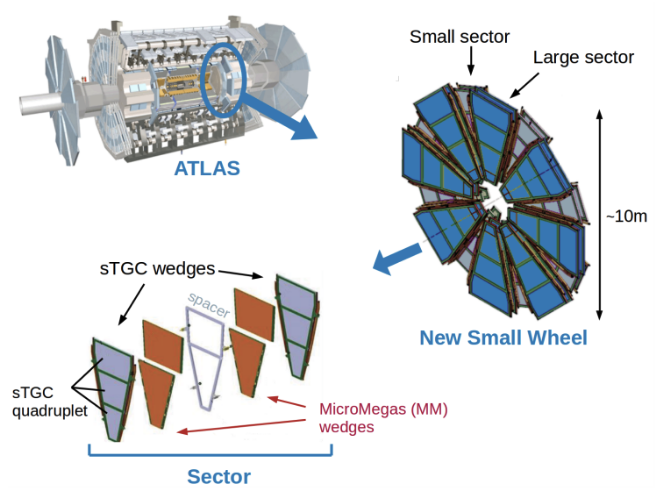
\includegraphics[width=0.65\textwidth]{figures/atlas/atlas_NSW.png}
%     \caption{Depicted is the NSW and its placement within the ATLAS detector. The figure illustrates the division of the NSW into 16 sectors, alternating between large and small sectors, as well as the internal structure of each sector. The sandwich-like arrangement of the detector planes, designed to maximize the separation between the sTGC wedges for improved angular resolution, is also visible. Taken from~\cite{NSW_image}.}\label{fig:atlas_nsw}
% \end{figure}

% The sTGC's are the primary trigger detectors in the NSW\@. They are based on the same principle as the TGC's that are used throughout the muon system except with smaller readout strips. The strips in the sTGC are 3.2 mm in pitch, significantly smaller than the TGC strips, providing improved angular resolution. In addition to strips the sTGC have another readout technology, copper pads. These pads have a significantly larger pitch of about 80 mm, and are used for the identification of muon tracks that roughly point to the IP\@.

% In contrast, the MM detectors serve as the primary precision trackers for the NSW\@. Each MM consists of a drift region defined by a copper cathode and a woven metallic mesh with an applied electric field of 600 V/cm applied between these. When an charged particle crosses this volume, an electron ion pair is created which drifts towards the mesh. An anode readout is placed below the mesh separated by a 129 $\mu$m amplification volume where there is an additional electric field of 40 kV/cm. The electric field configuration in the MM guides the electron to the amplification region, where an avalanche occurs, generating a charge signal on the readout.

%%%%%%%%%%%%%%%% revision

The New Small Wheel (NSW) was installed during LS2 and is the first major upgrade to ATLAS in preparation for the HL-LHC\@. It combines precision tracking chambers (Micromegas, MM) and trigger chambers (small-strip TGC,sTGC) that are able to meet the HL-LHC high rate and resolution demands. Each NSW consists of 16 sectors (8 large, 8 small) arranged alternatively in $\varphi$, with each sector containing two multilayers in a sTGC-MM-MM-sTGC sandwich for improved angular resolution. The NSW can be seen in Figure~\ref{fig:atlas_nsw}.

\begin{figure}[htp]
    \centering
    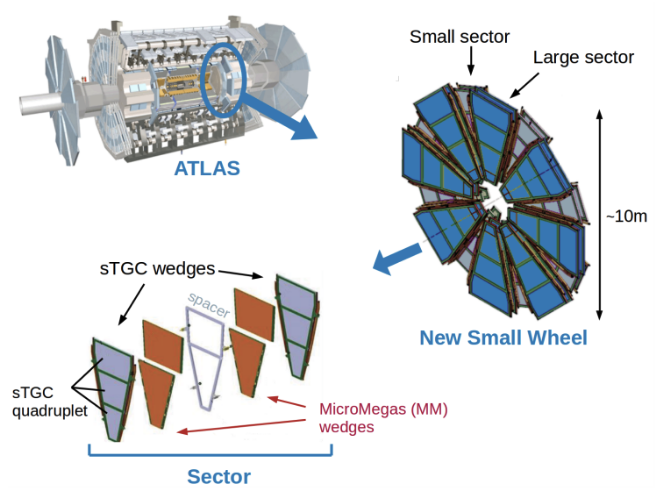
\includegraphics[width=0.65\textwidth]{figures/atlas/atlas_NSW.png}
    \caption{Depicted is the NSW and its placement within the ATLAS detector. The figure illustrates the division of the NSW into 16 sectors, alternating between large and small sectors, as well as the internal structure of each sector. The sandwich-like arrangement of the detector planes, designed to maximize the separation between the sTGC wedges for improved angular resolution, is also visible. Taken from~\cite{NSW_image}.}\label{fig:atlas_nsw}
\end{figure}

The sTGC's are the primary trigger detectors in the NSW\@. They are built upon the TGC technology but feature strips that are 3.2 mm in pitch and 80 mm copper pads for identifying muon tracks that roughly point to the IP. The MMs serve as the NSWs primary precision trackers and consist of a drift region defined by a copper cathode and a woven metallic mesh with an applied electric field of 600 V/cm. Below the mesh is an anode readout that is separated by a 129 $\mu$m amplification volume where an additional electric field of 40 kV/cm is applied. The amplification gap produces a localized avalanche signal that is read out by the anode.


\subsection{Trigger And Data Acquisition}\label{sec:atlas_trigger}
\subsubsection{Level 1 Trigger}\label{sec:atlas_l1_trigger}
The LHC collides protons at a rate of 40 MHz, producing an extraordinarily large amount of data (\~ 1.5 MB per event). Unfortunately, it is not feasible for ATLAS to record every single event that occurs because it would require storage capabilities that nowhere on Earth could provide. Instead, ATLAS employs a triggering system that reduces the event rate to 75 kHz by focusing only on events that could be considered interesting\@. The trigger system is divided into two levels: the Level-1 (L1) trigger and the High-Level Trigger (HLT)\@.

The L1 trigger is the first stage of the ATLAS trigger system and is entirely hardware based. It relies on FPGAs running custom algorithms to rapidly process detector data. At the center of the L1 trigger is the Central Trigger Processor which is fed signals from the Level-1 calorimeter (L1Calo) trigger and Level-1 muon (L1Muon) trigger.

The L1Calo trigger system is responsible for using calorimeter information to identify high energy photons, leptons, jets and the total \met{}. It is composed of three main components: the PreProcessor (PP), the Cluster Processor (CP), and the Jet/Energy Processor (JEP)\@. When the L1Calo trigger is activated, the TT sends a signal to a receiver system where the signal is amplified. The signals are then passed to the PP which digitizes the signals at the LHC bunch crossing rate. Additionally, the PP determines the \met{} and associated bunch crossing. These results are passed in parallel to the CP and JEP systems. The CP applies a clustering algorithm to count and identify electrons/photons and taus/hadrons that pass a predetermined threshold. JEP performs a similar function for jets. It also is responsible for calculating the \met{} and \met{} significance for each event. These results are then passed to the CTP\@. The L1Muon trigger system is responsible for determining the number of coincidence hits that each trigger station has within a certain window depending on a predetermined \pt{} threshold. Muons have six different thresholds, three correspond to low a \pt{} trigger within the range 6--9 GeV, and three for a high-\pt{} trigger, corresponding to 9--35 GeV. The trigger signals from the end-caps and barrel are combined into one set of six threshold multiplicities for each bunch-crossing. These signals are passed into the Muon CTP interface MUCTPI before being passed into the CTP.\@.

The CTP combines information passed to it from both the L1Calo and L1Muon trigger systems to make a decision on an event. A schematic of the trigger processing chain can be seen in Figure~\ref{fig:atlas_trigger_chain}.

\begin{figure}
    \centering
    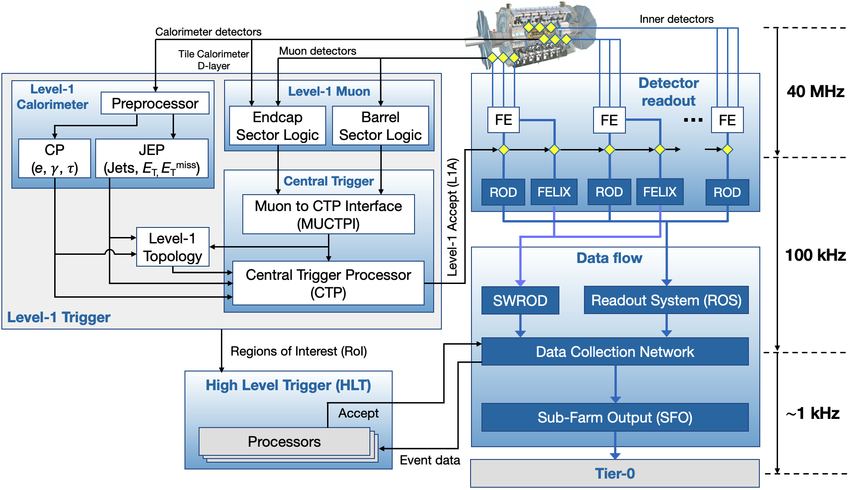
\includegraphics[width=0.8\textwidth]{figures/atlas/atlas_trigger_system.png}
\caption{A schematic showing the data flow in the trigger chain. Data is read out to both the L1Calo and L1Muon systems where logic is performed. These outputs from these triggering systems are then passed onto the CTP to determine if this event is worth a more in-depth analysis. Finally, the event information is passed onto the High Level Trigger where the final decision of whether the event is recorded or not is decided. Taken from~\cite{atlas_trigger_system}.}\label{fig:atlas_trigger_chain}
\end{figure}

\subsubsection{High Level Trigger}\label{sec:atlas_hlt}
The High Level Trigger (HLT) is the second stage of the ATLAS trigger system. It is a software based, asynchronous distributed computing system designed to reduce event rates from the 75 kHz output of the L1 trigger to about 200 Hz. The HLT is split into the two components: the Level-2 (L2) trigger which reduces event rates to about 2 kHz and the Event Filter (EF) which further reduces event rates to the final target of 200 Hz. Unlike the L1 trigger, both L2 and EF have access to the full granularity of the data collected from the detector. While these triggers are afforded more time for decision making, they still must make decisions quickly enough to maintain the output rate from the L1 trigger. The L2 trigger must make a decision in about 40 ms, and the EF in under 4 seconds. However, CPU allocation is dynamic between L2 and EF thus these timing constraints are more flexible than strict. 

\chapter{Data and Monte Carlo Simulations}\label{ch:data_mc}

\chapter{Event Reconstruction}\label{ch:reco}

\chapter{Artificial Neural Networks}\label{ch:nn}

\chapter{The VH Analysis}\label{ch:vh_analysis}
WH and ZH analysis overview goes here

\chapter{Inclusive Measurement Results}\label{ch:vh_inclusive_results}
Discuss the VH analysis inclusive measurement results here

\chapter{Simplified Template Cross Section Measurement Results}\label{ch:vh_stxs_results}
Discuss the VH analysis STXS measurement results here

\chapter{Conclusion and outlook}\label{ch:conclusions}
Discuss conclusions and outlook

% Sheep are fabulous creatures.  The noises they make are truly stupendous
% \cite{Bah}.  We also want to refer to figure \ref{fig:circle} here.
% Here's some verbatim text to screw us up:

% {\small
% \begin{verbatim}
% xxx := y;
% xy := x;
% \end{verbatim}
% }

% \begin{figure}
%   \begin{center}
%     \begin{picture}(300,200)
%       \put(150,100){\circle{150}}
%       \put(1,1){\framebox(298,198){}}
%     \end{picture}
%     \caption{A circle in a square.}\label{fig:circle}
%   \end{center}
% \end{figure}

% \subsection{All about sheep noises}
% Lots of text here just to fill up some space so we can be sure that we
% really are double-spacing and doing all the other things that might be
% necessary in formatting a dissertation to U.Mass. guidelines.  We're
% also going to have another figure here, figure \ref{fig:disc}, just
% for fun, and to make sure that the list of figures is formatted
% correctly.  Now it's time for table \ref{table:somenumbers}.  We
% really are going to need a third figure, figure \ref{fig:discs}, two
% more tables, table \ref{table:morenumbers} and table
% \ref{table:evenmorenumbers} and a fourth figure, figure
% \ref{fig:circleanddisc}, just to really make sure.

% \begin{figure}
%   \begin{center}
%     \begin{picture}(300,200)
%       \put(150,100){\circle*{150}}
%       \put(1,1){\framebox(298,198){}}
%     \end{picture}
%     \caption{A disc in a square.}\label{fig:disc}
%   \end{center}
% \end{figure}

% \begin{table}[htbp]
%   \begin{center}
%     \caption{Some numbers.}
%     \label{table:somenumbers}
%     \begin{tabular}{|r|lll|}
%       \hline
%       & Minimum & Average & Maximum \\
%       Type of Animal & Observed & Observed & Observed \\ \hline
%       Cats & 12 & 20 & 24 \\
%       Dogs & 20 & 20 & 20 \\ \hline
%     \end{tabular}
%   \end{center}
% \end{table}

% \begin{figure}
%   \begin{center}
%     \begin{picture}(400,200)
%       \put(100,100){\circle*{150}}
%       \put(300,100){\circle*{150}}
%       \put(1,1){\framebox(398,198){}}
%     \end{picture}
%     \caption{Two discs in a rectangle.}\label{fig:discs}
%   \end{center}
% \end{figure}

% \begin{table}[htbp]
%   \begin{center}
%     \caption{More numbers.}
%     \label{table:morenumbers}
%     \begin{tabular}{|r|lll|}
%       \hline
%       Type of Animal & Arms & Legs & Ears \\ \hline
%       Person & 2 & 2 & 2 \\
%       Dog & 0 & 4 & 2 \\ \hline
%     \end{tabular}
%   \end{center}
% \end{table}

% \begin{table}[htbp]
%   \begin{center}
%     \caption[Even more numbers; together with a caption long enough to ensure that multi-line caption formatting works correctly.]{Even more numbers; together with a caption long enough to ensure that multi-line caption formatting works correctly.  If you want a shorter caption to appear in the Table of Figures you're going to have to put the shorter caption in the \texttt{[]} as shown in this example.}
%     \label{table:evenmorenumbers}

%     \begin{tabular}{|r|lll|}
%       \hline
%       x & 1 & 1 & 1 \\ \hline
%       y & 2 & 2 & 2 \\
%       z & 3 & 3 & 3 \\ \hline
%     \end{tabular}
%   \end{center}
% \end{table}

% \begin{figure}
%   \begin{center}
%     \begin{picture}(400,200)
%       \put(100,100){\circle{150}}
%       \put(300,100){\circle*{150}}
%       \put(1,1){\framebox(398,198){}}
%     \end{picture}
%     \caption{A circle and a disc in a square.  We want this caption to
%       be very long to ensure that the formatting of very long captions
%       is handled correctly.  The case of short captions has already
%       been dealt with.}\label{fig:circleanddisc}
%   \end{center}
% \end{figure}



% \subsubsection{Baahs}
% \subsection{Even more about sheep noises}
% \subsection{And yet more about sheep noises}

% \section{What about wolves?}
% What about wolves?\footnote{To be fair, some wolves are probably nice\ldots}

% \section{What about shepherds?}
% What about shepherds?  I don't really know, but I want some text here
% to fill things in so that I can verify that everything is OK.%
% \footnote{Some shepherds are good, some are bad. The reader is referred
%   to Mary and The Boy Who Cried Wolf for further insight into this
%   much-debated issue. (This needs to be a very long footnote so we can
%   test the spacing between lines on a footnote.)}
% \subsection{A subsection}
% This is a subsection of the subsection about shepherds.
% \subsection{Another subsection}
% This is another subsection of that section.
% \subsubsection{A subsubsection}
% This is a subsubsection of that subsection that will in turn havae a
% paragraph with a pair of subparagraphs.  I am aware that I shouldn't
% have only one subsubsection in the subsection...
% \paragraph{A Paragraph} 
% This is the text associated with this paragraph.  I really want enough
% text to make it look like a paragraph.  Baah, baah, baah.  Baah, baah,
% baah.  Baah, baah, baah.  Baah, baah, baah.  Baah, baah, baah.  Baah,
% baah, baah.  Baah, baah, baah.  Baah, baah, baah.  Baah, baah, baah. 
% \subparagraph{A Subparagraph} 
% This is the text associated with this subparagraph.  Baah, baah, baah.
% Baah, baah, baah.  Baah, baah, baah.  Baah, baah, baah.  Baah, baah,
% baah.  Baah, baah, baah.  Baah, baah, baah.  Baah, baah, baah. 
% \subparagraph{Another Subparagraph}
% Better not have subparagraphs without text in them.  Baah, baah, baah.
% Baah, baah, baah.  Baah, baah, baah.  Baah, baah, baah.  Baah, baah,
% baah.  Baah, baah, baah.  Baah, baah, baah. 
% \paragraph{Another Paragraph}
% Baah, baah, baah.  Baah, baah, baah.  Baah, baah, baah.  Baah, baah,
% baah.  Baah, baah, baah.  Baah, baah, baah.  Baah, baah, baah.  Baah,
% baah, baah.  Baah, baah, baah.  Baah, baah, baah.  Baah, baah, baah.
% Baah, baah, baah.  Baah, baah, baah.  Baah, baah, baah.  Baah, baah,
% baah.  Baah, baah, baah.  Baah, baah, baah.  Baah, baah, baah.  Baah,
% baah, baah.  Baah, baah, baah.  Baah, baah, baah.

% Baah, baah, baah.  Baah, baah, baah.  Baah, baah, baah.  Baah, baah,
% baah.  Baah, baah, baah.  Baah, baah, baah.  Baah, baah, baah.  Baah,
% baah, baah.  Baah, baah, baah.  Baah, baah, baah.  Baah, baah, baah.
% Baah, baah, baah.  Baah, baah, baah.  Baah, baah, baah.  Baah, baah,
% baah.  Baah, baah, baah.  Baah, baah, baah.  Baah, baah, baah.  Baah,
% baah, baah.  Baah, baah, baah.  Baah, baah, baah.
% \subsubsection{Another Subsubsection}
% With some text.  Baah, baah, baah.  Baah, baah, baah.  Baah, baah,
% baah.  Baah, baah, baah.  Baah, baah, baah.  Baah, baah, baah.  Baah,
% baah, baah.  Baah, baah, baah.  Baah, baah, baah.  Baah, baah, baah. 

% \chapter{Sheep and Grass}

% \section{Introduction}

% Grass is a wonderful food...  Baah, baah, baah.  Baah, baah, baah.
% Baah, baah, baah.  Baah, baah, baah.  Baah, baah, baah.  Baah, baah,
% baah.  Baah, baah, baah.  Baah, baah, baah.  Baah, baah, baah.  Baah,
% baah, baah.  Baah, baah, baah.  Baah, baah, baah.  Baah, baah, baah.
% Baah, baah, baah.  Baah, baah, baah.  Baah, baah, baah.  Baah, baah,
% baah.  Baah, baah, baah.  Baah, baah, baah.  Baah, baah, baah.  Baah,
% baah, baah.  Baah, baah, baah.  Baah, baah, baah.  Baah, baah, baah.
% Baah, baah, baah.  Baah, baah, baah.  Baah, baah, baah. 

% \chapter{A Wonderfully Long Chapter Title That Is This Long In Order
%   to Test the Chapter Heading Stuff}
% Note that we shouldn't really have a chapter heading with no body, so
% here is a body for this chapter.  Baah, baah, baah.  Baah, baah, baah.
% Baah, baah, baah.  Baah, baah, baah.  Baah, baah, baah.  Baah, baah,
% baah.  Baah, baah, baah.  Baah, baah, baah.  Baah, baah, baah.  Baah,
% baah, baah.  Baah, baah, baah.  Baah, baah, baah.  Baah, baah, baah.
% Baah, baah, baah.  Baah, baah, baah.  Baah, baah, baah.  Baah, baah,
% baah.  Baah, baah, baah.  Baah, baah, baah.  Baah, baah, baah.  Baah,
% baah, baah.  Baah, baah, baah. 

% \section{The antidisestablishmentarainism supercalifragilisticexpialidocious longlonglonglonglongword}

% A \texttt{quotation}:

% \begin{quotation}
% Lorem ipsum dolor sit amet, consectetur adipiscing elit. Ut nibh orci, molestie
% non vehicula ac, ultricies quis purus. Nunc euismod metus vel nulla sodales quis
% tempus nisi varius. Sed ornare pulvinar bibendum. Ut egestas mollis nisi vel
% cursus.
% \end{quotation}

% \dots and a \texttt{quote}:

% \begin{quote}
% Ut dolor libero, blandit tristique accumsan non, viverra a magna. Sed pretium
% sollicitudin neque, sit amet ornare lorem convallis ac. Fusce mollis gravida
% aliquam. Nullam vulputate turpis vitae orci porttitor auctor. Donec in auctor
% erat.
% \end{quote}



%% End of body
%%%%%%%%%%%%%%%%%%%%%%%%%%%%%%%%%%%%%%%%%%%%%%%%%%%%%%%%%%%%%%%%%%%%%%%%%%%%%%%

\appendix
\chapter{THE FIRST APPENDIX TITLE}
...
\chapter{THE SECOND APPENDIX TITLE}
...

%%
%% Beginning of back matter
\backmatter{}  %% <--- mandatory

%%
%% We don't support endnotes

%%
%% A bibliography is required.
\interlinepenalty=10000  % prevent split bibliography entries
% \bibliographystyle{umassthesis}
%otherwise citations not in order for some reason
\bibliographystyle{unsrturl}
\bibliography{thesis}
\end{document}

%%% Local Variables: 
%%% mode: latex
%%% TeX-master: t
%%% End: 
